%% REVISE FOR KEYWORD-ABBREVIATION REFERENCES and ABBREVIATION DETAILS
%%% CHAPTER Introduction ------------------------------begin----
%Quotes to have

\chapter{Introduction} \label{introductionchapter}
\section{Motivation}
Developing and distributing effective software is one of the most important concerns of today's software-driven fields. Effective software is surely needed in almost every part of embedded systems, especially in the fields of automotive, robotics, defense, transportation, electrical instruments, autonomous and cyber-physical systems. Quality software involvement in fields such as the ones that are mentioned created a great demand for parallel software development in the last ten years. This great demand caused software engineers in especially IT and embedded system sector to study parallel computing along with multi- and many- core systems.

The digitalization of almost every aspect of our lives as we know it requires systems to be more and more complex each passing day. While some years ago the computers had single-core processors, today almost every single computer has at least a couple of cores in their processors. The advancements in processors allowed development of more advanced systems with efficient software. The super computers currently NASA (The National Aeronautics and Space Administration) uses for collecting information are said to record as much data as it has been collected in the entire the world history in just four years. This example should show that how complex applications can be in the century we are living in. Furthermore, one of the most trending topics Cloud Computing, which is being studied to make use of complex computing power of super computers' remotely to public users, is being researched and it will benefit greatly from the advancements in the field of parallel computing.

While parallel computing is used for achieving more complex software, it is also widely used in more basic and cheap processors in order to achieve more tasks with less resource consumption and cost. This is achieved by proper scheduling techniques. Furthermore, with an efficient software distributed efficiently to a processor's cores, one could also make use of less energy consumption features by applying techniques such as under-clocking a processor. To summarize, developing efficient parallel software is not only useful in achieving advanced computing capability but also can help to achieve less energy and resource consumption, thus decreasing the cost of systems and making them more environment-friendly.

\section{Objective}
Even though achieving concurrency using parallel computing is crucial, it might lead to error-prone systems if software is not planned and executed properly. Developers have to consider using the right software and also have to determine and plan not only the hardware constraints but also the software constraints in order to create an efficient and reliable software.

Before its execution, parallel software have to be delicately planned. The first stage of the parallel software development, planning stage, involves several activities such as Modeling, Partitioning, Task generation and Mapping. In the modeling stage, hardware and software model needs to be created. While software model is described by defining runnables, labels, label accesses, runnable activations and software constraints; the hardware model is described by defining processor details, hardware system clock and core information. After the modeling activity, partitioning is done that determines which group of runnables belong together. Partitioning results are combined with system constraints in order to generate tasks. Final activity, Mapping, involves laying out the details about pinning generated tasks to available hardware units and their cores.

While there are some commercial tools that provide easement in the parallel software development, recent study done in Germany, namely AMALTHEA4public \cite{ICPDSSE} \cite{amalthea4publicweb}, aims to provide planning and tracing tools especially for multi-core developments in automotive domain with several open source development tools. The branch of AMALTHEA4public, APP4MC project \cite{app4mcproposaleclipse} provides an Eclipse-based tool chain environment and de-facto standard to integrate tools for all major design steps in the multi- and many-core development phase. A basic set of tools are available to demonstrate all the steps needed in the development process. The APP4MC project aims at providing \cite{app4mcproposaleclipse}:

\begin{itemize}
	\item A basis for the integration of various tools into a consistent and comprehensive tool chain.
	\item Extensive models for timing behaviour, software, hardware, and constraints descriptions (used for simulation / analysis and for exchange).
	\item Editors and domain specific languages for the models.
	\item Tools for scheduling, partitioning, and optimizing of multi- and many-core architectures \cite{app4mcproposaleclipse}.
\end{itemize}

The author aims to investigate and evaluate APP4MC's performance with real-world distributed multi-core system in several aspects. The objectives of this project could be listed as follows:
\begin{itemize}
	\item Development of a distributed multi-core demonstrator for the APP4MC platform that involves features with the emphasis of automotive applications.
	\item Investigation of new trends in parallel software development (such as Real-time Linux parallel programming, POSIX threads, RTOS, evaluation methods etc.)
	\item Researching techniques to retrieve information (number of instructions, communication costs) and system trace from platforms such as xCORE and Linux to achieve precise modelling with APP4MC.
	\item In order to achieve optimization goals such as reduced energy consumption and reduced resource usage, different affinity constrained software distributions will be evaluated and energy features will be invoked to see if the goals are met.
	\item Developing a basic online parallelization evaluation software that will retrieve scheduling properties such as slack times, execution times, and deadlines from all the processes and that will tell how many of the deadlines are met, how good of a software distribution it is while the software is being executed. Also, investigating methods to develop threads and processes that are schedulable.
	\item Also taking system traces from the software to carry out offline software evaluation in order to figure out means to balance the load on cores.
	\item Comparing the conventional schedulers non-constrained affinity distribution (such as a Linux OS scheduler) to the affinity constrained distribution from APP4MC to see if performance can be improved.
\end{itemize}

With the help of A4MCAR project it is intended that the Real-time Linux community will benefit from the published libraries and documentation that involve code snippets and information instructions on how to develop more optimized distributed and parallel software. Furthermore, the Eclipse and APP4MC community will benefit from the A4MCAR via advanced tool support for RPI developments, open source example applications, and validations of APP4MC parallelization results in order to create a better tooling for public. Those results can be used to assess and compare different parallelization scenarios and consequently identify optimal solutions regarding timing efficiency for the A4MCAR. Thereby, a point of reference can be given as well as an easy starting point for developers approaching parallelism with their developments. 

\section{Methodology}

Automotive or any vehicle control related field tends to require very complex systems. In a real-life automotive application, amount of hardware nodes and software nodes are high in number. Since the main focus of the APP4MC environment is to provide parallel computation tools for automotive domain, a demonstrator is required that is closely related to automotive domain and that can be used for troubleshooting APP4MC. For that purpose, a demonstrator RC-Car called A4MCAR is developed. Although an RC-Car does not match up the number of nodes used in real vehicles, the A4MCAR has several nodes and a distributed architecture, thus matching a vehicle's distributed architecture such as the AUTOSAR used in vehicles. Furthermore, A4MCAR can be used for automotive-like applications that involve motor driving, navigation, sensor driving, and autonomous features.

The demonstrator, A4MCAR, is equipped with a distributed architecture that involves a 16-core multi-core microcontroller development board (XMOS xCore-200 eXplorerKIT) and a 4-core single board computer (Raspberry Pi 3) with Linux OS. The software nodes with respect to their priorities and low-level and high-level purposes are distributed along those hardware modules. The demonstrator is not only designed to match up the capabilities of a real vehicle but also involves parts that are related to semi-autonomous driving and control. It can handle wifi and bluetooth connection requests and drive itself accordingly over a web interface or an Android application. Since A4MCAR is specifically designed as a demonstrator, it has the capability to monitor and visualize core utilization and display it using a touchscreen or its web interface. Furthermore, it is equipped with four ultrasonic sensors and a camera with image processing embedded to support its autonomous driving and web interface streaming functions.

In this paper, the development and parallelism evaluation of the demonstrator A4MCAR as well as the studies on parallel computing and tracing options are discussed. Obtained results are used in APP4MC for better development. The remainder of this paper is organized as follows: Chapter \ref{multicorechapter} is dedicated to background information on concurrent programming and design with APP4MC while Chapter \ref{designchapter} is dedicated to explaining demonstrator design and implementation. After Chapter \ref{designchapter}, Chapter \ref{informationchapter} and Chapter \ref{evaluationchapter} will involve Information Tracing and System Management and Results, respectively. The paper will be concluded with Chapter \ref{conclusionchapter}.

%%% CHAPTER Introduction ------------------------------end----
%%% CHAPTER Multi-core Programming ------------------begin----
\chapter{Background Information on Concurrent Programming and APP4MC} \label{multicorechapter} 
\section{Introduction to Parallelism} %why parallelism, Distributed and parallel architectures, Multicore processors
High performance systems, scientific computations and multi-feature systems require well-established parallel software. The physical problems in our world are being solved by computer systems by making use of simulations which are becoming more and more complex as the years go by. Graphical applications which involve big data operations also make use of the benefits of the parallel software. As the data that is involved in such systems increase, required amount of computing power, memory space and the need for accuracy and speed also increases. In the last decades, the improvements in high performance computing and the advancements in processors are significantly developed which allows the development of efficient parallel software in systems. Today, computers with multicore processors allow every desktop to be eligible for parallel software development. In \cite{springerparallel}, it is pointed out that the technological developments regarding multi-core processors and parallel computing was forced by physical reasons. As increasing the clock speed causes overheating which gets harder and harder to get rid of as the clock speed increases, the developments regarding multi-core technology allowed more computations to be achieved without having to increase the clock frequency \cite{springerparallel}.

While the hardware-related developments are out there, in order to make use of parallelism one should modify an existing software to increase its performance on a multi-core processor. Furthermore, the execution time of the parallel program should be lesser the execution time of the sequential program for it to worth the effort. Designing a parallel program, as compared to a sequential program could be time consuming. In this regard, one should know how the parallel programming models and modern techniques to utilize a software in parallel manner. With this idea, it can be said that there is much research going on in the area of parallel programming languages and environments with the goal of utilizing parallel programs at the right level of abstraction \cite{springerparallel}.

The following sections in this chapter will give an introduction to parallelism, modern techniques, and will explain the theoretical part of parallelism which is addressed in this report.
\section{Memory Architectures} 
Parallelization of a program is all about efficient usage of CPU time (also called as computation time) and memory access. Assuming some tasks are distributed through a distributed, many-core or multi-core system, the synchronization between the tasks' access to memory should be achieved. With these goals in mind, machines according to their memory architectures could be summarized as follows:
\begin{itemize}
	\item \textbf{Distributed Memory Machines (DMM):} Distributed Memory Machines are the systems that use distributed memory architecture. A DMM is illustrated in the Figure \ref{fig:memarch}. In the distributed memory architecture, the units which consist of a processor and a memory are interconnected using a network \cite{springerparallel}. There are several topologies with which the nodes can be interconnected. Such topologies involve point-to-point topology, bus topology, crossbar topology, ring topology, mesh topology and hypercube topology which makes use of an external routing unit \cite{interconnection}. The advantage of distributed memory is that each processing unit has individual memory units. Thus, all local memory is private and can only be accessed via the respective local processor. Therefore, the communication between the individual processor memories are only handled via a \textbf{message passing interface (MPI)} \cite{springerparallel}. However, DMMs often have very large communication costs compared to other memory architectures. DMMs often resemble networks of workstations according to \cite{springerparallel}. Collection of complete computers with a dedicated interconnection network are called \textbf{clusters} and they also use message passing interfaces for communication. The difference between cluster systems and distributed systems is that a job scheduler is used in clusters as opposed to being addressed individually. Today's popular message passing libraries to address communication in cluster systems and distributed systems involve PVM and MPI libraries \cite{springerparallel}. 
	\item \textbf{Shared Memory Machines (SMM):} Shared Memory Machines are the systems that use the shared memory architecture. Since shared memory architecture has a \textbf{shared physical memory (global memory)}, the coordination of processor accesses to global memory should be considered. A global memory can be a collection of memory modules and the data access to the global memory is handled by reading or writing \textbf{shared variables}. A shared memory architecture is illustrated in the Figure \ref{fig:memarch}. A typical example of a shared memory architecture can be found in \textbf{multi-core processors} in which there exists many physical processing units called \textbf{cores}, and shared memory modules. In computers, parallel programs for SMMs are often handled by using \textbf{threads} which are control flows which shares data with other threads by accessing a global address space. While \textbf{kernel threads} are managed by \textbf{operating system (OS)} and mapped to the system cores by the OS, the \textbf{user threads} are often mapped to cores by using specific programming environments. Today's user threads within a computer system often use frameworks and libraries such as OpenMP and POSIX thread (Pthread) for C language, Java Threads, and Python's 'threading' library \cite{springerparallel}. 
	
	While using shared memory architecture is advantageous in terms of costliness, the design of shared variables and mutual exclusion of shared variables might be effortful and time consuming. The coordination problems of shared address space may lead to error-prone non-deterministic systems which will have the issues such as \textbf{race conditions} which will be described in the coming sections. 
\end{itemize}
\textbf{Distributed Shared Memory (DSM)} architecture is often used in systems as well. A depiction of such an architecture is given in the Figure \ref{fig:memarch}. In distributed shared memory, the shared memory model is implemented in distributed systems. Shared memory model allows all nodes to have virtual memory space. Since distributed systems have high communication costs, by moving data to the location of access, the DSM systems reduce the high communication cost \cite{dsm}. 
\begin{figure}[!ht]
	\centering
	\captionsetup{justification=centering}
	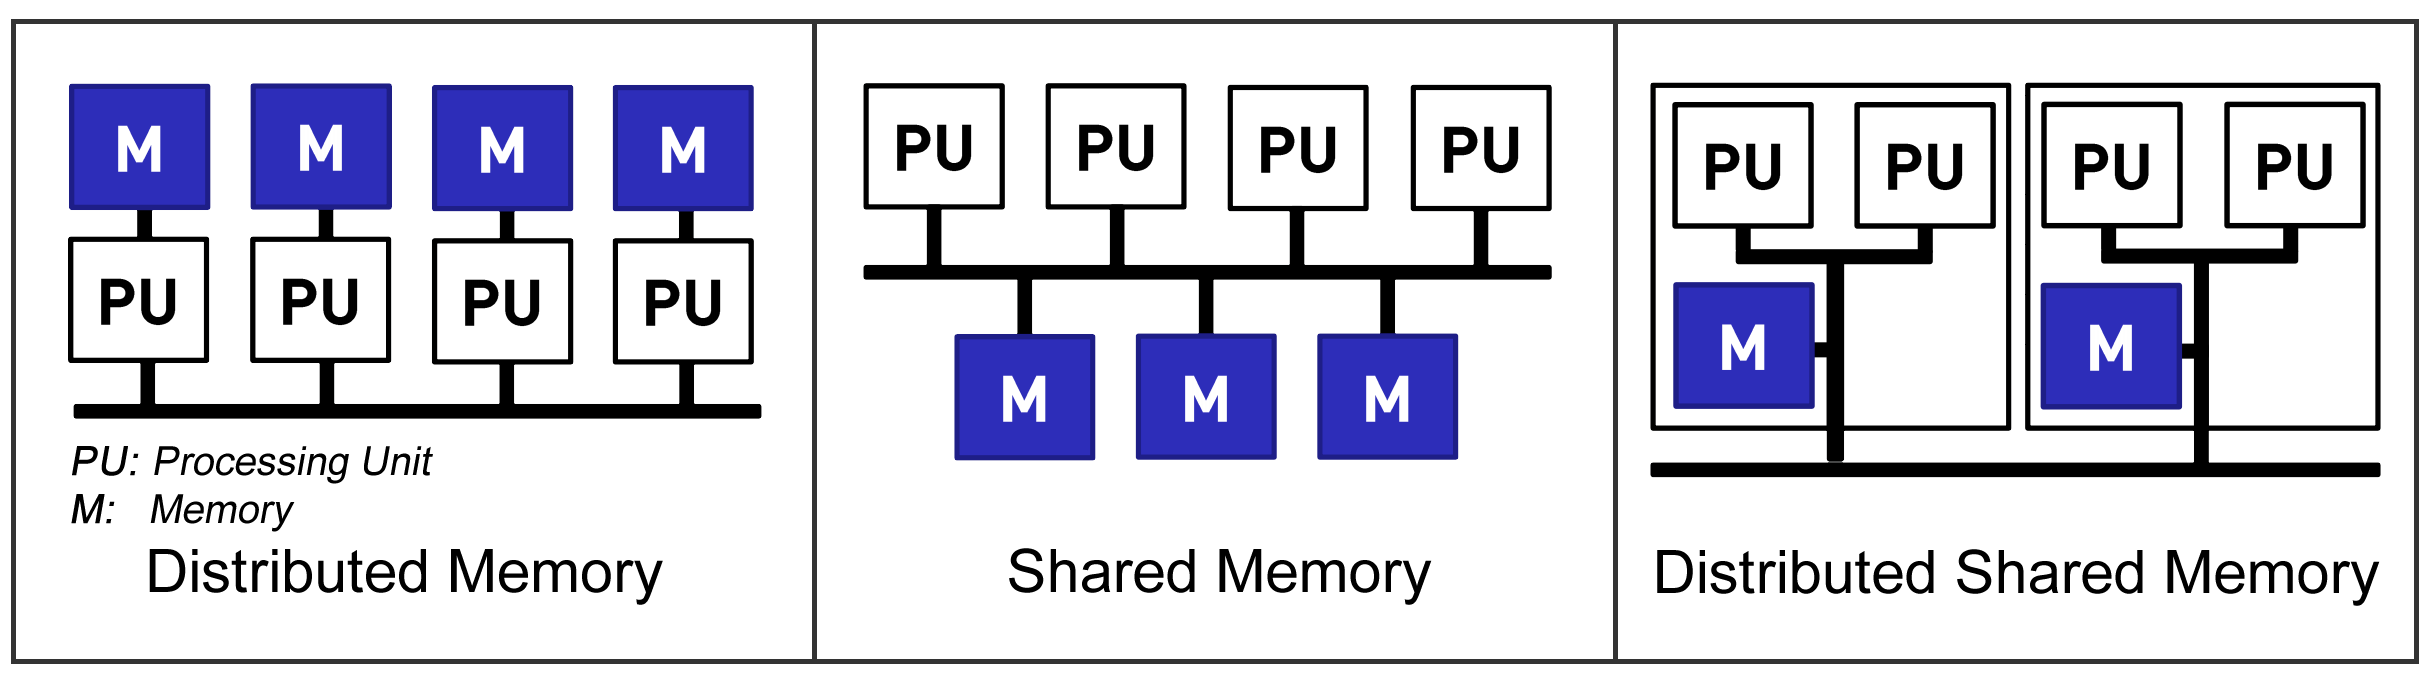
\includegraphics[width=\textwidth]{content/images/memarch.png}
	\caption{Memory Architectures \cite{lukas1}}
	\label{fig:memarch}
\end{figure}
%memory architectures

\section{Introduction to Multi-core Processors} %pp. 26
The processor chip technology is being developed progressively for many past years. However, according to \cite{springerparallel}, the fashion of increasing the chip performance has changed due to the physical limitations. As an example, pipelined parallelism of instruction execution is limited by the clock speed. The Parallel Programming book by Thomas Rauber et al. \cite{springerparallel} explains these limitations as follows:
\begin{itemize}
	\item Clock speed of a processor can no longer be increased significantly. Since the increase of the number of transistors on a chip is achieved by increasing the transistor density and this results in excessive heating due to current leakage, expensive cooling equipment are required. Furthermore, the heating on a chip should not exceed a certain limit to keep the chip functioning properly.
	\item Memory access times can not be reduced as the same rate as the processor clock increase. That results in a bottleneck when the processor is accessing the memory. \textbf{Cache memories}, which are the temporary memories that are used in order to reduce the memory access times, are used in order to overcome this issue but further performance increase in processing units may not be resolved with caches.
	\item The speed of signal transfers within the wires could be a limiting factor.
	\item The physical size of a chip limits the number of pins that are used, which can limit the bandwidth between CPU and memory, which will also create a bottleneck at the memory communication.
\end{itemize}
Due to the aforementioned limitations, rather than increasing the performance, multi-core processors have been developed which consist of several physical execution cores. Due to the physical cores, total parallelism as opposed to single-core threading is achieved by using multi-core processors. Cores of a multi-core processor consist of seperate execution resources such as functional units (Arithmetic Logic Unit (ALU), multiplier) and execution pipelines \cite{springerparallel}. A multi-core processor or a microcontroller also fits in a single chip package same as a single-core processor. Proper software application examples in a multi-core computer system involve background applications and scientific cpu-intensive computations that distribute a task into several cores to improve their performance.

Within a multi-core processor, usage of threads should also be understood. It is known that the single-core processor threading can be used to achieve parallel software with higher performance. The threading is also possible in multi-core processors which will achieve even higher performance and will allow more features to be parallelized. The graphical illustration of this is given with the Figure \ref{fig:differentthreading}. Using the physical core for only one thread or a process is related to \textbf{mapping}, whereas the timing organization of many threads in one core is handled by \textbf{scheduling} which is done by the operating system. These terms will be further explained in the coming sections.

\begin{figure}[!ht]
	\centering
	\captionsetup{justification=centering}
	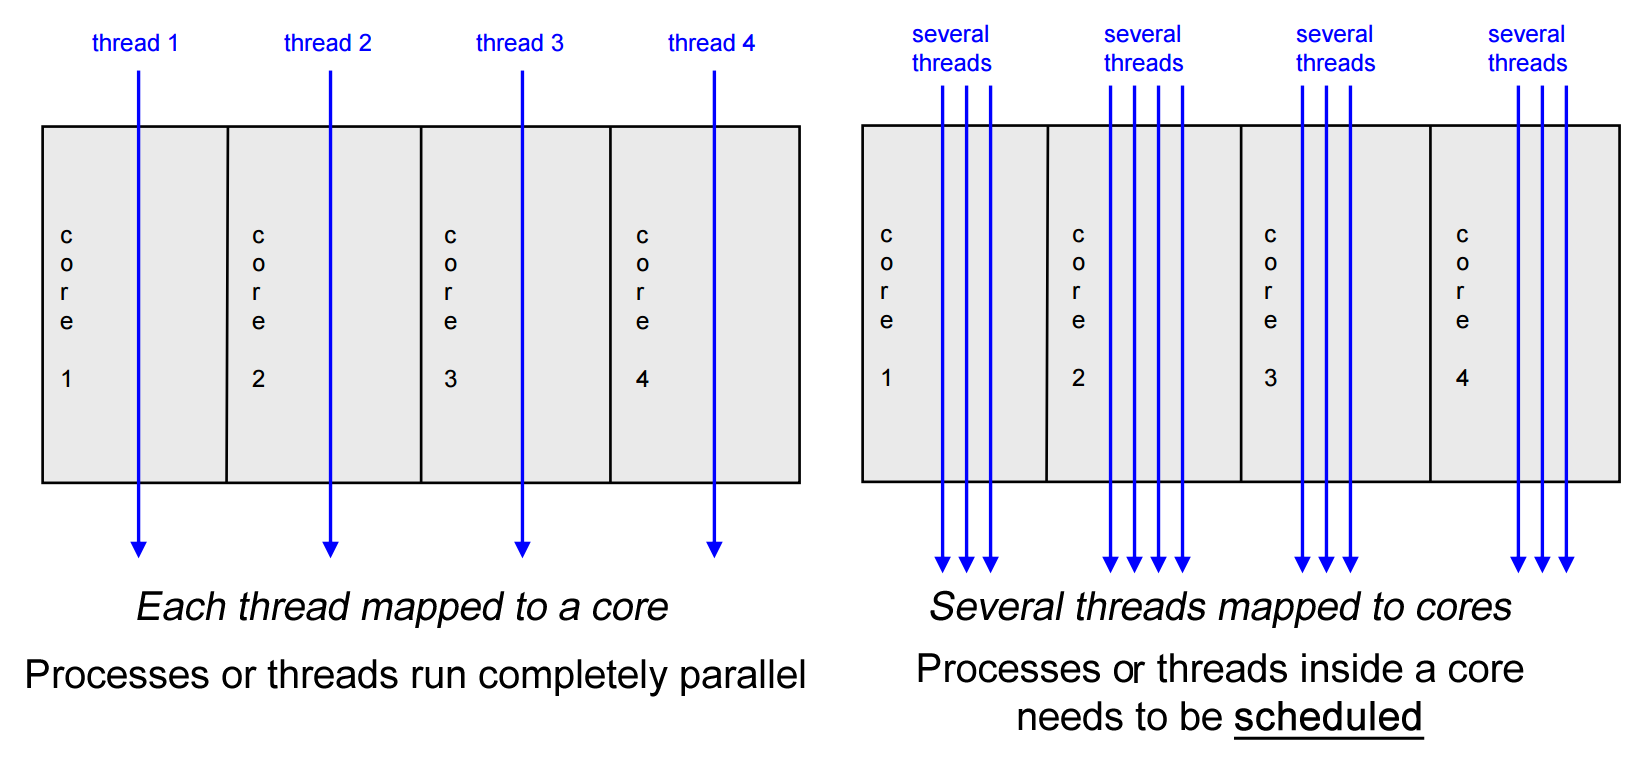
\includegraphics[width=\textwidth]{content/images/differentthreading.png}
	\caption{Illustration of time-sliced execution paths in a multi-core processor \cite{multicore1}}
	\label{fig:differentthreading}
\end{figure}

\section{Essential Concepts in Parallelization} 
%basic concepts terminology
%terminology: intro, process, task ,thread, runnable etc
%levels of parallelism

Basic concepts in parallel programming should be understood to develop efficiently utilized software. The design of a parallel software starts by decomposing an application into its smallest pieces which are called \textbf{runnables}. One or more runnables combined constitute \textbf{tasks} which are functional pieces of an application that can be executed parallel across a multi-core or single-core processor. The size of tasks (mostly in terms of number of instructions) are called \textbf{granularity} \cite{springerparallel}. Therefore, when decomposing an application into smaller pieces, granularity of the tasks should be considered for the load balancing. The tasks of an application are assigned to processes or threads for parallel execution on the hardware platform. Therefore, \textbf{process} can be defined as a program in execution that is assigned to execution resources for execution. The switching between processes are called \textbf{context switches}, and the \textbf{scheduler} of the operating system manages those switches. A \textbf{thread} can be defined a continuous sequence of execution. A process can involve one or many independent control flows, i.e. threads \cite{springerparallel}. 

\textbf{Scheduling} is the process of determining the order of execution of processes or threads on physical hardware whereas \textbf{mapping} is defined as the assignment of processes or threads on processing units. In other words, processes or threads are placed on cores using mapping, whereas their execution sequence is determined programmatically with the help of scheduling. Usage of these techniques for parallel design brings their own challenges Besides assigning processes or threads to cores, one should also manage assigning data to memories and communication to data paths. Constraints such as instruction set, locality /grouping,  sizes, and deadline of the tasks can make this process effortly and time consuming \cite{lukas1}. \textbf{Synchronization} is also an important job which defines the organized communication between processes or threads \cite{springerparallel}. Since the memory organization of the hardware matters, design should consider the hardware along with the software. The coordination and synchronization of processes and threads will be discussed in the next section.

Finding a useful scheduling and mapping strategy is key to parallel design. The practices involve keeping the \textbf{parallel execution time} of a task lower than the \textbf{sequential execution time}, keeping the load balanced through the cores of the system and keeping the communication overhead low. According to the book \cite{springerparallel}, for the quantitative evaluation of parallel programs, measures such as \textbf{speedup} and \textbf{efficiency} can be used which are the measures that compare parallel execution time of a software with its sequential execution time.

\section{Design Techniques in Parallelization} \label{designtech}
%co-design stages etc. % involves co-design stages (parallelization of programs pp.108) partitioning mapping egc. + Also advantages and disadvantages 
Parallelization can be defined as the transformation of a sequential program into a parallel program \cite{springerparallel}. Although different sources (\cite{springerparallel} and \cite{lukas1}) generalize the design techniques in parallelization differently, one can go through the following challenges in order to develop parallel software through parallelization (also illustrated with the Figure \ref{fig:designtechniques}):
\begin{figure}[!ht]
	\centering
	\captionsetup{justification=centering}
	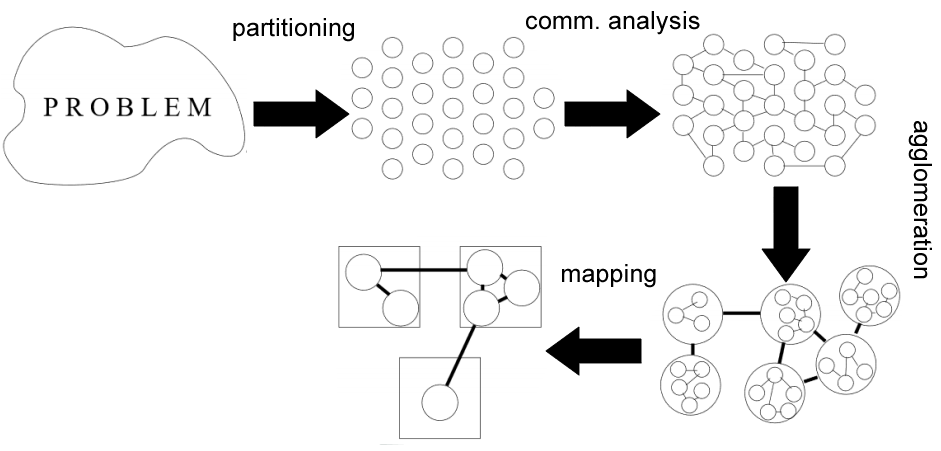
\includegraphics[width=\textwidth]{content/images/designtechniques.png}
	\caption{Illustration of design techniques in parallelization \cite{lukas1}}
	\label{fig:designtechniques}
\end{figure}

\begin{itemize}
	\item \textbf{Partitioning of the problem:}
	The application that addresses a problem should be decomposed into smaller pieces, i.e. runnables that are considered to be smallest pieces in a software. In some cases, this decomposition can be at task-level. A runnable or a small task can be a function that involves a single read or write access to a register or a shared variable, peripheral communication, or simple computations. In theory, a runnable is only executed in a single core and it has no dependencies to another runnables. The goal of this decomposition (according to \cite{springerparallel}) is to make sure that all the applications are fine-grained enough that the load balancing can be achieved. In other words, runnables have small granularity and with the help of this the generated tasks can be distributed more efficiently.
	\item \textbf{Analysis of the communication:} Communication between runnables and tasks should be considered before the task generation. Communication is a big constraint in a parallel software, therefore all the dependencies between runnables or tasks, in terms of which runnable reads or writes data, and what is the communication cost (granularity) should be analyzed.
	\item \textbf{Agglomeration of executables to tasks (Task Generation):}
	In the task generation phase, runnables and some tasks are grouped together in order to constitute tasks. This is done with the consideration of dependent runnables in terms of communication. Also, the grouping should consider functional unification as well it should consider load balancing. 
	\item \textbf{Assignment of tasks to processes or threads:}
	According to \cite{springerparallel}, this intermediate phase is involved in computer systems where processes and threads are involved. The tasks that are generated can be grouped in order to constitute processes or threads. This step is the step which makes the software mapping-ready. In the cases of some multi-core microcontrollers, the mapping is done at the task-level, therefore this intermediate step is not required.
	\item \textbf{Mapping of processes or threads to physical processes or cores:}
	Each process, thread, or task in some cases are assigned to a seperate processor or core after the final agglomeration phase, i.e. when the runnables are grouped sensibly. In cases where there is more process or thread than a core, multiple threads are assigned to some cores. In this case, as mentioned scheduler of the operating system takes care of the execution order of multiple processes or threads on a core. Mapping phase in computer systems is usually done by the operating system but the users can intervene. The main goal of mapping step is to get an equal utilization while keeping the communication overhead smallest \cite{springerparallel} \cite{lukas1}.
\end{itemize}

\section{Coordination and Mutual Exclusion} %mutex semaphore etc.% race cond, deadlock, livelocketc. %shared variables shf 133-134
When developing parallel programs, not managing the critical sections correctly might lead to error-prone systems. A \textbf{critical section} can be defined as a shared variable that is accessed by two or more processes or threads. The actions of the processes or threads, when accessing a critical section, should be co-ordinated. For that purpose, \textbf{mutual exclusion} (also called \textbf{mutex}) concept is studied which refers to the requirement of ensuring that no two concurrent processes are in their critical section at the same time \cite{lukas1}. Generally, the mutual exclusion is handled by using mutex algorithms such as Lamport's Bakery Algorithm \cite{lukas1}, ensuring that every process is live, safe (no non-deterministic behavior is involved) and fair amount of CPU time is granted to each process.

There are many problems that can occur in case the coordination of the process communication via accessing critical sections is not handled properly. A problem that is called \textbf{race condition} can occur in case mutual exclusion is not properly provided. Race condition can be defined as the behavior of a system where the system behavior depends on the order or timing of the uncontrollable (sporadic) events \cite{lukas1}. In other words, race condition happens when the system behaves non-deterministically due to the non-fixed order of accesses to critical region. Another problem that might arise is the \textbf{deadlock} problem which is the issue of processes not releasing the shared variables and waiting to acquire other shared variables that are being used by other processes \cite{lukas1}. In a deadlock scenerio, neither process can continue working therefore the execution does not progress. In a \textbf{livelock} situation, however, two or more processes access a shared variable but does inverting actions, thus even though the processes are alive the execution does not progress and has a non-deterministic behavior. The \textbf{spinlock}, a situation in which a task is continuously waiting for a shared variable to be released, can be given as another example of the problems that might occur if the mutual exclusion is not properly implemented.

Today, many thread and concurrent programming libraries involve functions to use mutual exclusion. A simple way to access a shared variable in a programming language could be to define a mutex variable and lock it before writing to this critical section. After the process writes to the critical section, one must release the section by unlocking the mutex variable. However, it must be remembered that while handling complex critical sections where many processes are involved, coordination of process access' to the critical section should be provided by using mutual exclusion algorithms such as Lamport's Bakery Algorithm. \textbf{Semaphores}  (which are data types that control the access of multiple processes to a shared resource), \textbf{monitors} (which provides buffered locking mechanism to concurrent accesses), and synchronization methods (such as message passing) can also be used in order to coordinate the actions of multiple processes to critical sections \cite{lukas1}\cite{springerparallel}.

\section{Analysis of Scheduling}\label{schedulingsection}%and schedulers
For the purpose of analysis and evaluation, one can use system traces that involve information such as timing, mapping, and priority in order to see if the tasks, processes or threads are scheduled properly. To meet the optimization goals, this work involves evaluation of several software distributions. 

According to \cite{lukas1}, Quality of Service (QoS) of scheduling could involve the following goals:
\begin{itemize}
	\item Even load-balancing
	\item Efficient resource usage 
	\item Maximizing throughput (completed processes per time unit) and utilization (percentage a processor is used)
	\item Minimizing response time and latency
	\item Maximizing fairness (every process receive fair amount of cpu time depending on their granularity)
	\item Avoiding starvation (every process is guaranteed to receive cpu time eventually)
\end{itemize}
In the later sections, the optimization goals for parallel software will be discussed. It can be argued that an important portion of the optimization goals for a parallel software can be achieved through the scheduling goals.

To understand how tasks are scheduled, one must carefully study the task graph given in the Figure \ref{fig:scheduling}. In the figure, it is seen that two tasks are given with Task B having a higher priority but lesser execution time. Timing properties of the given timeline could be defined as follows \cite{timingposter} \cite{lukas1}:
\begin{figure}[!ht]
	\centering
	\captionsetup{justification=centering}
	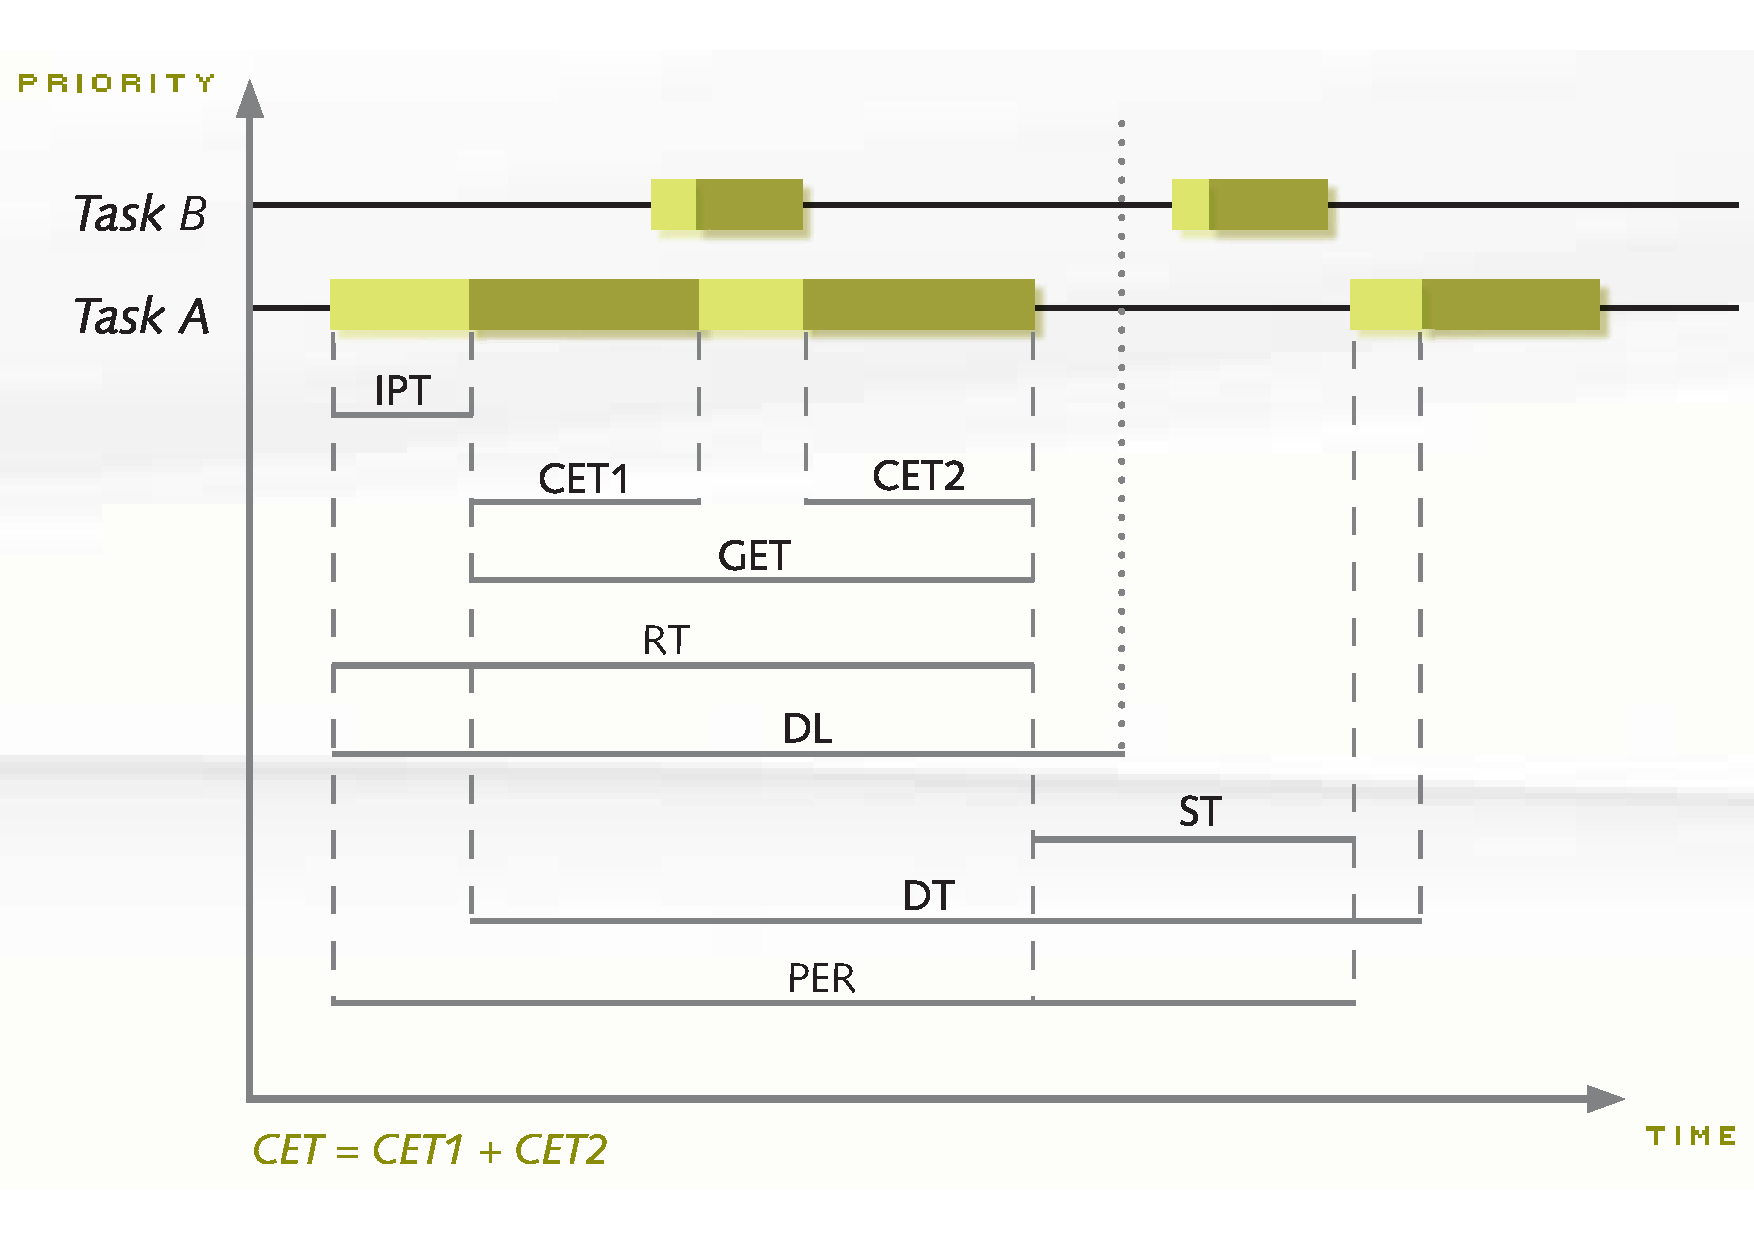
\includegraphics[width=\textwidth]{content/images/scheduling.pdf}
	\caption{Timing properties for scheduling in multi-tasked systems \cite{timingposter}}
	\label{fig:scheduling}
\end{figure}
\begin{itemize}
	\item \textbf{Initial Pending Time (IPT)}: IPT is defined as the preparation time before a task is ready to be started execution.
	\item \textbf{Core Execution Time (CET)}: CET is the absolute time elapsed at which the task is executed on the processor. Therefore, the amount of time the task is preempted are not counted when calculating the CET. In the figure, it is seen that Task A is preempted once, thus the overall CET is found by adding the times CET1 and CET2.
	\item \textbf{Gross Execution Time (GET)}: GET is the amount of time it passes for an iteration of a task or an event is executed. In other words, it is the elapsed time the execution is done until the task goes into the sleeping state.
	\item \textbf{Response Time (RT)}: Response time is calculated by adding IPT and GET. 
	\item \textbf{Deadline (DL)}: Deadline of a task or an event is the amount of time a task should be completed in order to meet the real-time requirements of the task. Therefore, a reliable task should not miss its deadline even in the worst case. The deadline misses (DLM) can be used as an evaluation measure for the reliability of a task. It can also be used as a measure to compare the quality of software distributions.
	\item \textbf{Delta Time (DT)}: Dela time of a task can be defined as the time between two gross executions of a task.
	\item \textbf{Slack Time (ST)}: Slack time is the amount of time a task is at a sleeping state. In other words, slack time is the time between the last response of a task and the start of the pending state. Slack time describes the flexibility of a task, thus it is the time that CPU can be used for other tasks. Therefore, if the slack time is higher in a task, that task is considered to be less stressed. Slack time is also a measure that is used in the evaluation of different software distributions. 
	\item \textbf{Period (PER)}: Period is one of the most basic properties of a task which defines how long it takes before a task repeats its instructions. The period is defined for tasks that are periodic.
\end{itemize}

Although the given timeline depicts the overall timing properties of task scheduling, due to tracing and instrumentation limitations not all of the information is extractable from the system trace. IPT, for example is a timing property which is not present in the tracer that is used in the work that this report explains. Therefore, IPT is neglected due to the aforementioned limitations and the fact that it is bound to be a rather small amount of time. Analysis of scheduling is implemented in this work and one should see the details in the Section \ref{onlinetiming}. Furthermore, how information of what kind of evaluation metrics are used are further explained in the Section \ref{opt}.

\section{Optimization and Evaluation of Parallel Software} \label{opt}
Not every parallel program are beneficial. In order for a parallel program to be useful, it should be optimized. There are four main reasons a parallel software should be optimized. Each optimization process focus on a goal and the design and development of the software should be carried out by considering that goal. The optimization goals (depicted in the Figure \ref{fig:optimization2})  may involve achieving lowest energy consumption, achieving lowest computation time, achieving highest resource utilization, and achieving highest reliability. The way these goals are achieved are also shown in the Figure \ref{fig:optimization2}. It should be added that maximizing or minimizing any software property in a positive way can be generally seen as an optimization problem that deals with e.g. safety, security, distributivity, or scalability demands among others. However, the figure given shows the basic software optimization goals that are related to this work.

\begin{figure}[!ht]
	\centering
	\captionsetup{justification=centering}
	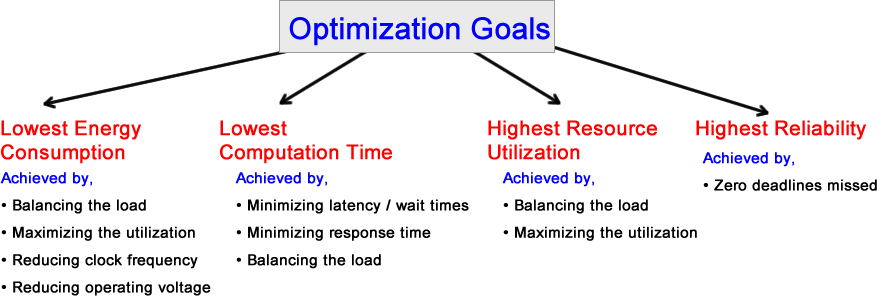
\includegraphics[width=\textwidth]{content/images/optimization2.png}
	\caption{Optimization goals of parallel software \cite{lukas1}}
	\label{fig:optimization2}
\end{figure}

On a higher level, there is always a question whether the optimized software is really optimal or not. There are strategies with which this could be measured and true optimization could be achieved \cite{lukas1}. Those strategies involve Linear Programming, Integer Linear Programming, Mixed Integer Linear Programming, Quadratic Programming, Evolutionary Algorithm, and Simulated Annealing \cite{lukas1}. Although it is useful to know such strategies exist, the optimization of an parallel software on a higher abstraction layer will not be a part of this work. 

As mentioned before, one of the most basic evaluation techniques to determine if a parallelized software is beneficial as opposed to a sequential software is to check the run-times of the processes. If the parallel run-time (overall execution time) of a program is less than the sequential run-time, then it could be said that parallelization helped in terms of computation time. The following list involved the parallelization evaluation techniques that will be a part of this work in evaluating software distributions.
\begin{itemize}
	\item ${ST\textsubscript{avg}}$: Average slack time of all traceable processes
	\item ${DLM}$: Percentage of deadlines missed
	\item ${U\textsubscript{0-p}}$: Percentage of utilization of each core
	\item ${S\textsubscript{p}(n)}$: \textbf{Speedup} value which quantitatively compares the execution time of a sequential implementation with that of the parallel implementation \cite{springerparallel}. Speedup is calculated as follows \cite{springerparallel}, given that ${T\textsuperscript{*}(n)}$ is the sequential run-time and ${T\textsubscript{p}(n)}$ is the parallel run-time:
	\begin{equation}\label{speedupeqn}
	S\textsubscript{p}(n)=\frac{T\textsuperscript{*}(n)}{T\textsubscript{p}(n)}
	\end{equation}
	It can be said that bigger the speedup value, better the parallel utilization.
\end{itemize}
The aforementioned evaluation techniques mostly can be used to evaluate load balancing (${U\textsubscript{0-p}}$), reliability (${DLM}$) and resource utilization (${ST\textsubscript{avg}}$, ${U\textsubscript{0-p}}$ and ${S\textsubscript{p}(n)}$). 
%optimization info
%parallel time < sequential time  %speedup
%metrics slack time etc..
%load balancing


\section{New Trends in Parallelization} %Real-time Parallelization Trends in Practice: RTOS, MPI, OpenMP, Pthreads, Java Threads and AUTOSAR... 
%embedded computing > single board computers >Raspberry Pi ve neden real-time olamaz..
New practical trends evolve in software development every passing day. Since today's applications are more complex than it was before, software development field is bound to grow. Surely, with the applications getting more complex, more advanced development environments, platforms, and frameworks are needed. Software engineers has been trying to fulfill this need especially since embedded, internet-based and cyber-physical systems became more common. Since some systems require hard real-time requirements, real-time development has became an important field of study.

One of the most common concurrent programming libraries involve \textbf{Real-time Operating Systems (RTOS)}.  Real-time operating systems are the operating systems or more practically frameworks that are developed for microcontrollers or processors. They provide real-time computing to the viable hardware in order to be used in the applications that requires deterministic and predictive task behavior \cite{rtos1}. RTOS' implement kernel components which are scheduler, thread managers, message queues, semaphores, mutexes, timers, and memory pools \cite{rtos1}. In the basic sense, an RTOS can be used to schedule applications, send and receive messages, get and release semaphores, and handle events in order to manage a parallel system \cite{rtos1}. RTOS' are common for both single-core and multi-core processors. With a single-core processor, many threads are scheduled within a single core whereas in a multi-core processor, the mapping features can also be used. As an example, FreeRTOS (also currently called as CMSIS OS) is a common RTOS library that is developed for ARM Cortex M series microcontrollers (such as STM32F407 or STM32F103C8T6). Another examples involve OSEK/VDX,  RTX, FreeOSEK etc.

As introduced, multi-processor and multi-core solutions are also common. For distributed systems, MPI C/C++ library uses compiler directives to parallelize applications. Furthermore, OpenMP is a C/C++ library that is developed for systems with shared memory architecture and it can be used for another solution to parallelize applications and manage message passing. 

Since thread-level parallelism, i.e. using virtual cores to manage many-tasked, advanced, featured systems, is very common since the multi-core processors became common, almost every programming language has their own separate libraries or frameworks to support multi-threaded software development. A few examples could be given: Java's Thread library, C/C++ POSIX Thread (Pthread) library, and Python's threading library \cite{pythonthreading}. One could also make use of the mapping features of Linux kernel to develop parallel applications on the process level.

The tendency of applications into the embedded computing domain also made the concurrent programming popular in single board computers such as Pandaboard, Beagleboard, Beaglebone, and Raspberry Pi etc. Since a single board computer can run many programming languages and they provide multiple cores nowadays, one can easily use the aforementioned libraries and frameworks to develop concurrent applications on them. However, although parallelization is not an issue, some single board computers are not very beneficial in terms of real-time computing. Therefore, since Raspberry Pi is used in A4MCAR due to being low-cost, real-time aspects of it should also be discussed.

According to \cite{rtrpi1} and \cite{rtrpi2}, a \textbf{real-time application} can ensure guaranteed response within strict timing constraints. Real-time nature of an operating system is related to \textbf{interrupt latency}, the time to process an interrupt, and \textbf{scheduling latency}, time to start a processing task \cite{rtrpi2}. Although Raspberry Pi is a good embedded platform for most of the applications, its real-time capabilities are not satisfying in terms of the following \cite{rtrpi2}:
\begin{itemize}
	\item Current Linux or BSD kernels for Raspberry Pi do not support real-time.
	\item Current Linux or BSD kernels for Raspberry Pi has a lot of overhead.
	\item Raspberry Pi does not have a real-time clock. 
\end{itemize}

The solutions offered in \cite{rtrpi2} involves adding pulse generators or real-time clocks, building new Linux kernel without unnecessary services to remove overhead, or using real-time operating systems such as RTEMS that are ported to Raspberry Pi.

Since this work targets the automotive domain, the reader would benefit from knowing what concurrency solutions are used for automotive systems. Since an embedded system in an automobile consists of many ECUs (Electronic Control Units) with multi-processor capabilities, it is crucial to handle synchronization and communication between the distributed and parallel nodes. A software solution that is used by many automotive OEMs and part suppliers can be given as the \textbf{AUTOSAR} \cite{autosararch}. AUTOSAR is a framework that is used for microcontrollers or processors which has services on many abstraction layers to deal with memory, communication, I/O operations. A real-time runtime environment (RTE) deals with scheduling (OSEK scheduler), events, timers and semaphores apart from the application. AUTOSAR architecture, therefore, intends to provide modular applications that only communicate using hardware and software ports with other micro-controllers and other embedded ECUs. The hierarchical representation of AUTOSAR architecture can be seen in the Figure \ref{fig:autosararch}.

\begin{figure}[!ht]
	\centering
	\captionsetup{justification=centering}
	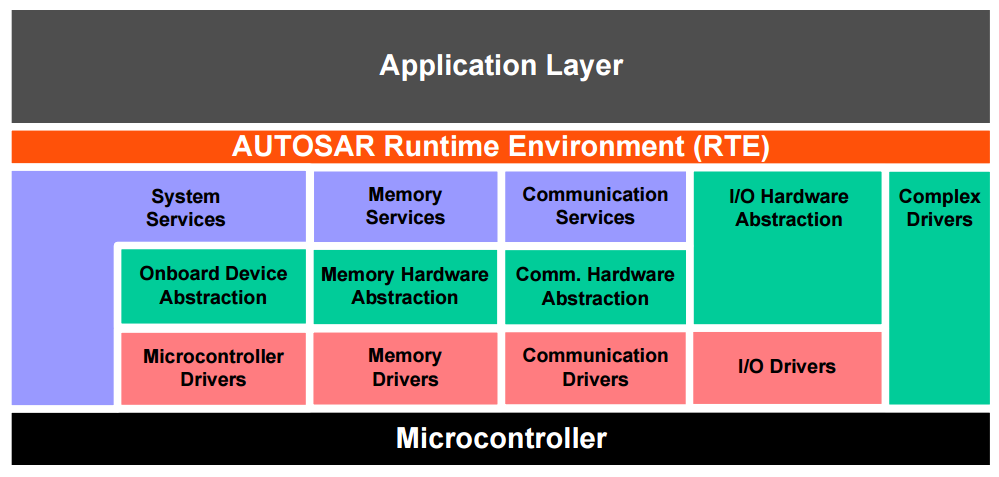
\includegraphics[scale=0.35]{content/images/autosararch.png}
	\caption{AUTOSAR Architecture \cite{autosararch}}
	\label{fig:autosararch}
\end{figure}

\section{Parallel Design using Eclipse APP4MC} \label{app4mcchapter}
As introduced in the Introduction chapter, this work uses Eclipse APP4MC development tool for software parallelization. \textbf{APP4MC (Application Platform Project for MultiCore)} \cite{ICPDSSE} \cite{app4mcweb} is an Eclipse-based project that aims to achieve an open, consistent, expandable tool platform for embedded software engineering \cite{app4mchelp}. APP4MC targets multi-core and many-core platforms, while the main focus is the optimization of embedded multi-core systems \cite{app4mchelp}. Due to its focus, APP4MC is partnered with many automotive OEMs and part suppliers that deal with embedded software engineering.  Furthermore, it supports interoperability and extensibility and unifies data exchange in cross-organizational projects \cite{app4mcweb}. Additionaly, since APP4MC uses Eclipse platform to its purposes, the development environment has a complete open-source nature under Eclipse Public License (EPL) \cite{epl}. 

%xxxx
Eclipse APP4MC platform editor window can be seen in the Figure \ref{fig:app4mcenv} \cite{app4mchelp}. In the figure, Explorer window is used for finding models, performing operations such as partitioning, task generation, mapping, and model migration. The tree editor shows the hierarchical structure of the selected AMALTHEA model, whereas the Element Properties window is used for editing the properties of AMALTHEA model elements selected in the Tree Editor \cite{app4mchelp}.

\begin{figure}[!ht]
	\centering
	\captionsetup{justification=centering}
	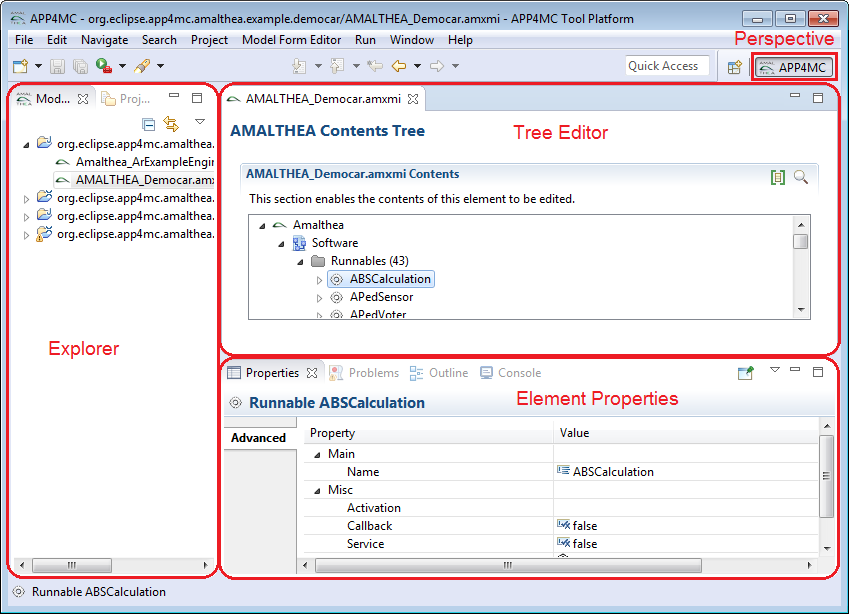
\includegraphics[width=\textwidth]{content/images/app4mcenv.png}
	\caption{Eclipse APP4MC platform Editor Window \cite{app4mchelp}}
	\label{fig:app4mcenv}
\end{figure}


APP4MC is a project that has a lot of synergies with its predecessor AMALTHEA4public \cite{amalthea4publicweb} project. APP4MC uses AMALTHEA models, which are XML models that describe software components and hardware platforms. Main operation of APP4MC involves modeling the system by creating AMALTHEA models and performing partitioning, mapping, optimization on parallel programs \cite{ICPDSSE}. APP4MC also has the ability to trace simulate parallel programs. Basic ingredients for an AMALTHEA model is illustrated in the Figure \ref{fig:app4mcmodel} \cite{app4mcweb}. It is seen that AMALTHEA model can contain software decisions, costs, constraints, as well it can contain hardware platform information \cite{app4mcweb}. Constraint models are used to define process groups to make sure some processes belong together. Furthermore, a target platform dependency of a process group is also modeled using constraints model. More information on modeling will be discussed later in this section.

\begin{figure}[!ht]
	\centering
	\captionsetup{justification=centering}
	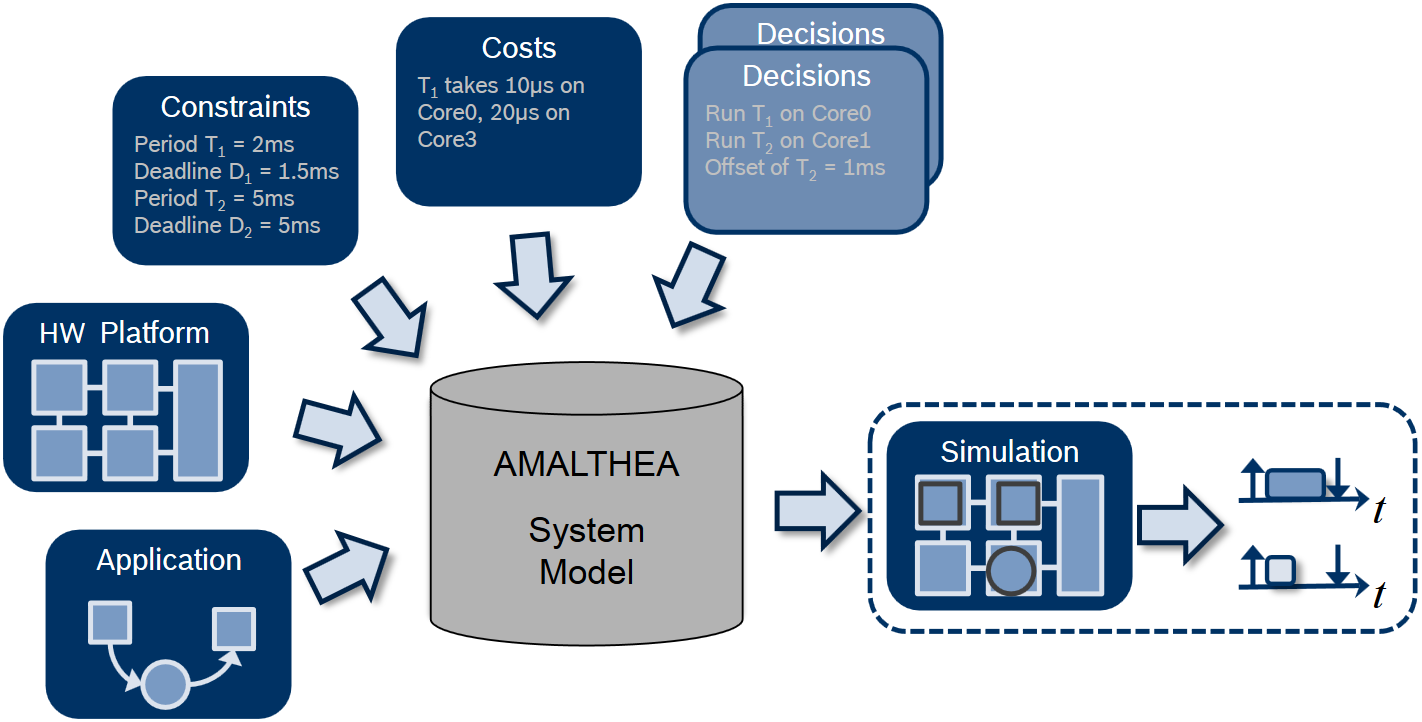
\includegraphics[width=\textwidth]{content/images/app4mcmodel.png}
	\caption{AMALTHEA Model for APP4MC \cite{app4mcweb}}
	\label{fig:app4mcmodel}
\end{figure}

An illustration of how parallel software can be designed for embedded multi-core platforms are given in the Figure \ref{fig:app4mcdesign}. Studying the illustration given in the Figure \ref{fig:app4mcdesign} in combination with the parallel design techniques that were given in the Section \ref{designtech}, the following remarks can be made regarding the design procedure with APP4MC platform:
\begin{itemize}
	\item \textbf{Modeling:} Design of a parallel software starts with modeling in APP4MC. An AMALTHEA model is constructed that involves three seperate models: (1)- hardware model, (2)-software model, (3)-constraints model. In the hardware model, each distributed ECU is modeled in a hierarchical  manner. Hardware model involves information such as number of processor cores, system clock frequency for processors, and memory details. In the software model, runnables are modeled. Runnables are found with the help of binary analysis tools and by using the decomposition technique mentioned in the Section \ref{designtech}. Each runnable are modeled by making use of information such as granularity (number of instructions) and label accesses (memory read-write). In the early development stages, model contains a rough model of the software, but the model is constantly improved by using the Tracing functionality of the APP4MC as well it can be improved by using several other tracing software.
	\item \textbf{Partitioning:} Partitioning stage in APP4MC-aided parallel design corresponds to identification of initial tasks. After an initial AMALTHEA model is constructed, the one can perform partitioning in APP4MC by simply selecting the model and pressing the "Perform Partitioning" button. At this stage, APP4MC will analyze the runnables and runnable label accesses in order to suggest how tasks should look like for a balanced parallel distribution. APP4MC uses two partitioning algorithms that are ESSP (Earliest Start Schedule Partitioning) (performed by default) and CPP (Critical Path Partitioning) in order to find the partitions of the system. ESSP and CPP algorithms are based on the Graph Theory \cite{graphtheory} which is commonly used in hardware and software co-design. Partitioning algorithms are used for analysis of the granularity and communication costs of individual runnables and create best possible parallelized partitions.
	\item \textbf{Task Generation:} Initial tasks (partitions) are finalized by pressing "Generate Tasks" button. By making use of the dependencies between partitions and by grouping them, APP4MC generates a model that contains the desired amount of tasks with the help of "Task Generation" phase. 
	\item \textbf{Mapping (with Simulation and Optimization):} As known, mapping is the stage of placing the software distributions (tasks, processes, threads) into the processors. By making use of the hardware capabilities and using optimization strategies (such as Integer Linear Programming), APP4MC is able to find a mapping model of the system. The utilization details of the simulations will be seen at the end of the mapping stage.
	\item \textbf{Code Generation:} Since APP4MC provides model-based development, code generation features for C language are available. If desired, APP4MC generates tasks that are written in C language by using the AMALTHEA system model.
	\item \textbf{Tracing:} By making use of binary tracing, AMALTHEA trace model can be observed and can be re-used to update the system model.
\end{itemize}

\begin{figure}[!ht]
	\centering
	\captionsetup{justification=centering}
	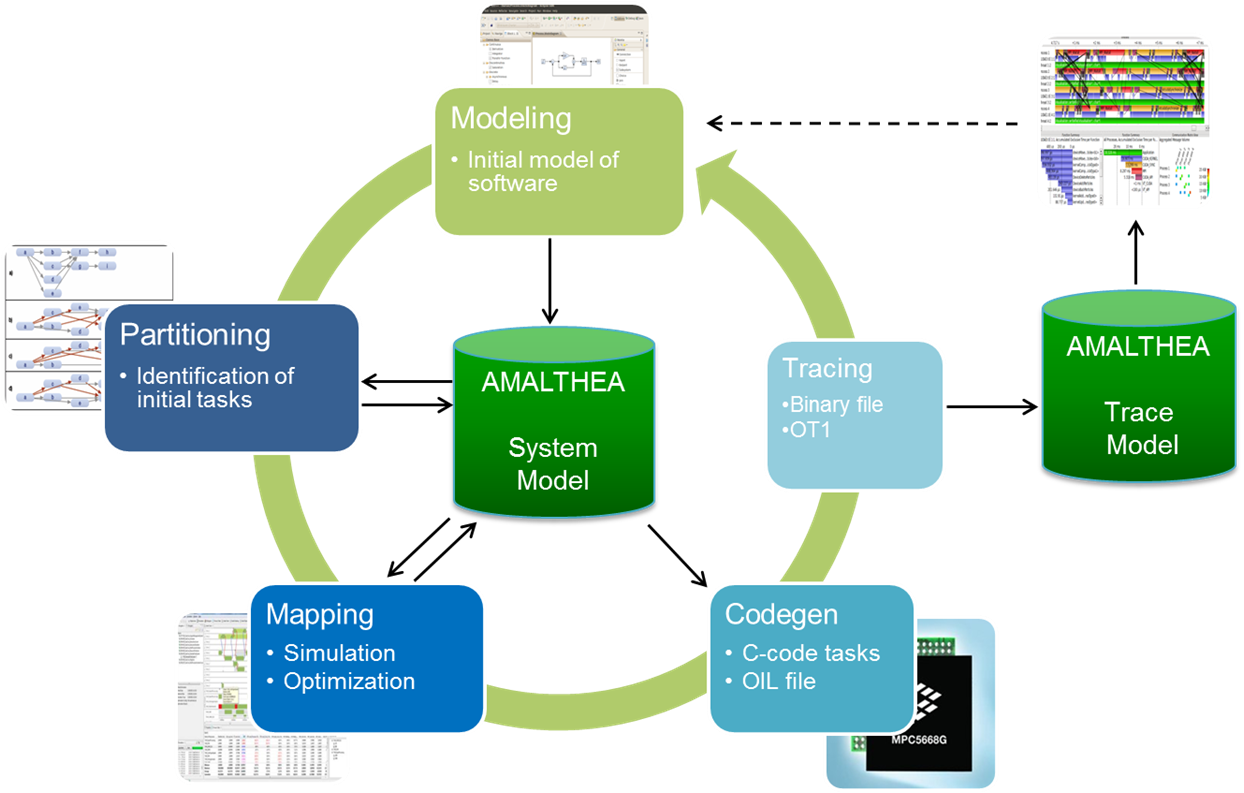
\includegraphics[width=\textwidth]{content/images/app4mcdesign.png}
	\caption{Illustration of how parallel software are designed using APP4MC platform \cite{amalthea4publicweb}}
	\label{fig:app4mcdesign}
\end{figure}
%final remarks, objectives, usefulness, ve...
%model and results will be discussed in the results section.
APP4MC promises beneficial set of tools for embedded parallel software development. However, the demonstration of its features is needed for further improvement. Therefore, in this work APP4MC is used for system parallelization for A4MCAR, a demonstrator RC-Car. Further sections will involve design, modeling, and evaluation of software distributions for this demonstrator.

%arayuz - once de bahsedilebilir...

%partitioning den de bahsedilecek ESSP falan..
%optimization algoritmasindan da bahsedilecek ILP...
%Introduction} %Motivation, why is it useful...
%Features} %include schema
%Modeling}

%Theoretical Objectives, Practical Objectives and 
\section{Related Work}
Some text will come here! \\

%%% CHAPTER A4MCAR ----------------------------------begin----
\chapter{Distributed Multi-core Demonstrator (A4MCAR) Design and Implementation} \label{designchapter}
\section{System Overview}
As introduced in the Chapter \ref{introductionchapter}, A4MCAR is a demonstrator RC-Car for the APP4MC development environment. A4MCAR provides a distributed multi-core architecture that allows the demonstration of embedded low-level and high-level applications. Pictures of the A4MCAR can be seen in Figure \ref{fig:a4mcar}.
\begin{figure}[!ht]
	\centering
	\captionsetup{justification=centering}
	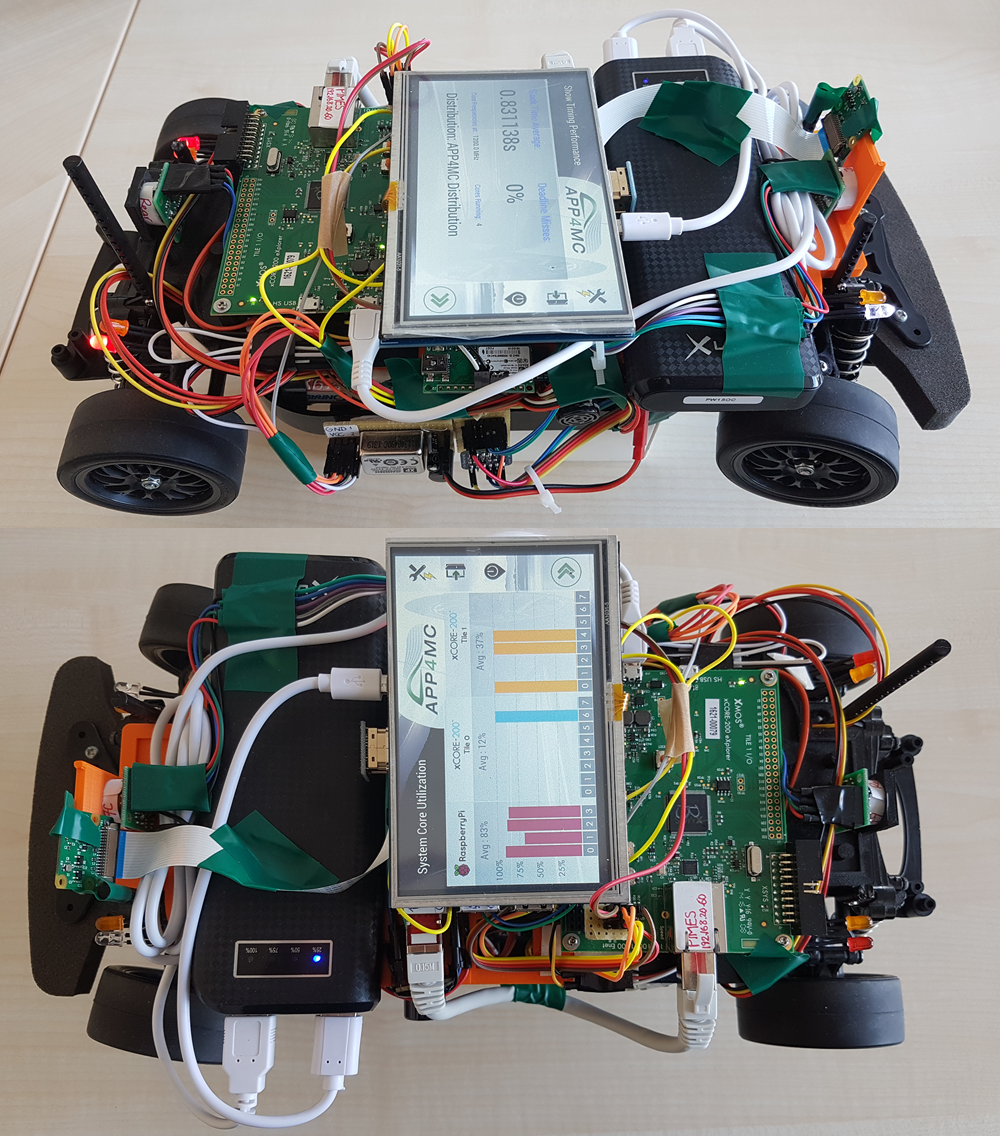
\includegraphics[scale=0.4]{content/images/a4mcar.png}
	\caption{A4MCAR}
	\label{fig:a4mcar}
\end{figure}
\subsection{System Features}
As A4MCAR targets automotive industry and parallelization studies done by APP4MC, it features not only sensing and actuation related features but also applications that would help with task to core distributions and parallelization performance evaluation. One could see the featured applications for the A4MCAR in Figure \ref{fig:tasksoverall}. 
\begin{figure}[!ht]
	\centering
	\captionsetup{justification=centering}
	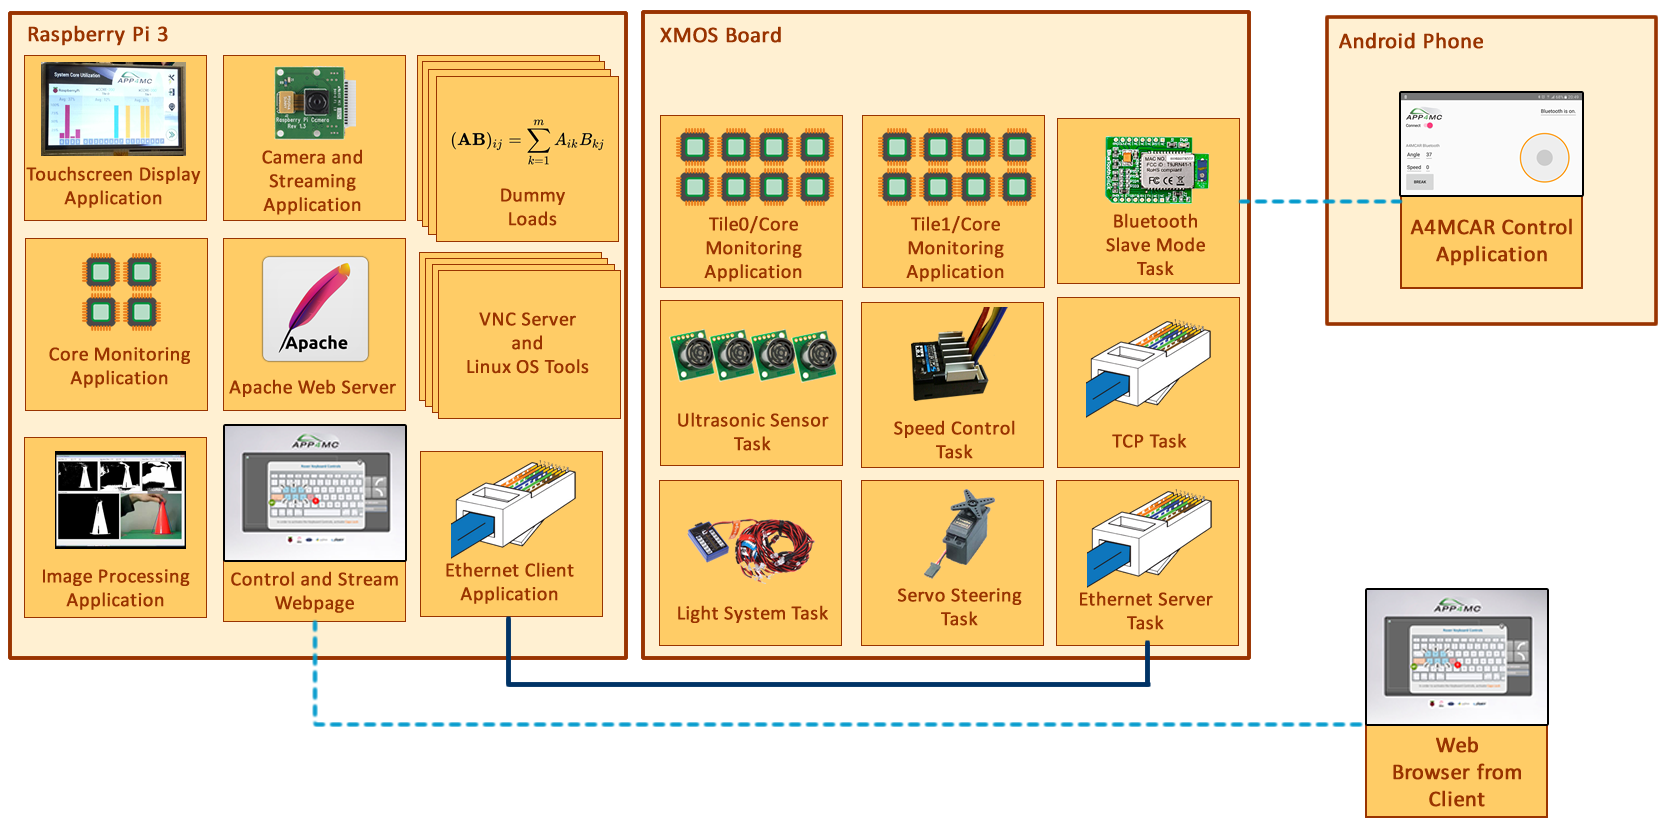
\includegraphics[scale=0.3]{content/images/tasksoverall.png}
	\caption{Applications developed and/or maintained for A4MCAR}
	\label{fig:tasksoverall}
\end{figure}
In the figure, it is seen that the low level module of A4MCAR, built using xCore-200 eXplorerKIT targets mostly actuation and sensing related applications. The full list of tasks developed for the low-level module includes:
\begin{itemize}
	\item Core monitoring applications for each tile (two exist) that calculates the average core usages.
	\item Bluetooth task to configure bluetooth module in slave mode and receive data over UART interface.
	\item Proximity measurement task that obtaines the distance sensor information from four SR-04 sensors over an I2C sensor network.
	\item Speed control task in order to use PWM to drive speed controlling motor.
	\item Steering task that controls a servo motor using PWM signaling in order to steer the A4MCAR using external inputs.
	\item Light system task in order to control a light module for certain conditions.
	\item Ethernet server task to maintain a TCP server for data reception and transmission from high level module.
	\item TCP task and several other ethernet configuration related tasks to configure ethernet module (PHY) drivers and establish proper TCP connection.
\end{itemize}
In order to investigate parallelization outcomes on Real-time Linux and make use of high level features such as web server, image processing and touchscreen interface high-level module is introduced to the system. High-level module is designed so that it can communicate with low-level module over TCP in order to send driving information and retrieve core information from low-level module. It is important to mention that high-level module uses Raspberry Pi 3 in order to achieve high level tasks using a robust Debian-based OS, namely Raspbian. Although the features of the high-level module is illustrated in the Figure \ref{fig:tasksoverall}, full feature list can be given as follows:
%xxxxxxxxxxxxxxxx
\begin{itemize}
	\item Core monitoring application that calculates the average core usages on each core.
	\item Image processing application that helps to find a traffic cone.
	\item Apache Web Server that is used to host a web page which shows average core usage, show Raspberry Pi 3 camera (Raspicam) stream and helps to drive the A4MCAR via web page controls.
	\item Ethernet client application that writes handles data transmission and reception to and from server using file operations and data parsing.
	\item Camera and streaming application that starts the Raspicam and maintains the stream using configuration parameters such as resolution, quality, frame rate, port and etc.
	\item A webpage which is used for driving the A4MCAR as well as display core usages on each core and Raspicam stream.
	\item A touchscreen display application which is used for displaying all cores and their utilization, starting and killing all applications on high-level module, allocation of processes on high-level module to cores dynamically, visualization of timing related performance indicators such as average slack time and deadline misses percentage, selecting different distributions, and configuration of the IP addresses on high-level module.
	\item Dummy load processes that perform random matrix multiplication in order to find performance indicators in full utilization.
	\item Several Linux processes that run Linux OS kernel and VNC server process that provides PC connection via SSH connection.
\end{itemize}
\subsection{Infrastructure}  %x XMOS and Rpi: boards, (inkl. board pictures) processors, memory, languages, compilers, infrastructure
Processing infrastructure of the A4MCAR is divided into two modules: Low-level module and high-level module. Low-level module uses a multi-core development kit XMOS xCore-200 eXplorerKIT, whereas high-level module uses a Raspberry Pi 3 which are both shown in Figure \ref{fig:boards}.
\begin{figure}[!ht]
	\centering
	\captionsetup{justification=centering}
	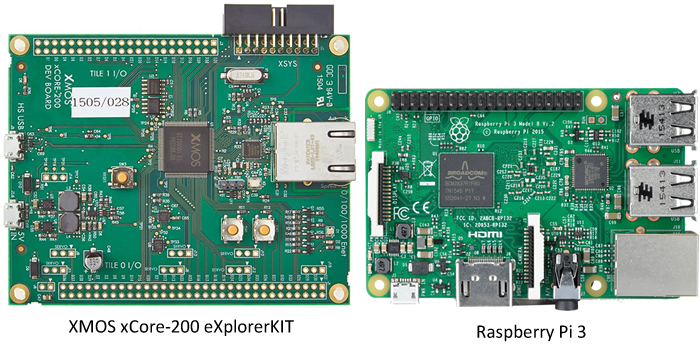
\includegraphics[scale=0.6]{content/images/boards.jpg}
	\caption{Development boards used in A4MCAR}
	\label{fig:boards}
\end{figure}

\subsubsection{Low-level Infrastructure} \label{lowlevelmoduleinfra}
XMOS xCore-200 eXplorerKIT features XEF216-512, a powerful multi-core microcontroller that provides sixteen 32-bit logical cores that are divided into tiles \cite{xmoskitweb}, which are identical units that contain processing unit, cache memory and switch mechanism \cite{tileref}. XMOS xCore-200 eXplorerKIT contains two tiles with eight logical cores in each tile. It is important to add that logical cores of eXplorerKIT provides 2000 MIPS (Million Instructions per Second) processing power and 512 KB SRAM along with up to 500 MHz clock speed. The specified performance values are considered to be relatively powerful compared to regular microcontrollers. While the processing power and cache memory of its two tiles are identical, ports on each tile have access to different peripherals located on the board. With 53 high-performance GPIO, XMOS xCore-200 eXplorerKIT features 100/1000Mbps Ethernet module, high speed USB interface, a 3D accelerometer, a 3-axis gyroscope, and six servo interfaces which makes the kit useful in a wide variety of applications that include robotics, automotive, signal processing and communication applications \cite{xmoskitweb}.

As the name of the development kit suggests, XEF216-512 uses XMOS' xCore-200 architecture. An illustration of xCore-200 architecture is given in Figure \ref{fig:XE216Architecture}.
\begin{figure}[!ht]
	\centering
	\captionsetup{justification=centering}
	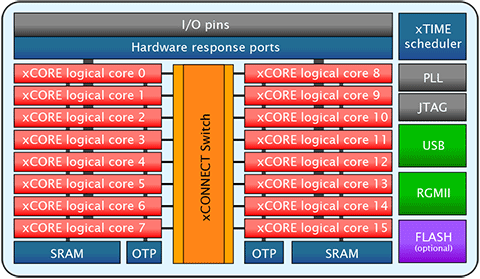
\includegraphics[scale=0.7]{content/images/XE216Architecture.png}
	\caption{Illustration of XMOS' xCore-200 Architecture \cite{xmosflyer}}
	\label{fig:XE216Architecture}
\end{figure}

In xCORE-200 architecture, each core uses the memory of the tile it belongs to and logical cores communicate using a high-speed network. Thus, channels which achieve task communication are linked to other cores via \textbf{xCONNECT Switch}. While this is the case for tasks that are distributed to seperate cores, for tasks that are placed in the same core \textbf{xTIME Scheduler} automatically schedules tasks by synchronizing events. The xTIME Scheduler works similar to RTOS in traditional microcontrollers and uses \textbf{Round-robin scheduling method} \cite{xmosdatasheet} \cite{roundrobin} which is a simple and starvation-free scheduling technique that gives each task equal time slices and disregards priorities in order to schedule processes or tasks. Round-robin scheduling is widely used in operating systems \cite{roundrobin}.

In xCORE architecture, the synchronization of task communication is handled by events rather than ISRs (Interrupt Service Routines) as compared to a traditional microcontroller. Each xCORE tile is connected to hardware ports and thereby pins which can be driven high and low in order to drive electrical peripherals. xCORE tiles are also connected to an OTP (One Time Programmable Memory) and SRAM (Static Random Access Memory). While OTP is used for code locking features, SRAM serves as a memory where the instructions and variables are located \cite{xmosdatasheet}.

Since the xCORE features multiple cores unlike a traditional microcontroller, it should be clearly understood that the task interruption is not present in xCORE. This is illustrated delicately in the Figure \ref{fig:xmosvstraditional} \cite{xmosflyer}. If not stated otherwise in an xCORE application, all the tasks are placed to different logical cores. This means that all the tasks are executed completely parallel in hardware. When the tasks are shared in a core, then the multi-tasking features of the XMOS are invoked and parallelized just like in an RTOS from traditional microcontrollers \cite{xmosflyer}.
\begin{figure}[!ht]
	\centering
	\captionsetup{justification=centering}
	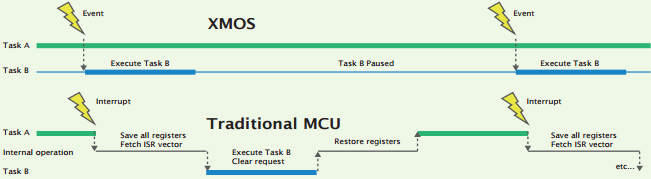
\includegraphics[width=\textwidth]{content/images/xmosvstraditional.png}
	\caption{XMOS vs Traditional Microcontroller \cite{xmosflyer}}
	\label{fig:xmosvstraditional}
\end{figure}

Most of the traditional microcontrollers including xCORE microcontrollers nowadays feature pipelining mechanism. The \textbf{instruction pipeline} is a set of data processing elements connected in series, where the output of one element is the input of the next one \cite{pipelinebook}. Via instruction pipelining, processors make use of the stages in order to use the clock to its full performance to reduce the time taken to execute instructions. This mechanism is also present in most of the XMOS processors with five stages. How instruction pipelining mechanism achieves faster instruction execution is illustrated in the Figure \ref{fig:pipeline} \cite{xmosflyer}.
\begin{figure}[!ht]
	\centering
	\captionsetup{justification=centering}
	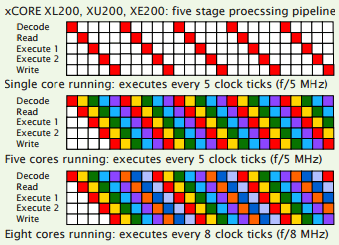
\includegraphics[scale=0.9]{content/images/pipeline.png}
	\caption{Pipelining Explained on XMOS \cite{xmosflyer}}
	\label{fig:pipeline}
\end{figure}

Traditionally, XMOS based microcontrollers are programmed via xTimeComposer, which is an Eclipse-based software development platform for XMOS based multi core microcontrollers with integrated features such as simulation, symbolic debugging, tracing, runtime instrumentation, and timing analysis with a static code timing analyzer called \textbf{XTA}\cite{xmosflyer}. As A4MCAR needs to make use of timing and performance values, some tracing tools and XTA has been widely used during the development. xTIMEComposer development environment windows are shown and illustrated in Figure \ref{fig:xtimecomposerwindows}.
\begin{figure}[!ht]
	\centering
	\captionsetup{justification=centering}
	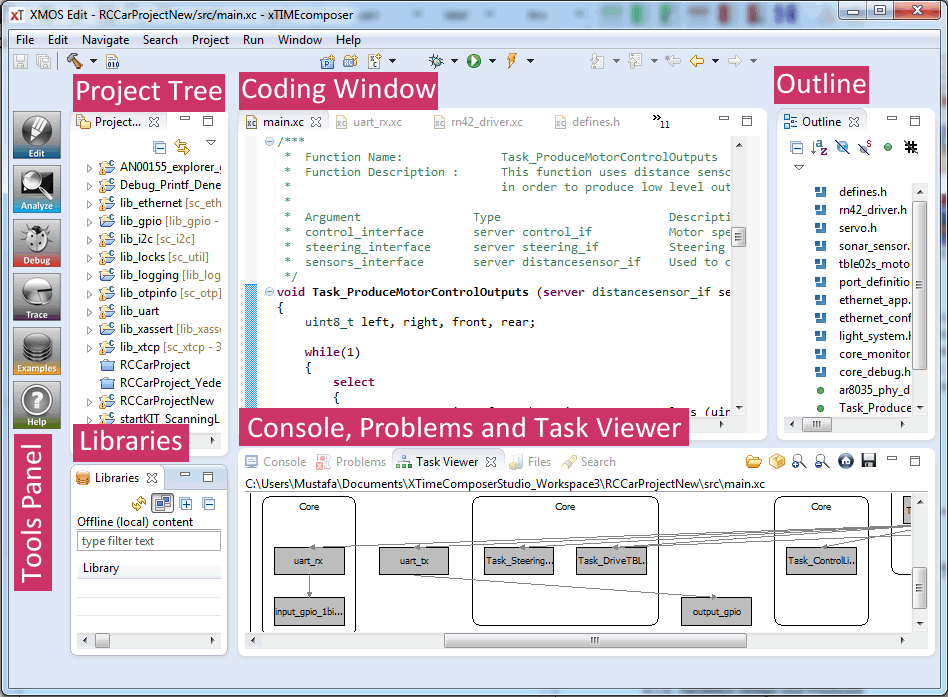
\includegraphics[scale=0.5]{content/images/xtimecomposerwindows.png}
	\caption{xTIMEComposer 14.2.3 Development Environment Windows}
	\label{fig:xtimecomposerwindows}
\end{figure} \\
%Explain the fucking composer
In the Figure \ref{fig:xtimecomposerwindows} it is seen that the main development environment consists of the following windows:
\begin{itemize}
	\item \textbf{Project Tree:} This window is used for managing projects and source, include, binary and configuration files within projects.
	\item \textbf{Coding Window:} Coding window is used for writing code and placing breakpoints. One can switch between several files by clicking on the tabs located on the top of this window.
	\item \textbf{Console:} The console is used for viewing the building process, verbose and debugging information.
	\item \textbf{Problems:} The problems window is used for seeing warnings and errors that result from the code.
	\item \textbf{Task Viewer:} The task viewer is a special feature that is unique in xTIMEComposer and it is used to visualize tasks and at which core and tile they are located. The channel and interface connections between tasks are also visualized using this window.
	\item \textbf{Tools Panel:} This window is used in order to switch between several tools that xTIMEComposer provide. Analyze and Debug tools are widely used in development. Analyze tool opens xTIMEComposer Timing Analyzer (XTA) tool whereas Debug tool is used for traditional debugging using breakpoints.
	\item \textbf{Outline:} Outline window lays out the main elements of a file such as its includes, tasks, objects and so on.
	\item \textbf{Libraries:} The Libraries window can be used in order to search offline and online libraries.
\end{itemize}
%files in a project.. configuration..
%\begin{figure}[!ht]
%	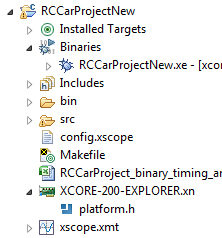
\includegraphics[scale=0.9]{content/images/xtimeprojecttree.jpg}
%	\caption{Files in a xTIMEComposer project}
%	\label{fig:xtimeprojecttree}
%\end{figure}
%languages
Programming languages which are used for xCORE processors can be listed as C, C++ and xC (C with multicore extensions) \cite{xmosdatasheet}. The aforementioned xC language features three main keywords in order to represent task communication. To represent an interface that sends data to another task, \textbf{client} keyword is used whereas if a task is retrieving data from one or many client ports, the receiving interface is named \textbf{server}. It is important to mention that server interface receives data by throwing events. Additionally, xC also allows to define function attributes which are \textbf{combinable} and \textbf{distributable}. XMOS Programming Guide \cite{xmosprogrguide} suggests that combinable tasks are the ones that continuously react to events and they can be combined to have several tasks running on the same logical core. It is added in the XMOS Programming Guide \cite{xmosprogrguide} that distributable tasks are not dedicated to only one logical core but they run when required by the tasks connected to them. Furthermore, xC features \textbf{timers}, \textbf{events}, \textbf{guards}, \textbf{event priority ordering} in order to help us develop event-based software. These features of xC make multi-core programming easy and robust on xCORE processors.

\subsubsection{High-level Infrastructure} \label{hlinfrasection}
%xxxxxxxxxxxxxxxx
High-level processing unit of A4MCAR, Raspberry Pi 3, is a widely used single board computer in embedded applications. It has 1.2GHz 64-bit quad-core processor with ARMv8 architecture, 1GB of RAM, VideoCore IV 3D graphics core and several interfaces such as 40 GPIO pins, 4 USB ports, HDMI port, ethernet port, audio jack, camera interface (CSI), display interface (DSI), micro SD card slot \cite{raspberrypiinfo}. The reason Raspberry Pi 3 is preferred in embedded systems applications is that it provides excellent connectivity via 802.11n Wireless LAN module, Bluetooth 4.1 module, and Bluetooth Low Energy (BLE) module. 

Raspberry Pi 3 can be booted with modern Linux-based operating system distributions such as Debian-based Raspbian OS \cite{raspbiandownload} and Ubuntu-based Ubuntu MATE\cite{ubuntumatedownload} \cite{raspberrypiinfo}. It should be noted that in A4MCAR, Raspbian OS has been used due to its wide software repository and driver support. The fact that Raspberry Pi 3 functions as a Linux computer helps in developing high-level applications that require operating system presence. The open-source nature of Linux and its software ecosystem provides flexible and traceable software development. In A4MCAR, the traceability and flexibility features of Raspberry Pi 3 are highly used. Furthermore, a wide variety of programming languages such as C, C++, Java, LISP, Python, Bash, Perl etc. are supported in Raspberry Pi. In A4MCAR, programming languages such as C, C++, Python, Bash, HTML, JavaScript has been used in order to develop high-level module.

A brief explanation of the architecture of Linux-based computers and as an extension the architecture of the Raspberry Pi 3 should be given in order to develop applications and understand how applications running on Linux work. With that idea in mind, high-level overview of the structure of  the \textbf{Linux kernel} and high-level layers in a Linux system which is given in Figure \ref{fig:linuxarchitecture} should be considered \cite{linuxkernelbook}.
\begin{figure}[!ht]
	\centering
	\captionsetup{justification=centering}
	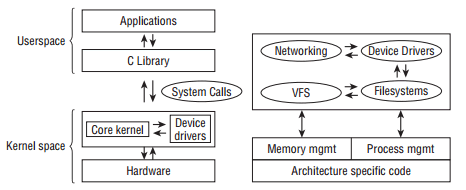
\includegraphics[scale=0.9]{content/images/linuxarchitecture.png}
	\caption{High-level Linux system architecture \cite{linuxkernelbook}}
	\label{fig:linuxarchitecture}
\end{figure}

According to Mauerer \cite{linuxkernelbook}, the kernel is the intermediary level between the hardware and the software that addresses the devices and the components of the system (such as CPU, memory and I/O devices) by passing application requests. While kernel processes requests from user applications, it makes its own decision where data is located and which commands to send to hardware. Kernel is also the instance in a Linux system which shares available resources such as CPU, memory, and network; which is why it should be addressed while working with parallel applications.

In the figure, it is seen that kernel space is not only responsible for accessing device drivers, but it is also responsible for memory and process management. A program under Unix systems (such as Linux) that run continuously is referred to as \textbf{processes} and they are scheduled by Linux kernel. The multi-tasking of processes are done by a mechanism that is called \textbf{task-switching} or \textbf{context-switching} and this is achieved to ensure that CPU performs according to the scheduled tasks. The concept of \textbf{scheduling} in a Linux system is also handled by kernel and it is the procedure of deciding how CPU time should be shared between existing processes. Additionally, \textbf{threads} in a Linux-based computer system are also big parts of multi-tasking which are also handled by kernel. Threads share the same data and resources but they have different execution paths through program \cite{linuxkernelbook}.

In A4MCAR high-level module, we mostly deal with processes and investigate ways to efficiently parallelize process-based system. In this regard, it is crucial to understand the process life cycle and how kernel schedules processes. This knowledge is described delicately by Mauerer \cite{linuxkernelbook} and Ward \cite{howlinuxworksbook}. Figure in \ref{fig:processlifecycle} depicts an illustration of how process life cycle works \cite{linuxkernelbook}.
\begin{figure}[!ht]
	\centering
	\captionsetup{justification=centering}
	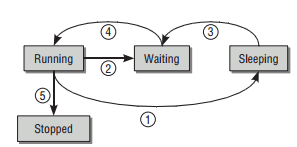
\includegraphics[scale=1]{content/images/processlifecycle.png}
	\caption{Process Life Cycle in a Linux System \cite{linuxkernelbook}}
	\label{fig:processlifecycle}
\end{figure}

% process life cycle explain..
In Figure \ref{fig:processlifecycle}, state machine for processes in a Linux system is given. The states of processes can be listed as Running, Waiting, Sleeping, and Stopped. These states can be explained using following scenerios \cite{linuxkernelbook}:
\begin{itemize}
	\item If the process is being currently executed, process is in \textbf{Running} state.
	\item If the process is not being executed because it is waiting for CPU to finish executing another process, it is in \textbf{Waiting} state.
	\item If the process is waiting for an external event such as a periodic activation or a sporadic activation, it is in \textbf{Sleeping} state. Notice that transition from Sleeping state to Running state is not possible. A process switches to Waiting state from Sleeping state in order to wait for current process to finish its execution.
	\item If the user decides to kill (terminate) the application, the process goes into \textbf{Stopped} state.
	\item If a process has been killed but its entries are still alive in the process table, the state of that process is called \textbf{Zombie}. Therefore, although not shown, transition from Running state to Zombie state is also possible.
\end{itemize}

It is important to note that these states are traceable using Linux kernel access methods which will be explained in Chapter \ref{informationchapter} of this report along with several other Linux kernel concepts.

% terminal, compilers, Nano, Vi, Emacs
Raspberry Pi is conventionally programmed through Linux shell which is programmed and commanded with the help of Bash scripting language. There are several editors and compilers introduced for Linux shell in order to help developers write, compile, debug, and trace their applications. Most popular editors involve Nano, Vi, and Emacs which are editors that can run without GNU Graphical User Interface. An alternative way is to use open-source platforms such as Eclipse with correct extensions and plugins. The conventional and standart C compiler for the Unix platform GCC, and the standart Python shell can be accessed using all these compilers. For the sake of demonstration, the Linux shell which is running Emacs is shown in the Figure \ref{fig:linuxeditors}. It is important to note that in the development of A4MCAR, Nano and Emacs editors have been frequently used as Nano provides easiest way to interact with Linux shell and Emacs provides advanced features to compile and debug programs rapidly.
\begin{figure}[!ht]
	\centering
	\captionsetup{justification=centering}
	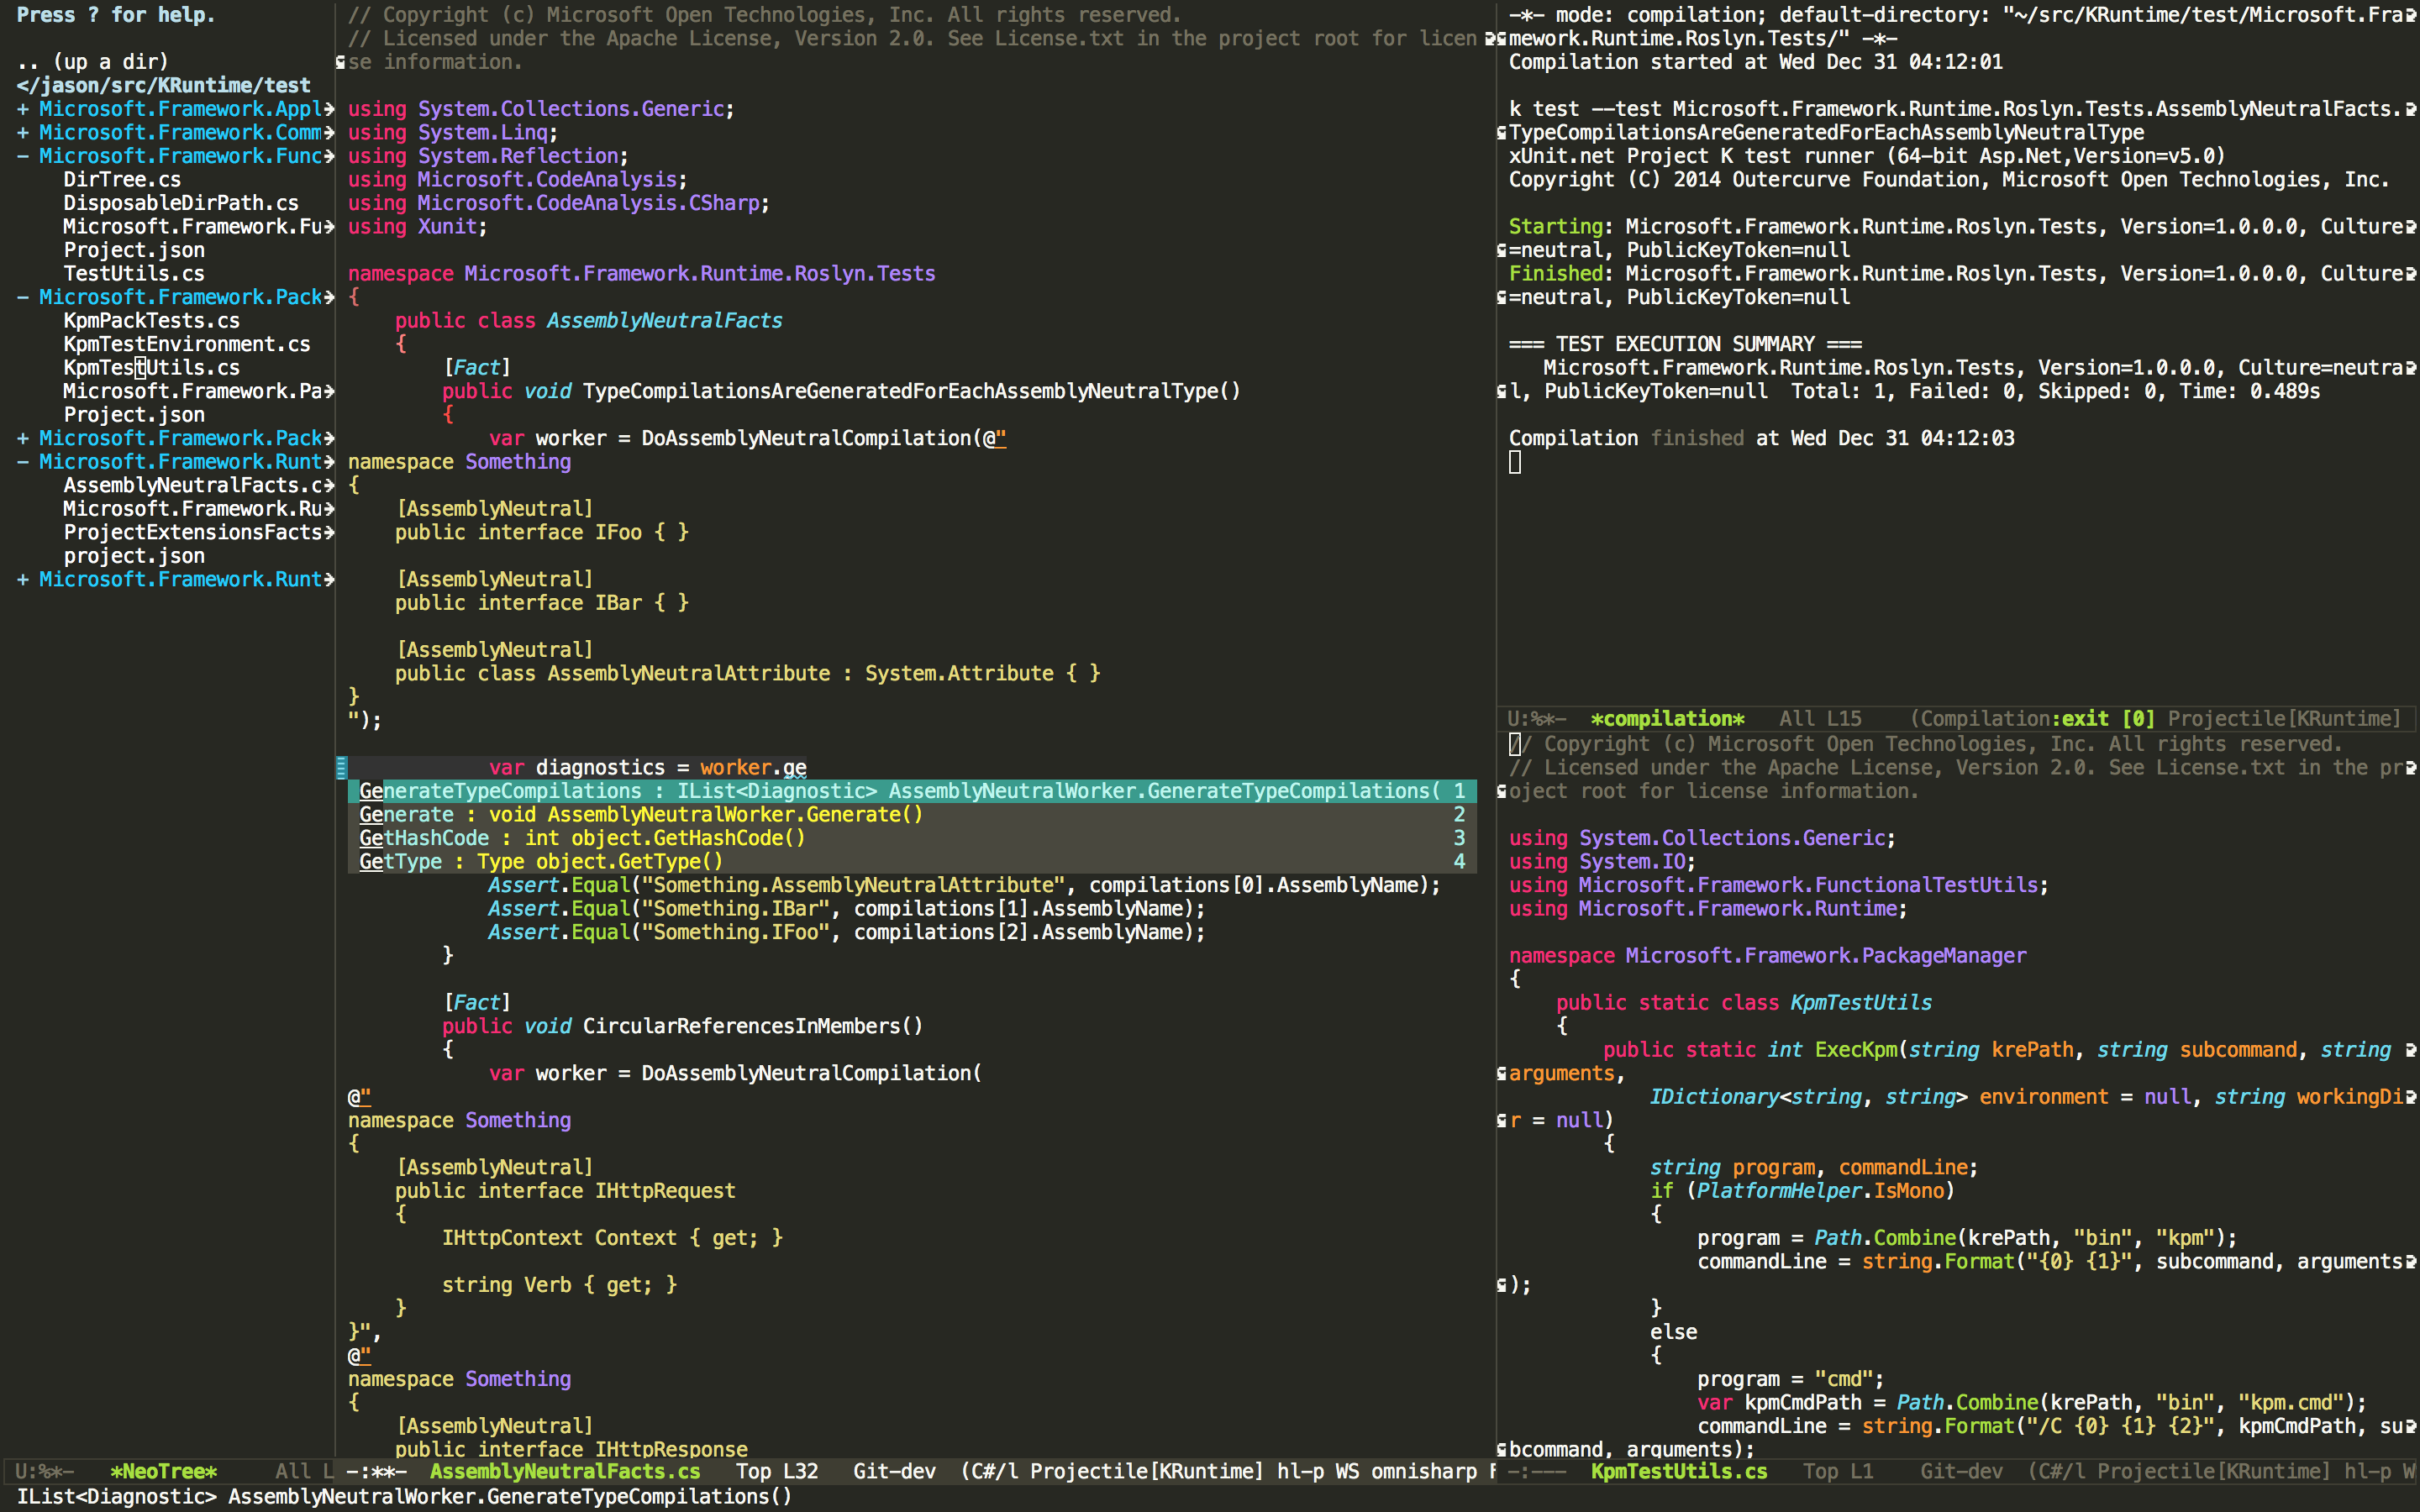
\includegraphics[width=\textwidth]{content/images/linuxeditors.png}
	\caption{Linux Shell running Emacs}
	\label{fig:linuxeditors}
\end{figure}
%Raspbery Pi stuff here!
\subsection{Hardware Design, Sensors and Protocols}
One should care for a robust hardware design in order to avoid having software problem and safety related issues. In A4MCAR, a number of modules have been used alongside development kits in order to provide utility to the demonstrator. On the low-level module side, a light system, an RN-42 Bluetooth module, four SRF-02 ultrasonic sensors, a servo motor, a TBLE-02S electronic speed controller have been used. The high-level module side however only is connected to a touchscreen display and a Raspicam (Raspberry Pi camera). The overview of hardware connections, used protocols and device architectures are given in the Figure \ref{fig:hwoverview}.
\begin{figure}[!ht]
	\centering
	\captionsetup{justification=centering}
	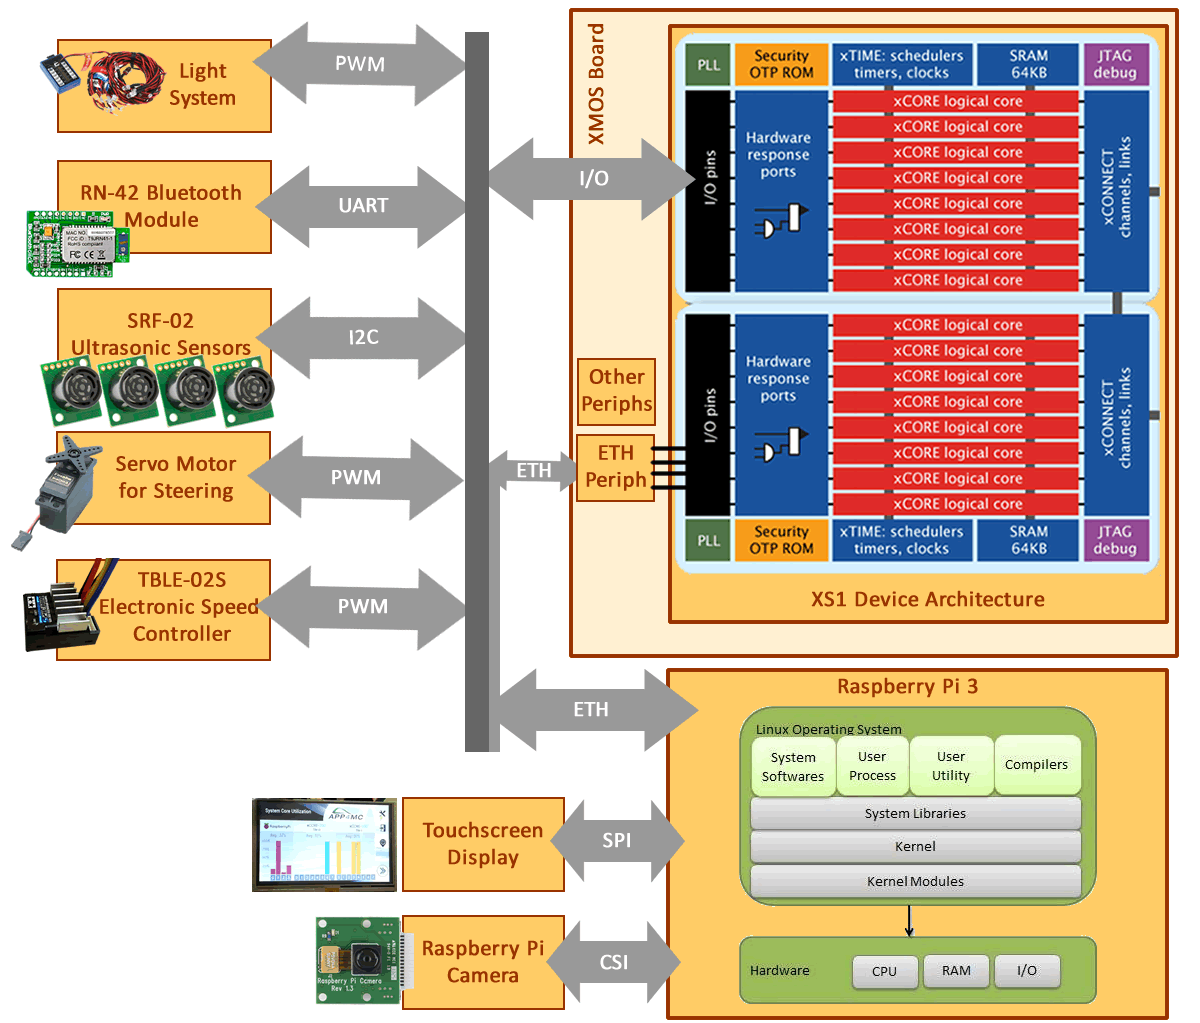
\includegraphics[width=\textwidth]{content/images/hwoverview.png}
	\caption{Hardware overview of A4MCAR}
	\label{fig:hwoverview}
\end{figure}

The system uses various communication protocols, seen in Figure \ref{fig:hwoverview} in order to interact with sensors, actuators and utility devices. The communication protocols and associated devices used in A4MCAR could be listed as follows:
\begin{itemize}
	\item \textbf{PWM:} In order to interact with servo motor, TBLE-02S electronic speed controller, and light system, Pulse Width Modulation (PWM) have been used. PWM is a type of modulated digital signal used mostly in control applications \cite{pwm}. By describing how much a signal is high and low with respect to time, duty cycle is measured which is given in percentage. One could observe the signal illustration given in \ref{fig:pwm} to see how commonly used duty cycles look like. In a control circuitry, by achieving various duty cycles, dimming a light or controlling the direction or speed of a motor is possible \cite{pwm}.
	\begin{figure}[!ht]
		\centering
		\captionsetup{justification=centering}
		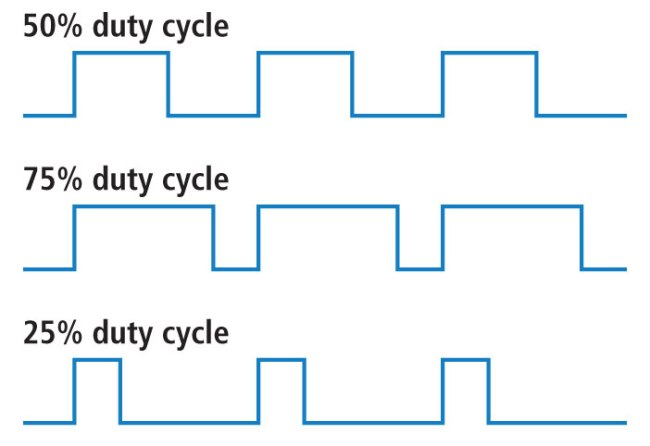
\includegraphics[scale=0.5]{content/images/pwm.jpg}
		\caption{Duty cycle example in pulse width modulation \cite{pwm}}
		\label{fig:pwm}
	\end{figure}
	\item \textbf{UART:} The RN-42 is a master-slave configurable bluetooth module (shown in Figure \ref{fig:hwoverview}) that is programmed using AT commands via UART. In A4MCAR, a RN-42 bluetooth module is used in order to interact with the bluetooth of Android devices. UART (Universal Asynchronous Receiver and Transmitter) is a communication protocol that achieves simple communication of two equivalent nodes. UART is a half-duplex and asynchronous serial protocol that doesn't communicate using a clock. Half-duplex nature of UART makes it so that transmitting and receiving lines can not be achieved simultaneously. It became a universal format because it is being used in telephone lines and USB ports of computers for decades. Number of bits transmitted or received per second is referred to as baud rate and it is standardized to values such as 9600, 14400, 19200, 38400, 57600, and 115200. Basic UART data packet is given in Figure \ref{fig:uartpacket}. The figure should depict that the basic format usually contains 6 to 8 data bits and start and stop bits to mark start and stop of the data packet. It should be noted that there are various formats with different sizes \cite{uart}.
	\begin{figure}[!ht]
		\centering
		\captionsetup{justification=centering}
		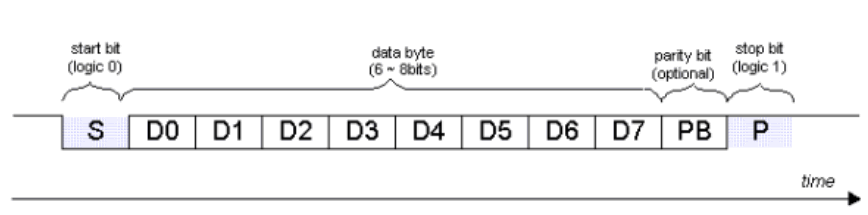
\includegraphics[scale=0.5]{content/images/uartpacket.png}
		\caption{Simple UART data packet \cite{uart}}
		\label{fig:uartpacket}
	\end{figure}
	\item \textbf{I\textsuperscript{2}C:} The proximity sensor network of A4MCAR that consists of four SRF-02 sonar sensors uses I\textsuperscript{2}C communication protocol in order to address devices in the network and obtain distance information in centimeters. I\textsuperscript{2}C (Inter integrated circuit) is a communication protocol that is intended for short distance that handles the communication of multiple slave units with one or multiple master units. Its advantage is that it uses only two wires in order to handle communication between many devices. Compared to the very similar serial communication protocol SPI, I\textsuperscript{2}C can support a multi-master system with up to 1008 slave devices. I\textsuperscript{2}C chips consist of two signals: clock signal SCL and data signal SDA. Since signals are open drain, each signal must have a pull-up resistor. The communication is handled by sending the address of the register and the data to be sent in order to write into the registers of the I\textsuperscript{2}C chips. A basic frame with 7 address bits and 8 data bits is given in \ref{fig:i2cframe} \cite{i2c}.
	\begin{figure}[!ht]
		\centering
		\captionsetup{justification=centering}
		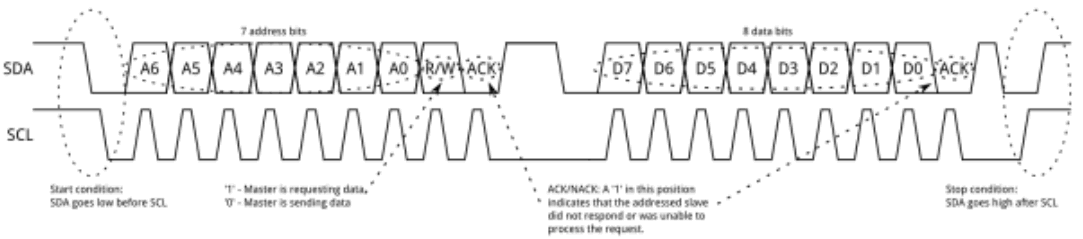
\includegraphics[scale=0.4]{content/images/i2cframe.png}
		\caption{I2C protocol frame\cite{i2c}}
		\label{fig:i2cframe}
	\end{figure}
	\item \textbf{Ethernet/TCP}: Ethernet communication using TCP (Transmission Control Protocol) is a very common method of communation that is applied within the Application, Presentation, and Session layers of the well-known OSI model. It is also a protocol that is used for high-speed data transmission to other network devices on the same network segment if used in Telnet mode. Ethernet defines two units of transmission, packet and frame. The frame includes not just the "payload" of data being transmitted but also addressing information identifying the physical "Media Access Control" (MAC) addresses of both sender and receiver, VLAN tagging and quality of service information, and error-correction information to detect problems in transmission \cite{ethernet1} \cite{ethernet2}. 
	
	In A4MCAR, a telnet server and client has been implemented using TCP protocol in order to send and receive data between high-level and low-level modules. The high-level module is configured as client, whereas low-level module is configured as the server. 
	\item \textbf{SPI}: Just like I\textsuperscript{2}C, SPI (Serial Peripheral Interface) is a communication protocol that is used to send data between processors and small devices such as sensors and displays. In SPI, MOSI, MISO, and SCK lines are available that are two data lines for each direction and a clock line. Additionally, a line of SS (Slave Select) could be used in order to select which slave device in the network is being addressd at that moment. Since SPI does only work with clock unlike the conventional UART, SPI is a synchronous communication method \cite{spi}.
	
	In A4MCAR, SPI is used by touchscreen kernel drivers in order to get touchscreen controls working. HDMI interface is also used in order to transfer media from Raspberry Pi to the Touchscreen Display.
	\item \textbf{CSI}: CSI (Camera Interface) is used by third-party applications and it is the interface that is used in order to get RaspiCam working.
\end{itemize}

In the Figure \ref{fig:RCCAR_Schematics}, the complete circuit schematics regarding A4MCAR low-level module is given. Interfacing sensors and devices should be done accordingly in order to program peripherals with xCORE-200 board properly. 
\begin{figure}[!ht]
	\centering
	\captionsetup{justification=centering}
	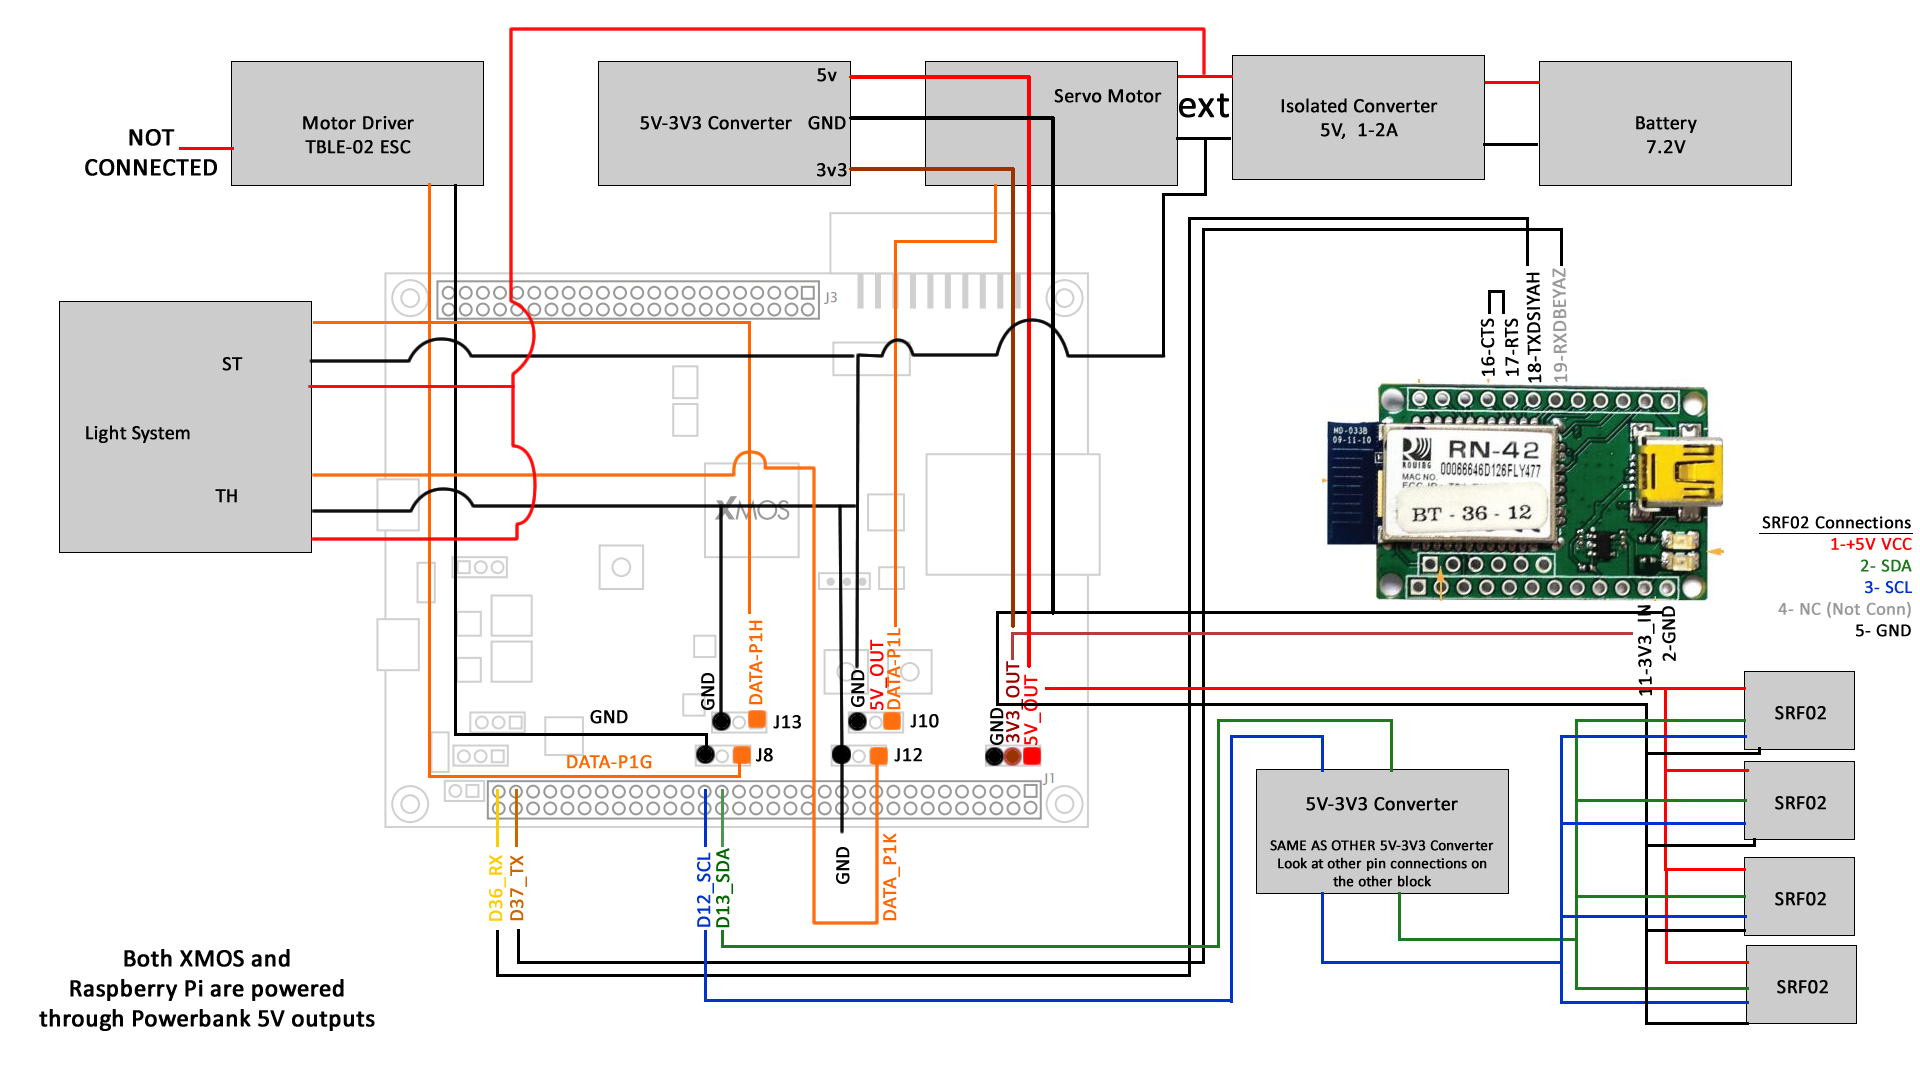
\includegraphics[width=\textwidth]{content/images/RCCAR_Schematics.png}
	\caption{Low-level module schematics of A4MCAR using XMOS xCore-200 eXplorerKIT}
	\label{fig:RCCAR_Schematics}
\end{figure}
\subsection{Safety and Power}
It should be noticed in the Figure \ref{fig:RCCAR_Schematics} there are three units that are introduced in order to get rid of the problems that are related to safety and power. To start with, since it is stated in the XS-1 architecture datasheet \cite{xmosdatasheet} that XMOS works typically with 3.3V signals and SRF-02 sensors use 5V signals \cite{srf02datasheet}, a 4-channel I\textsuperscript{2}C-safe bi-directional 5V-3.3V Logic Level Converter from Adafruit with model number BSS138 \cite{adafruitlevelconverter} has been used to convert the SDA and SCL lines of the constructed I\textsuperscript{2}C network. 

Second problem that has occurred due to low-level having multiple motors connected is the noise and excessive current drain into boards due to motors. Since that could lead to damaged development boards and chips, the solution of using two seperate power lines have been introduced. That is, using a 5V 10000mAh Powerbank to power the development boards xCORE-200 eXplorerKIT and Raspberry Pi 3 using micro-USB connectors, while using an external battery for the motors. That would reduce the noise that occurs in the signal lines since the ground lines of each battery would be isolated. In order to be on the safe side, a 5V 1A rated isolated voltage converter XP Power JCA0605S05 \cite{isolatedvoltageconverter} is also used in order to convert 7.2V battery voltage to power servo motor which is typically powered with 5V. Since datasheet of XP Power JCA0605S05 suggests that an emission circuit should be constructed, the circuit in Figure \ref{fig:emissionckt} has been constructed and printed along the isolated converter in order to meet the suggested emission level B \cite{isolatedvoltageconverter}.
\begin{figure}[!ht]
	\centering
	\captionsetup{justification=centering}
	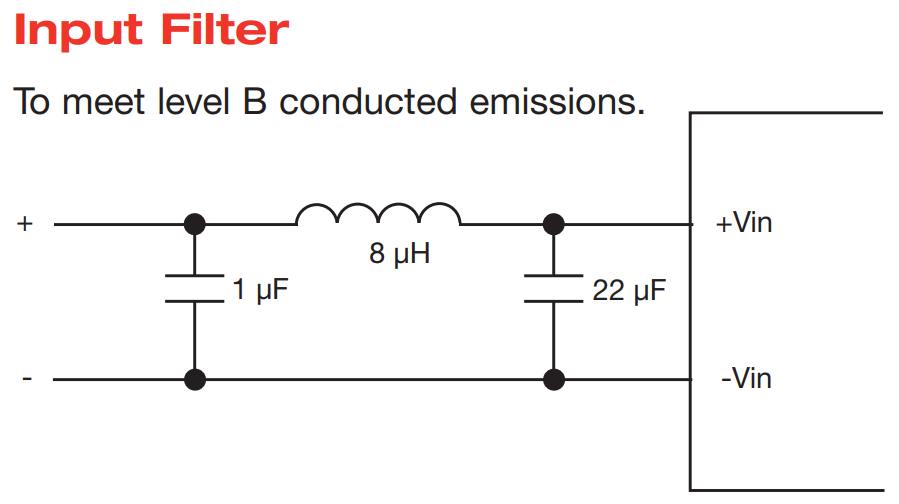
\includegraphics[scale=1.5]{content/images/emissionckt.png}
	\caption{XP Power JCA0605S05 Level B Emission Circuit \cite{isolatedvoltageconverter}}
	\label{fig:emissionckt}
\end{figure}

Applying the mentioned solutions, problems faced due to power have been dealt with and the constructed system safety is ensured.

\subsection{Mechanical Design}
In A4MCAR, the RC-Car chassis kit Tamiya TT01-E \cite{tt01e} have been used. The chassis kit consists of several parts and it is a kit that is used in professional RC-Car competitions. The Figure in \ref{fig:rccarparts} show the constructed Tamiya TT01-E chassis kit along with several other equipment that have been used in A4MCAR. Since the A4MCAR does not only have basic driving elements but also has many other equipments that are related to sensing, processing, and power, the space on the RC-Car would not be enough to hold the extra elements. Therefore, an extension to the existing chassis was needed. To solve this problem, an extension have been designed that is able to hold other elements used in the board with holders and screws. 
\begin{figure}[!ht]
	\centering
	\captionsetup{justification=centering}
	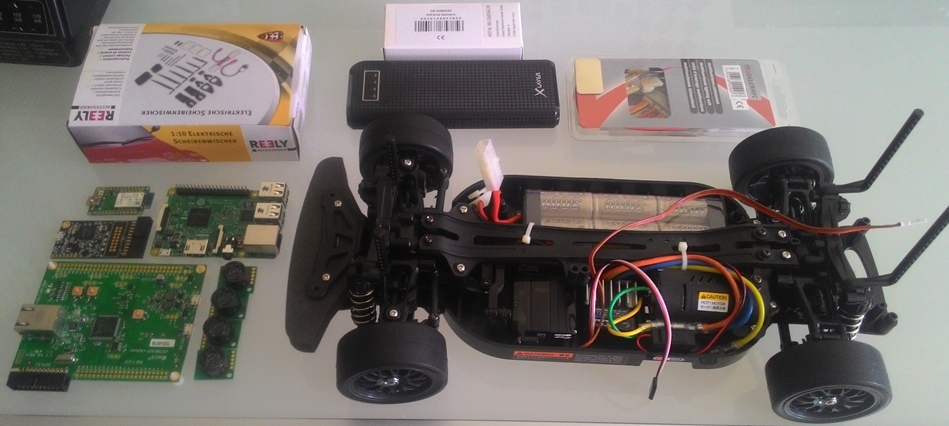
\includegraphics[width=\textwidth]{content/images/rccarparts.png}
	\caption{Tamiya TT01-E Chassis and other parts used in A4MCAR}
	\label{fig:rccarparts}
\end{figure}

An illustration of the mechanical overview that shows the designed model is shown in \ref{fig:mechanicaloverview}. This mechanical layer has been designed using a 3D model software and the software output with the .STL extension is used for the layer production using a 3D printer. Using appropriote 1mm to 2mm diameter screws, the constructed body is installed to the main chassis as an extension layer and the other elements are installed on top of this extension layer. 

\begin{figure}[!ht]
	\centering
	\captionsetup{justification=centering}
	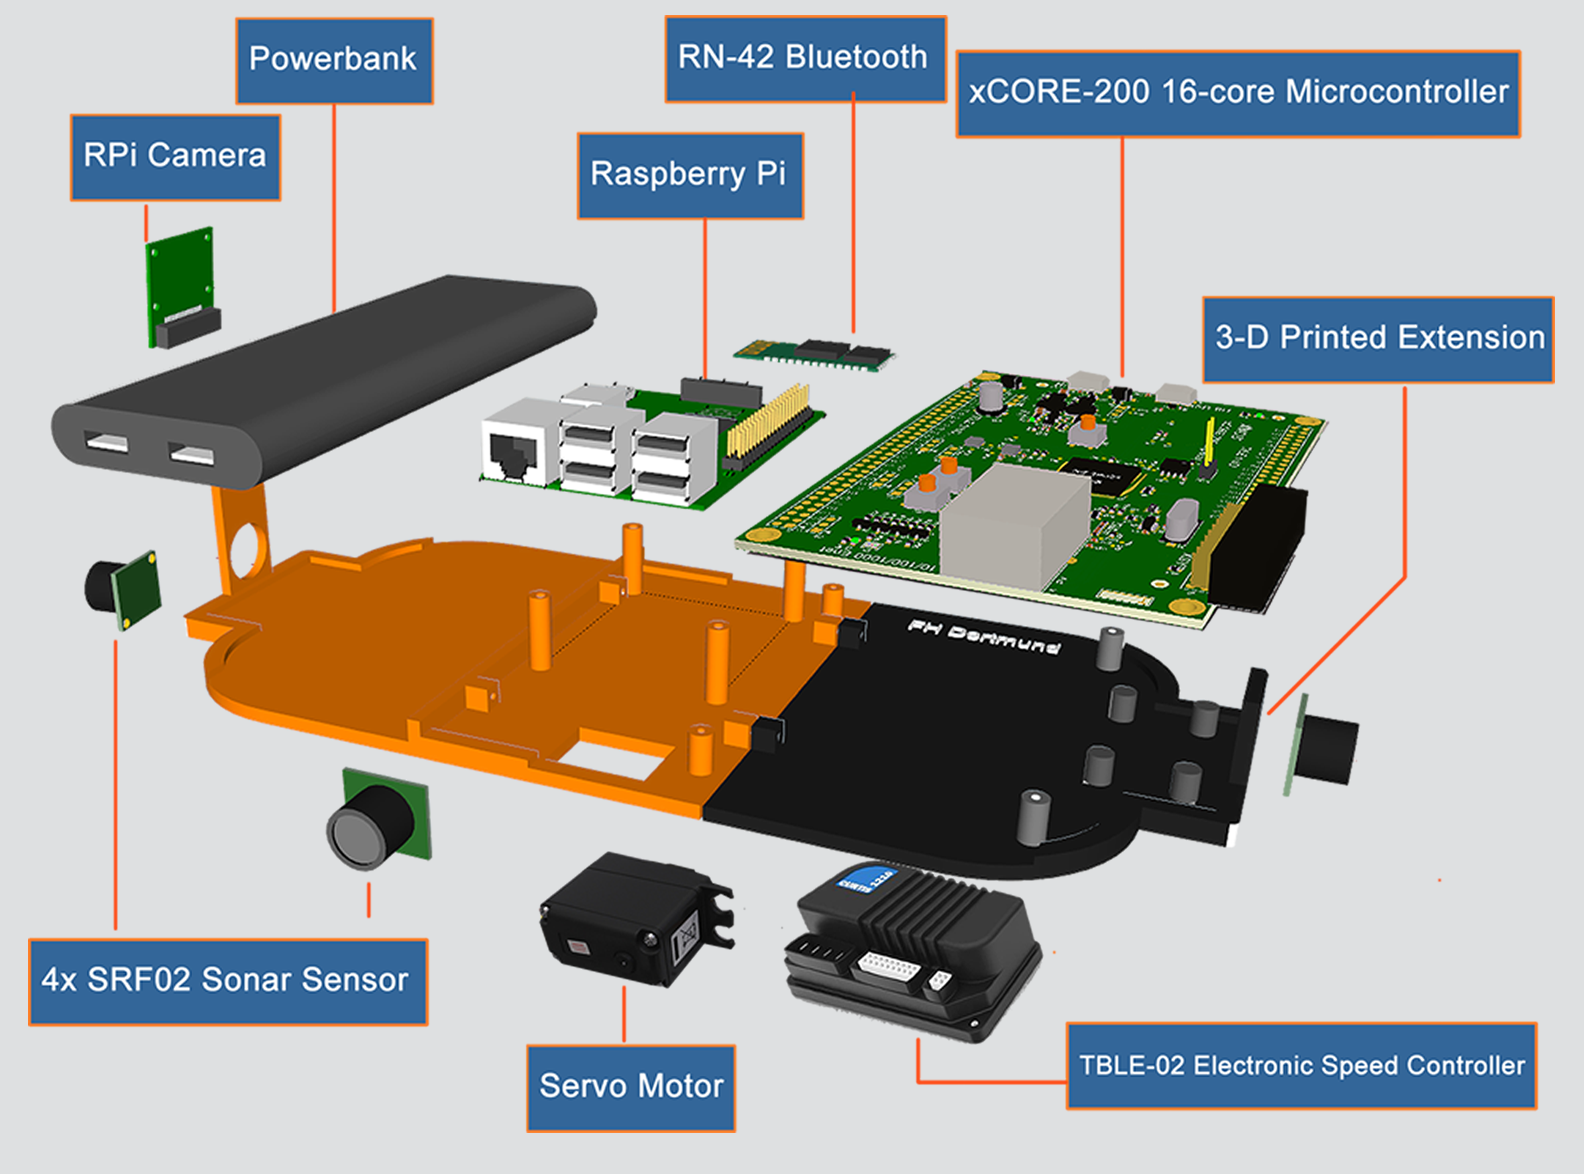
\includegraphics[scale=0.25]{content/images/mechanicaloverview.png}
	\caption{Mechanical overview of the A4MCAR}
	\label{fig:mechanicaloverview}
\end{figure}

\section{Low-Level Module Design and Implementation}
\subsection{Overview} \label{lloverviewsection}
As mentioned in the Section \ref{lowlevelmoduleinfra}, Low-level module software has been implemented on xCORE-200 eXplorerKIT using the development platform xTIMEcomposer 14.2.3. While developing with xC on xTIMEcomposer, task communication is handled by channels and interfaces. In A4MCAR, for the sake of structured development with defined variable types, interfaces are more commonly used for user-defined tasks. An software design analogy of equating provided interfaces to client interfaces in xC could be made. Similarly, required interfaces could be thought of server interfaces in xC. Using this analogy, the designed software components could be illustrated with a SysML \cite{sysml} diagram as shown in Figure \ref{fig:sysmlxmostasksbrief}.
\begin{figure}[!ht]
	\centering
	\captionsetup{justification=centering}
	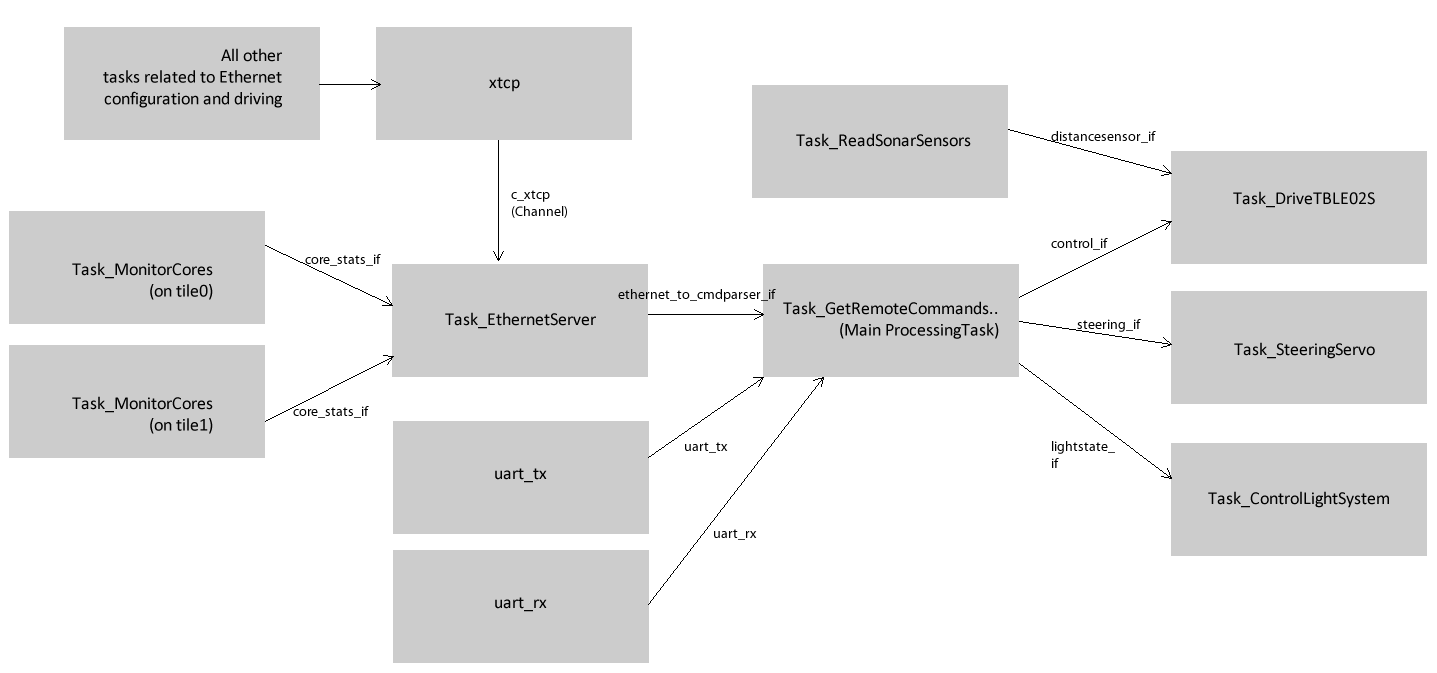
\includegraphics[width=\textwidth]{content/images/sysmlxmostasksbrief.png}
	\caption{Brief block diagram for the developed tasks and interfaces for low-level module}
	\label{fig:sysmlxmostasksbrief}
\end{figure}

The complete component diagram of the software that is developed is shown in Figure \ref{fig:sysmlxmostasks}.

\begin{figure}[!ht]
	\centering
	\captionsetup{justification=centering}
	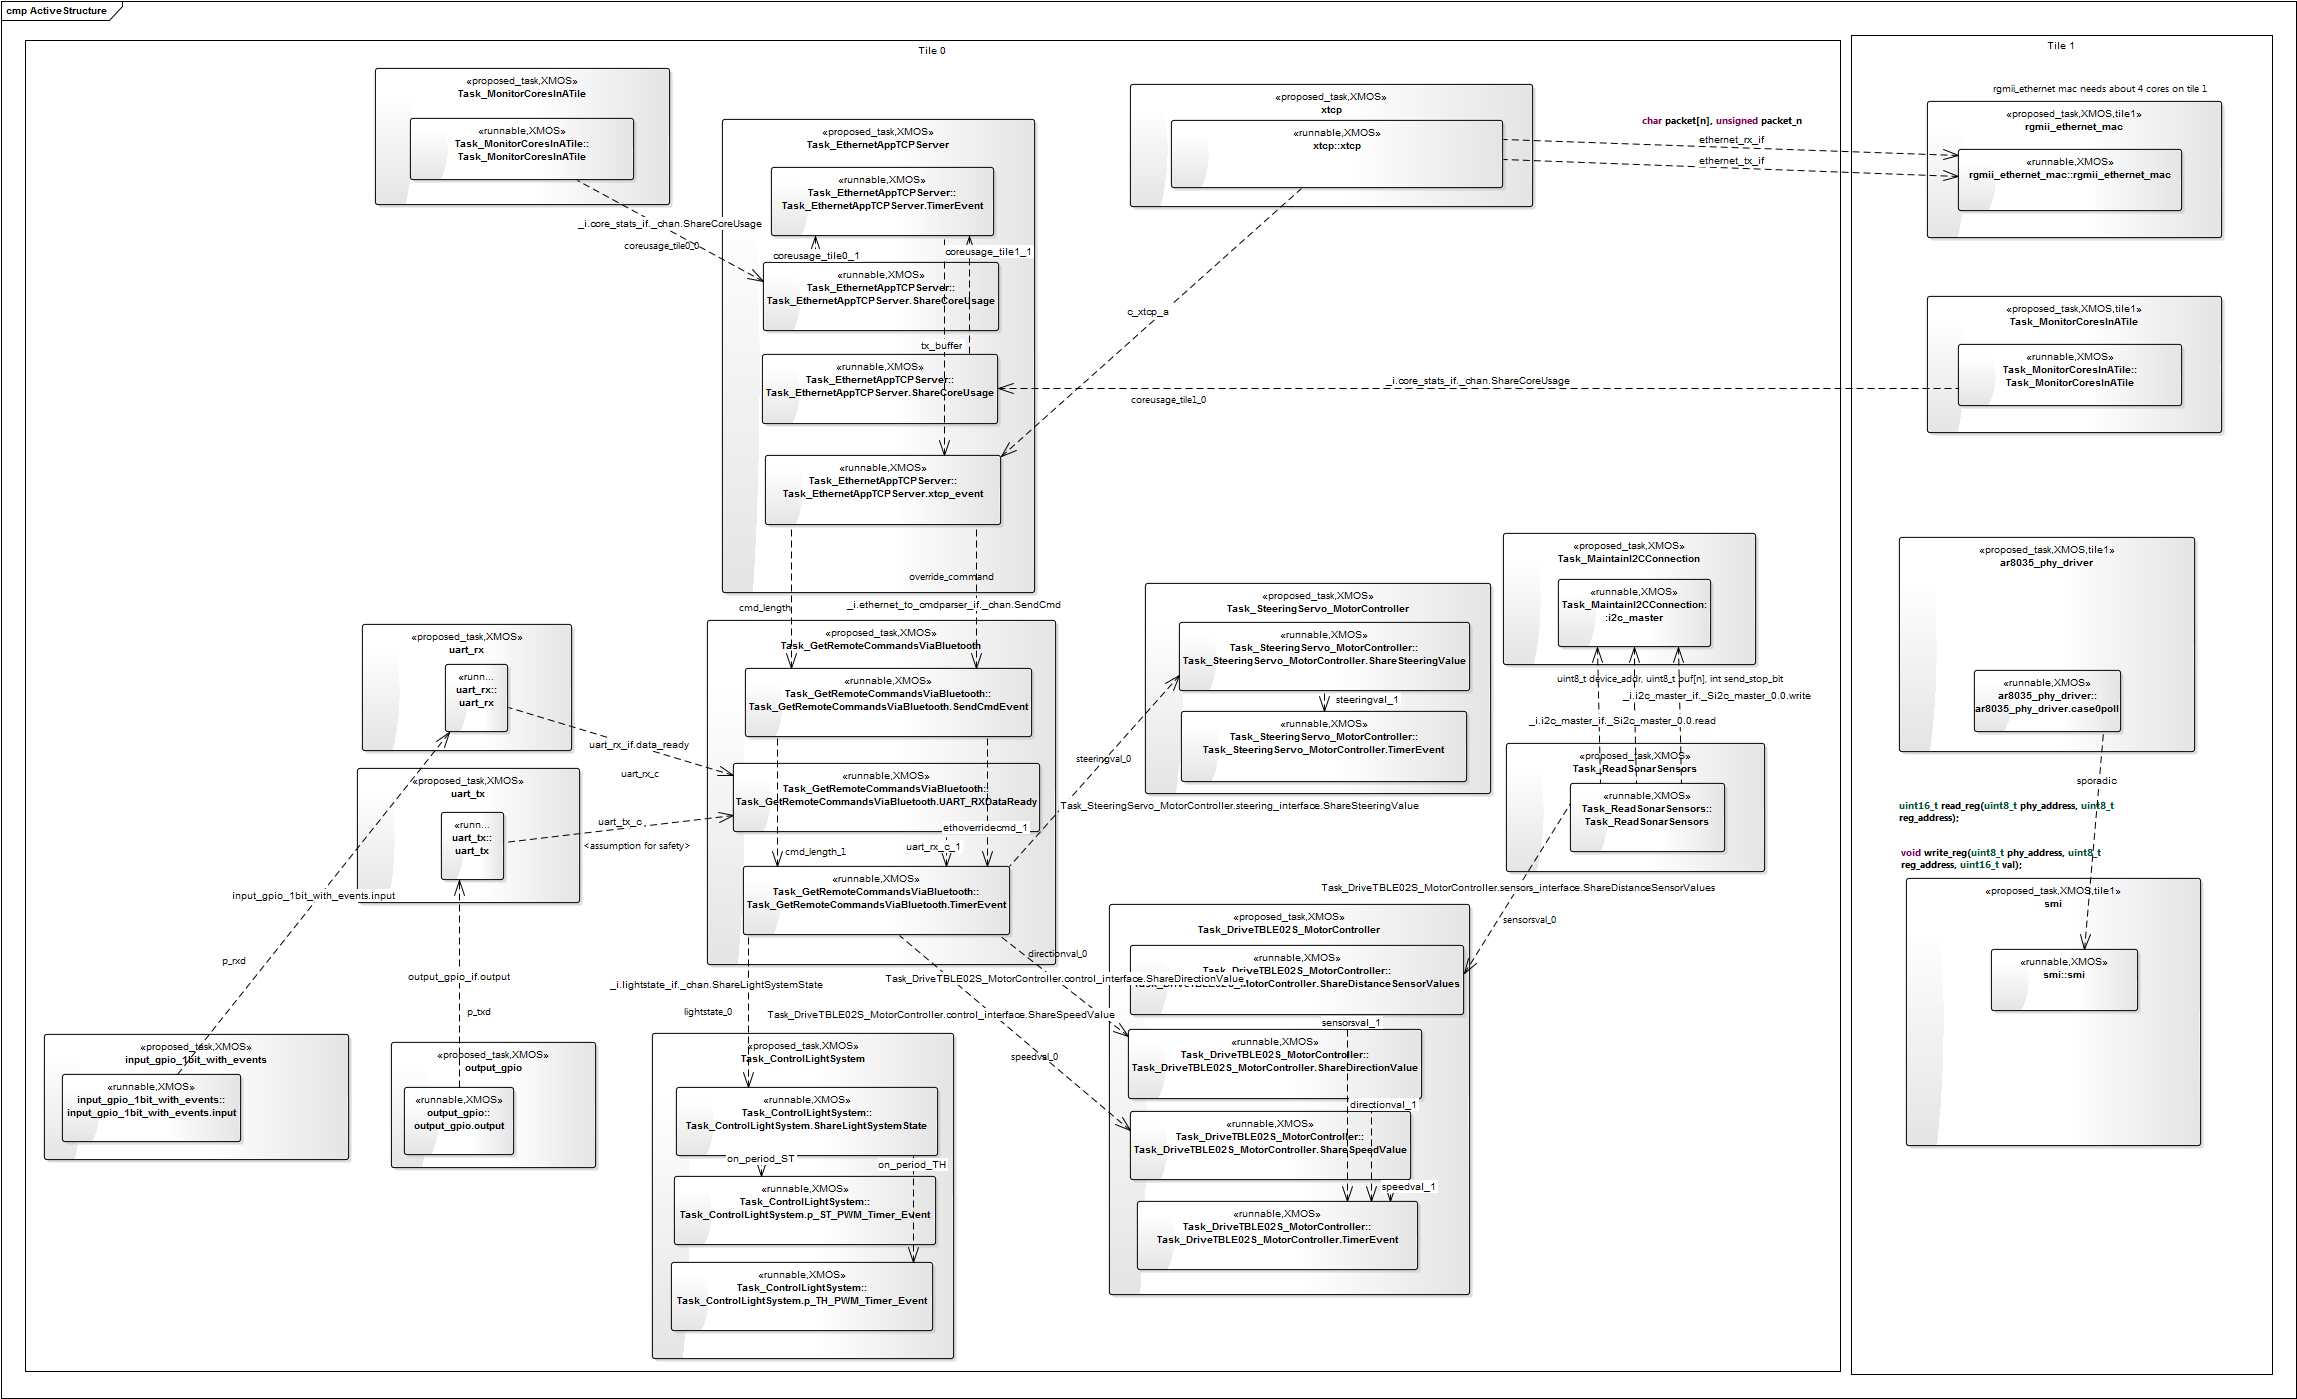
\includegraphics[scale=0.21]{content/images/sysmlxmostasks.png}
	\caption{Block diagram for the developed tasks and interfaces for low-level module}
	\label{fig:sysmlxmostasks}
\end{figure}

In xC, two essential concepts are worthy to explain in order to understand multi tasked development. First is how a task is created and the second is how tasks are connected. A task in xC is nothing but a function that has client and server ports with interfaces. Once all functions are connected using globally instantiated interface variables they start acting as tasks. An example of how a task function is declared and how functions are placed on cores and interconnected which is also some of what is implemented for A4MCAR are shown in Listing \ref{lst_exampletaskxc} and Listing \ref{lst_howtasksconnectxc}, respectively.

\lstinputlisting[caption=An Example Task Decleration in xC, label=lst_exampletaskxc, style=xc]{content/listings/lst_exampletaskxc.txt}

In the code given with the Listing \ref{lst_exampletaskxc}, it is seen that the function prototype has several arguments as client and server interfaces. Those interfaces indicate the role of the data communication using the respective interface. When a task function takes client interface as an argument, it means that the task function sends data to that interface, whereas when a task function receives a message using event handles it is given by the server keyword.

\lstinputlisting[caption=An Example of How Tasks are Placed and Interconnected in xC, label=lst_howtasksconnectxc, style=xc]{content/listings/lst_howtasksconnectxc.txt}

The Listing in \ref{lst_howtasksconnectxc} shows in which tile and at which core a task will be places. Using the par keyword (given in Line 1), every line of code in that particular code block will be paralellized using the scheduler of xCORE. 

All the source and header files that contain task functions and that are developed in this fashion are shown in Figure \ref{fig:fullfiletree}.
\begin{figure}[!ht]
	\centering
	\captionsetup{justification=centering}
	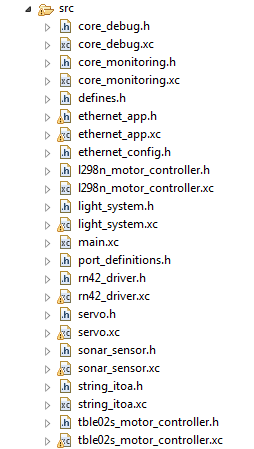
\includegraphics[scale=0.8]{content/images/fullfiletree.png}
	\caption{Full file tree for all the tasks developed for low-level module}
	\label{fig:fullfiletree}
\end{figure}

\subsection{Actuation}
\subsubsection{Acceleration} \label{accelerationsection}
For acceleration and deceleration, a brushless DC motor is controlled by delivering PWM signals to the TBLE02-S Electronic Speed Controller. The task and how it is connected to other tasks can be seen in Figure \ref{fig:sysmlxmostasksbrief}. In order to deliver the desired PWM signal, a task that use timers have been created which is given in Listing \ref{lst_tble02task}. The created template of the task in Listing \ref{lst_tble02task} is not only used for the acceleration task, but also used for the other tasks that use PWM signaling to control other devices. In the task, it is seen that in order to generate the desired duty cycle, the amount of time for which the output signal must be on and off are calculated (Lines 19 through 38) and the output port is toggled (Lines 39 through 48) accordingly. The port toggling is done inside a timer event (shown in Line 17) that is dynamically delayed given the calculated on and off times.

\newpage\lstinputlisting[caption=Created PWM signaling template, label=lst_tble02task, style=xc]{content/listings/lst_tble02task.txt}
The desired PWM pulse widths are taken from the TBLE02-S Electronic Speed Controller manual and the overall PWM period has been set to 20ms which is the standard period for most of the controllers. Since the motor speed is very high and it is not desired in our application, the pulse widths are manipulated in order to reach lower speeds in full force. The interface 'control\texttt{\_}if' (Line 9 and Line 13) is used that delivers a number between 0-100 in order to express speeding information while also delivering a direction value which is either FORWARD (0) or REVERSE (1). With this information, the developed task is able to control the acceleration of the A4MCAR. Additionaly, the acceleration task is modified in order to control acceleration using proximity sensor inputs for safety. Minimum safest front distance is set to 50 centimeters.

Acceleration task and how it data is transferred between other tasks can be seen in the software component diagram in Figure \ref{fig:sysmlxmostasksbrief} with acceleration task having the function name 'Task\texttt{\_}DriveTBLE02E'.

\subsubsection{Steering}
Steering of the A4MCAR is done with the help of a Servo motor that is also controlled with PWM signaling. As mentioned in the Section \ref{accelerationsection}, the tasks that are related to PWM use the template from Listing \ref{lst_tble02task}. For steering the interface 'steering\texttt{\_}if' is used which is set to 0 for very left and 100 for very right positions. Additionally, the two changes that are made to the acceleration task (from Listing \ref{lst_tble02task}) could be listed as follows:
\begin{itemize}
	\item The pulse widths are altered in order to conform a servo motor's behavior which is usually 1.5ms pulse for stationary position, 1-1.5ms for left steering and 1.5-2.0ms for right steering. For A4MCAR, these values are set to 1.3-1.5ms for left steering and 1.5-1.75ms for right steering in order to get rid of the issue of servo motor turning more than its holding platform could handle and damaging its gears.
	\item On and off periods are calculated differently as compared to what is shown in the Listing \ref{lst_tble02task}. The Listing in \ref{lst_servotask} shows the calculation of the periods using the pulse width values.
	\lstinputlisting[caption=Calculation of on and off times for servo control, label=lst_servotask, style=xc]{content/listings/lst_servotask.txt}
\end{itemize}

Steering task and how it data is transferred between other tasks can be seen in the software component diagram in Figure \ref{fig:sysmlxmostasksbrief} with steering task having the function name 'Task\texttt{\_}SteeringServo'.

\subsubsection{Braking}
Since the motor that is used in A4MCAR is a brushed motor, it does not come with braking features. Therefore, a braking mechanism was needed to be implemented. For this purpose, a 2-channel relay board from Sainsmart (shown in Figure \ref{fig:relayboard}) has been used to short circuit the terminals of the motor when braking is required. In the Figure \ref{fig:brake}, the circuit portion that is controlling the operation of the brake is given.
%brushless motor needed, three connections (Orange connection), and mode setup. (source: tble02s manual)
\begin{figure}[!ht]
	\centering
	\captionsetup{justification=centering}
	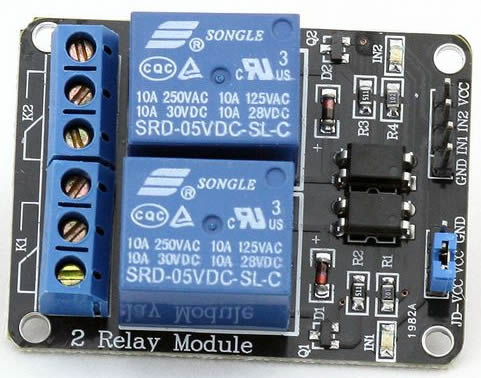
\includegraphics[scale=0.4]{content/images/relayboard.jpg}
	\caption{Two-channel relay board that is used for braking}
	\label{fig:relayboard}
\end{figure}

\begin{figure}[!ht]
	\centering
	\captionsetup{justification=centering}
	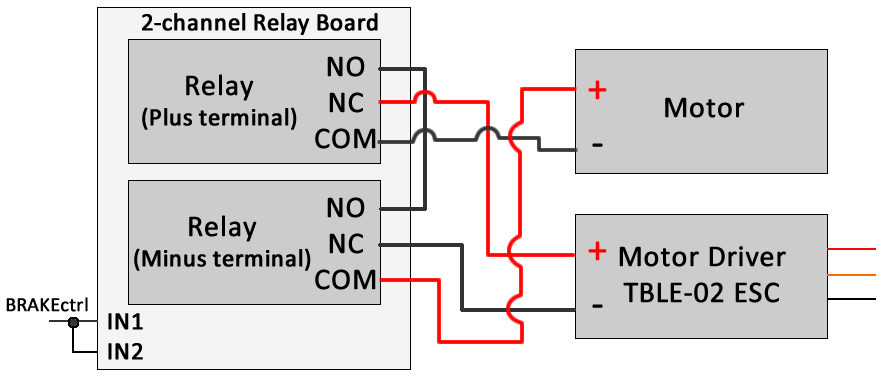
\includegraphics[scale=0.5]{content/images/brake.png}
	\caption{Relay circuit to control braking}
	\label{fig:brake}
\end{figure}

Normally, the terminals of the motor and the motor driver (Electronic Speed Controller TBLE-02) are connected together. Using the switching mechanism that is provided by the relays, motor terminals are short circuited when the relays are activated. 

Relays have three essential input or output signals that are used in operation. Those signals involve IN, NO, NC, and COM. With simple switching in mind, the operation of the relay can be described. When IN signal is low, COM is short circuited with NO whereas when IN signal is high, COM signal is short circuited to NC signal. 

By using this mechanism and using the COM signal output, motor is supplied by motor driver normally and motor terminals are short circuited when the braking is required. The control has been done by giving the same input to IN1 and IN2 signals, IN signals for each relay, from the xCORE-200 eXplorerKIT. The integration of the braking mechanism to the system is done at the acceleration task, in which when the received speed is zero, brake is activated. Since the relay works with only 5V input signal for the IN terminal, BRAKEctrl signal, given in Figure \ref{fig:brake} is connected to the xCORE-200 eXplorerKIT through a 5V to 3.3V converter, which is also shown in the schematics given in the Figure \ref{fig:RCCAR_Schematics}.

\subsection{Proximity Sensing}
As stated in the Section \ref{lloverviewsection}, the proximity sensing is handled via four SRF-02 ultrasonic sensors connected to an I\textsuperscript{2}C network. In the software, 'lib\texttt{\_}i2c' from XMOS is used in order to handle communication with the peripheral. 

The pseudo version of the proximity sensing task is given in Listing \ref{lst_proximitysensing}. The proximity sensing task is a periodic task that polls individual ultrasonic sensors using their respective addresses (Line 12 and Line 13) in order to obtain what is the distance perceived by front, rear, left, and right sensors. In order to handle this in a modular manner, device addresses are placed in the header file. Furthermore, the task that maintains I\textsuperscript{2}C communication alongside proximity sensing task is seperated and the two tasks are connected using 'i2c\texttt{\_}master\texttt{\_}if' interface (shown in Line 1). The sensing is achieved every 0.2 seconds within a timer event (shown in Line 7) and when the sensing of each sensor complete, the value is sent by its respective interface 'distancesensor\texttt{\_}if' to the acceleration task (Line 22). 

Proximity sensing task and how it data is transferred between other tasks can be seen in the software component diagram in Figure \ref{fig:sysmlxmostasksbrief} with proximity sensing task having the function name 'Task\texttt{\_}ReadSonarSensors'.

\lstinputlisting[caption=Proximity sensing task, label=lst_proximitysensing, style=xc]{content/listings/lst_proximitysensing.txt}

\subsection{Lighting System}
The light system of the A4MCAR is a light module from the RC-Car parts producer Modelcraft that is driven with PWM. The module uses two PWM channels: one for light adjustment due to steering input, one for light adjustment due to acceleration input. Similarly to all the other PWM control tasks, PWM signal generator template that is given in \ref{lst_tble02task} has been used in order to generate correct pulse widths for the light system. The task that is given in \ref{lst_tble02task} has been adjusted to have two timer events for each PWM channel as opposed to one timer event. Desired pulse widths for several modes are contained in the header file of the light system task and these modes have been selected given the steering, angle, and gear inputs from the Bluetooth communication task. The functions regarding pulse width time generation for different light system modes have also been created. 

Light system task and how it data is transferred between other tasks can be seen in the software component diagram in Figure \ref{fig:sysmlxmostasksbrief} with light system task having the function name 'Task\texttt{\_}ControlLightSystem'.

\subsection{Bluetooth Communication}
In order to configure RN42 Bluetooth module \cite{rn42datasheet} as slave to communicate with the Android phone and receive data, UART communication have been implemented using 'lib\texttt{\_}uart' from XMOS. In order for the UART communication to be handled correctly, CTS and RTS pins of the RN42 module should be short circuited since a data flow protocol such as RS232 is not being used in our application. UART library has been configured to have a buffer size of 512 bytes and baudrate of 115200bps which is a high speed UART data rate standard that conforms many microcontrollers. Several tasks have been implemented such as uart\texttt{\_}rx, uart\texttt{\_}tx, and the Bluetooth communication task in order to implement bluetooth control feature into the A4MCAR. While uart\texttt{\_}rx and uart\texttt{\_}tx tasks handle port access and data transfer in respective directions using sporadic events, the Bluetooth communication task is responsible for configuring the Bluetooth module and receiving driving commands. For an easy communication, a string with a number of bytes is constructed and interpreted by the Bluetooth communication task. This string which we refer to as 'driving command' is given and explained in the Figure \ref{fig:bluetoothcommand}. 
\begin{figure}[!ht]
	\centering
	\captionsetup{justification=centering}
	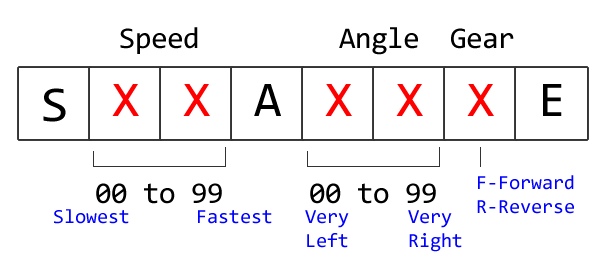
\includegraphics[scale=0.6]{content/images/bluetoothcommand.png}
	\caption{Driving command format generated to contain speed, angle, and gear information}
	\label{fig:bluetoothcommand}
\end{figure}
The command parsing and how the received data is accumulated to other tasks is given in the Listing \ref{lst_bluetoothtask}. 

The operation of this portion of the task could be explained as follows:
\begin{itemize}
	\item A preprocessor macro has been defined which is RN42\texttt{\_}INITIAL\texttt{\_}CONFIG. This macro activates the configuration function which configures RN42 module with slave mode. This configuration is shown in the Line 2 of the Listing \ref{lst_bluetoothtask}. It should be noted that the configuration should only be done once per bluetooth module.
	\item Receiving driving command using uart receive event (Line 7), integrity check for the command (Line 20), and parsing in order to obtain speed, angle, and gear values (Line 21) has been implemented.
	\item Since driving command is not the only source of actuation data source for A4MCAR and it could have overriding commands over Ethernet from high-level module image processing task, ethernet override is handled with an integrated event in the Bluetooth communication task (shown in Line 11).
	\item Reverse driving mode is not entered by the TBLE02-S Electronic Speed Controller unless the motor fully stops. To achieve this, normally user has to select reverse mode several times from the controller. In order to get rid of this issue, once the reverse command is received, software enters reverse mode a few times with very short delays, thus users can select it only once and enjoy driving without having to select the mode a few times by themselves. This implementation is shown in Line 23 in the Listing \ref{lst_bluetoothtask}.
	\item The obtained control and steering values are sent to the associated task functions in order to handle the actuation (Lines 27 through 29).
\end{itemize}
\lstinputlisting[caption=Bluetooth communication task pseudocode, label=lst_bluetoothtask, style=xc]{content/listings/lst_bluetoothtask.txt}

Bluetooth communication task and how it data is transferred between other tasks can be seen in the software component diagram in Figure \ref{fig:sysmlxmostasksbrief} with bluetooth communication task having the function name 'Task\texttt{\_}MainProcessingAndBluetoothControl'.

\subsection{Ethernet (TCP) Server Implementation} \label{llethsection}
TCP server of the A4MCAR low-level module acts as the only source of communication that is implemented between low-level module and high-level module. The TCP communication that is implemented for this basic data transmission and reception could be called as Telnet \cite{telnet}. As mentioned, while overriding driving command (Figure \ref{fig:bluetoothcommand}) is sent from high-level module (configured as the Telnet server) to low-level module (configured as the Telnet client), for the visualization purposes the core utilization information is sent from low-level module to high-level module. On the low-level side, library that is provided from XMOS 'lib\texttt{\_}xtcp' is used with the following adjustments:
\begin{itemize}
	\item The application notes from XMOS involves only UDP applications. This application has been manipulated in order to have TCP protocol based Telnet server
	\item The TCP server has been configured with a static IP address and with a bind port.
	\item Data receiving and transmitting event handlers as well as the interface that sends the driving command to the Bluetooth communication task have been created.
	\item Since the media-independent interface (MII) of xCORE-200 eXplorerKIT supports up to 1000Mbps reduced gigabit media-independent interface (RGMII), the ethernet server task takes up to 3 to 4 cores in order to be parallelized. In order to reduce the excessive core usage, this interface have been reduced to a speed of 100Mbps by the software that takes about 2 cores in order to be parallelized efficiently. Furthermore, it is important to mention that since application in the A4MCAR does not require a gigabit ethernet connection, this decrease in the speed did not affect the performance of the communication.
\end{itemize}

TCP server task and how it data is transferred between other tasks can be seen in the software component diagram in Figure \ref{fig:sysmlxmostasksbrief} with TCP server task having the function name 'Task\texttt{\_}EthernetServer'.

\subsection{Core and Tile Monitoring}\label{coremonitoringsection}
Core monitoring task that is responsible for finding core utilization percentage and sending it to the TCP server task is created for the two individual tiles of the xCORE-200 eXplorerKIT. By checking the status register 'XS1\texttt{\_}PSWITCH\texttt{\_}T0\texttt{\_}SR\texttt{\_}NUM' that is mentioned in the XMOS datasheet \cite{xmosdatasheet}, and polling this register with a maximum polling rate of 1250Hz, whether a core is busy or idle at a given time is detected. A code snippet that is responsible for this operation is given in Listing \ref{lst_coremonitoring}. 

\lstinputlisting[caption=Finding busy and idle cycles in XS1 architecture, label=lst_coremonitoring, style=xc]{content/listings/lst_coremonitoring.txt}

In the given listing, the status register 'XS1\texttt{\_}PSWITCH\texttt{\_}T0\texttt{\_}SR\texttt{\_}NUM' and the processor state has been read (Line 5 and Line 9, respectively) for every core in order to find which core is idle and which core is busy at that moment. 

The obtained busy and idle cycles are then converted to a percentage value with the following Equation:
\begin{equation}
core\texttt{\_}usage\texttt{\_}percentage=\frac{busy\texttt{\_}cycles}{busy\texttt{\_}cycles + idle\texttt{\_}cycles} 100
\end{equation}
Further features introduced in core monitoring task could be listed as follows:
\begin{itemize}
	\item An interface is created, that is 'core\texttt{\_}stats\texttt{\_}if' in Figure \ref{fig:sysmlxmostasksbrief}, in order to send core utilization percentage to the TCP server task. 
	\item A preprocessor macro FLOATING\texttt{\_}POINT\texttt{\_}SHOW is also created in order to find core utilization percentage in floating point format for better precision if desired.
\end{itemize}

Observing the results have showed that the user created applications for the low-level module in A4MCAR are not very time intensive and that is why some of the tasks resulted in a core utilization value that is lower than 0 percent.

Core monitoring tasks and how their data is transferred between other tasks can be seen in the software component diagram in Figure \ref{fig:sysmlxmostasksbrief} with tasks having the function names 'Task\texttt{\_}MonitorCores'.

\section{High-Level Module Design and Implementation}
\subsection{Overview}
High-level module of the A4MCAR is composed of several processes and threads running under Raspbian \cite{raspbiandownload} distribution of Linux Operating System that is designed for Raspberry Pi 3. In the Section \ref{hlinfrasection}, the operation of Linux kernel is briefly introduced. During the compilation, debugging and execution of the developed processes, several development platforms such as Python 2.7 shell \cite{python27}, GNU C Compiler (GCC) \cite{gcc} have been used. Although it should be noted that remote development using Eclipse IDE \cite{remotedebuggingeclipse} is also possible, the development of A4MCAR has been done using the aforementioned development platforms by connecting into the Raspberry Pi 3 using SSH connection. While the main processes involve C, C++, Python, and Bash \cite{bash} languages, via the capability of the integrated web server to serve web pages, several other scripting and markup languages such as HTML, CSS, JavaScript (with AJAX \cite{howajaxworks} and jQuery \cite{jquery} frameworks) have also been used. The operation of the user developed processes along with third party utility processes and threads that are integrated into the system are given in the Figure \ref{fig:rpicomponents}. 
\begin{figure}[!ht]
	\centering
	\captionsetup{justification=centering}
	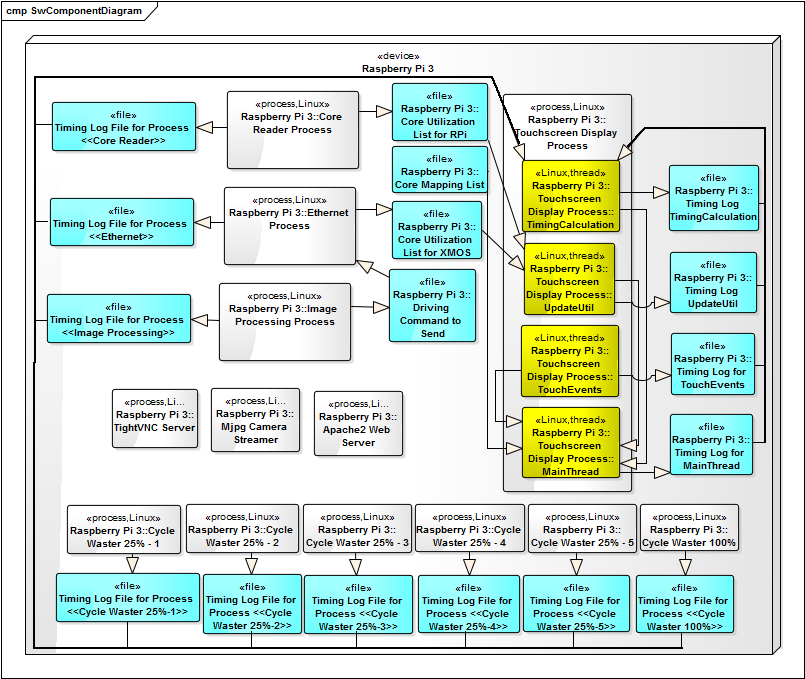
\includegraphics[width=\textwidth]{content/images/rpicomponents.png}
	\caption{High-level module software component diagram including files and file accesses}
	\label{fig:rpicomponents}
\end{figure}

Since cross development platforms using languages such as C, C++ and Python have been used in A4MCAR high-level module, the multi-tasking is handled in mostly the process layer rather than in thread or task level. That means that each process are executables of their own using different libraries and compilers. However, the touchscreen display process is designed with several threads.

In the Figure \ref{fig:rpicomponents}, it is also seen that the communication between user developed processes are handled with mostly file accesses. All file accesses are asynchronous and there is no event to wait for data or require data within some time as it is low-level module inter-process communication. This should indicate that the communication using read-write accesses does not constrain the processes as it is in a regular inter-process communication. Furthermore, it should be noticed from the Figure in \ref{fig:rpicomponents} that although a process is able to read from many files, there is no example of two or more processes trying to write to the same file. Reading from many files is not critical, while the latter (i.e. two or more processes trying to write to the same file) should be handled by cross-process mutexes or semaphores that would be able to lock and unlock the same physical memory space from cross-processes. Although not valid in our case, it should be known that by using the existing cross-process mutexes or creating a semaphore mechanism, one should be able to allow two or more processes to write to the same file \cite{linuxkernelbook}. However, it can be commented that the locking of the files are handled with the locks from OS kernel in our case and there is no need to create new locks in the applications for file accesses.

The way multi-tasking is handled with this constructed software architecture (in the Figure \ref{fig:rpicomponents}) is that every process is run by an external script at the boot time (or via touchscreen interface, which is the main control interface in our case) and their scheduling is handled by the Linux kernel. While the scheduling is not manipulated, the mapping or pinning of processes to different cores and evaluating them are the focus of A4MCAR in order to find the most optimal parallelization solution.

Regarding hardware, the high-level module is connected to two devices. The interfacing of these devices, a Raspberry Pi camera v2.0 and a Touchscreen display is illustrated in the Figure \ref{fig:hwoverview}. It is seen in the figure that interfaces such as HDMI, SPI, and CSI have been utilized. In the following sections, hardware communication and the related software will be further explained.
%%Full names as appendix  ??? MAYBE LATER
\subsection{Implemented Online Timing Features and Making Processes Schedulable} \label{onlinetiming}
In order to seek an assessment technique to compare timing performance of different distributions and ensure that the developed processes and threads are schedulable, online timing features are implemented in the user-developed processes of the high-level module of A4MCAR. Thus, while applications are running, a performance evaluation could be done with the help of the those features. The code skeleton is developed for both Python and C,C++ applications and the applications are integrated on top of the skeleton with timing features. Therefore, it is important to understand how each application that will be discussed in the following sections are timed.

Recall that in the Section \ref{schedulingsection} the timing properties in a scheduled system is explained that is shown in Figure \ref{fig:scheduling}. By making use of the figure, limitations of implementations and the implemented timing features could be listed as follows:
\begin{itemize}
	\item Because the values such as IPT, CETs and RT (referred from the Figure \ref{fig:scheduling}) are out of our reach since they are hidden in the Linux kernel, in the online timing analysis features that are implemented, the aforementioned values have been neglected. With offline scheduling analysis, however, CET values could be easily obtained.
	\item Recording the the start and end times of execution using an accurate clock. For that purpose, in computers there are two types of clocks: (1)- User CPU clock and (2)- System CPU clock. While user CPU clock is used for finding out how long it has passed since the program has started, the system CPU clock takes place in the kernel space and measures how long it has passed since 1st of January, 1970. The latter clock was found as the viable solution as user CPU clock would not allow comparison along the entire Linux kernel. In the code, functions time.time() for Python and clock\texttt{\_}t clock() have been used in order to record start and end times more accurately \cite{cpuandusertimes} \cite{cpuandusertimes2}.
	\item Finding the execution time (ET) of one iteration using the following Equation, provided that start\texttt{\_}time is the time recorded before the iteration and end\texttt{\_}time is the time recorded after the iteration. The units are all seconds.
	\begin{equation}
	execution\texttt{\_}time=end\texttt{\_}time - start\texttt{\_}time
	\end{equation}
	In the version that is developed for C language, since clock\texttt{\_}t is able to measure clock cycles rather than seconds, the Equation is changed to the following:
	\begin{equation}
	execution\texttt{\_}time=\frac{end\texttt{\_}time - start\texttt{\_}time} {CLOCKS\texttt{\_}PER\texttt{\_}SEC}
	\end{equation}
	
	\item Finding the slack time (ST) is one of the most important tasks that is within the scope of the online timing features because as a rule of thumb, we could assess the timing performance by saying that if a process has a higher slack time than before, it means that that task is better utilized compared to before as the idle time the CPU is doing some other task is more than what it used to be. The slack time of a previous iteration is measured by the following Equation, provided that the calculation takes place right after start time is recorded and IPT is neglected. It should also be noted that the C language version could be created by dividing the clock cycles with the clock cycles per second (CLOCKS\texttt{\_}PER\texttt{\_}SEC) in the same manner as execution time.
	\begin{equation}
	previous\texttt{\_}slack\texttt{\_}time=start\texttt{\_}time - end\texttt{\_}time
	\end{equation}
	
	\item In order to keep a constant period while the process is being scheduled, the processes are delayed dynamically between each iteration. Thus, processes which have a constant period could be modeled easier and having the constant period will make the process or thread schedulable. In order to achieve a constant period each process are delayed by the following:
	\begin{equation}
	delay\texttt{\_}time=period - execution\texttt{\_}time
	\end{equation}
	However, if the execution time of a process is bigger than its period, that process could be counted a process that missed its deadline, given that its period is equal to its deadline due to practicality. In addition, it should be known that the deadline miss percentage is another important criteria in order to assess parallelization quality as it is normally undesired to have missed deadlines. In case of a missed deadline in A4MCAR, the process is not delayed.
	
	\item As seen in \ref{fig:rpicomponents}, there are many timing log files that are created. Those timing log files are created within every user-defined process and later are used in the Touchscreen Display application.
\end{itemize}

While each processes and thread are constructed in the manner that is explained, the overall online evaluation is handled within the Touchscreen Display process in the TimingCalculation thread (shown in Figure \ref{fig:rpicomponents}),  In Chapter \ref{informationchapter}, the details about these will be given.

An example of the timing skeleton for Python-running processes are given in the Listing \ref{lst_timingskeleton}. The user-defined Python-running applications have been created using this template, and the space that is left for task content is used for the actual features of that task.

\lstinputlisting[caption=Online timing features implemented in Python language, label=lst_timingskeleton, style=python]{content/listings/lst_timingskeleton.txt}

In the given code by the Listing \ref{lst_timingskeleton}, following remarks should be made:

\begin{itemize}
	\item Lines 2 through 5 indicate which libraries are used.
	\item Between the Lines 8 and 13, global variables to hold the time values are initialized.
	\item A timing data logging function is created (Lines 15 through 33). In this function, timing log file is opened (Lines 23 through 26), execution time is calculated after end time is recorded (Line 27 and Line 28) and then all the timing values at that instant is written into the opened text file (Lines 29 through 33). After the write operation the file is closed (Line 33).
	\item In the loop section of the process start time and previous slack time are recorded (Lines 37 through 38) before the actual task content (Lines 40 through 42) is executed. After the task content is executed, timing log is created by using the timing data logging function (Line 45) and then the task is delayed according to its period by finding the delay\texttt{\_}time that was given in (4.5). This delay operation is also given in the Listing \ref{lst_timingskeleton} at the Lines 48 through 49.  
\end{itemize}

\subsection{Core Reader}
To help with the utilization assessment and visualization purposes, a core reading process is developed that monitors cores every three seconds and writes the core usage information to a text file. For that purpose, the 'psutil' module \cite{psutil} from Python is used. The 'psutil' module allows to find information of Linux processes and cores. The core usage information for four cores of Raspberry Pi that is logged into a text file is then used for visualization in the web interface and the touchscreen interface. 

With the help of a simple function the core usage information is easily retrieved. The function is given in the Listing \ref{lst_psutil}. It should be noted that 'd' in the listing is an array with 4 elements, each of which indicating core usage for individual cores.

\lstinputlisting[caption=Psutil function to retrieve core utilization information , label=lst_psutil, style=python]{content/listings/lst_psutil.txt}

\subsection{Ethernet (TCP) Client Implementation}
In the Section \ref{llethsection}, TCP server implementation using the xCORE-200 eXplorerKIT has been discussed. In order to maintain a sound data communication between low-level module and high-level module, a TCP client process is implemented in the high-level module. Since Python language offers very stable and easy-to-use threading support and exception handling, the TCP client implementation is done using Python. The 'socket' library \cite{socketpython} in Python is capable of delivering several functions and objects that are used for this purpose. The TCP client has been configured to have non-blocking data reception with 0.5 second period and with a timeout of 2 seconds. While the data reception is handled by an additional thread, operations such as connecting to the server, binding to the server port, and sending data periodically is handled in the main thread. The overriding driving command which is send to the low-level module is read from file before data transmission. It should be also noted that after the data reception the content is written to the file which is responsible for holding low-level module core usage information. This communication between high-level module and low-level module is illustrated in the deployment diagram given by the Figure \ref{fig:ethernetdeployment}.

\begin{figure}[!ht]
	\centering
	\captionsetup{justification=centering}
	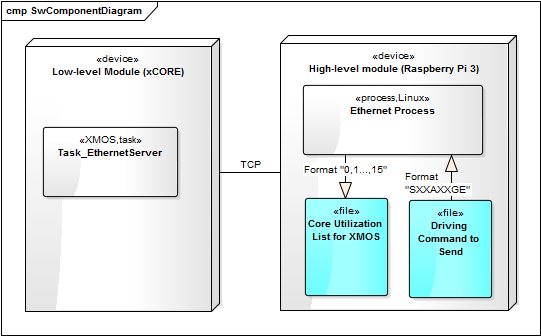
\includegraphics[scale=0.7]{content/images/ethernetdeployment.png}
	\caption{Deployment diagram showing Ethernet communication}
	\label{fig:ethernetdeployment}
\end{figure}

\subsection{Web Server and its Applications}
\subsubsection{Web Server}
In order to develop a web interface for the A4MCAR, a web server is installed and configured to the high-level module. Web servers are responsible for processing HTTP requests and delivering HTTP responses \cite{apacheguide}. The HTTP requests and responses are usually visualized using a web browser from clients in the form of web pages \cite{apacheguide}. In A4MCAR high-level module, Apache 2 web server is installed and configured as the web server since it is an open-source, robust, light-weight cross-platform that has a large user community. Additionally, another reason Apache 2 is selected is that it is capable of serving for script languages such as PHP and Python, which are used in A4MCAR applications.

Just like a Telnet server, a web server is bind to a port in a wireless or wired network. Although for different communication channels one could use different ports, web servers usually use the port number 80. Another difference of a web server is that unlike a telnet server, the data that is sent and interpreted is in the HTTP (HyperText Transfer Protocol) \cite{webserver} format unlike the TCP (Transmission Control Protocol) format. How web servers and web browsers work in order to help us visualize web pages is illustrated with the Figure \ref{fig:webserver} \cite{webserver}. \\

\begin{figure}[!ht]
	\centering
	\captionsetup{justification=centering}
	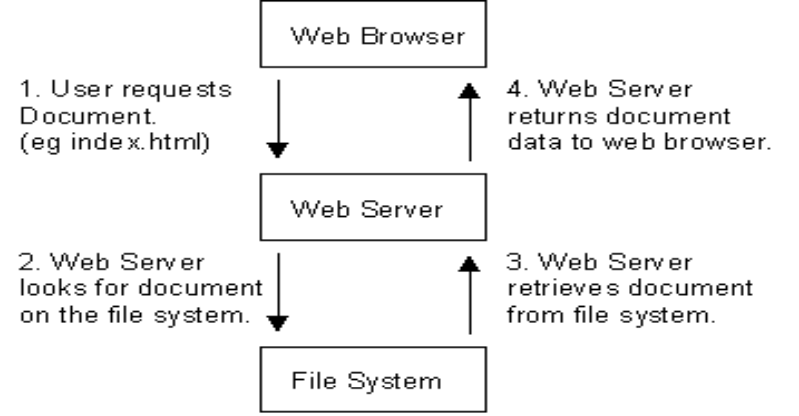
\includegraphics[scale=0.5]{content/images/webserver.png}
	\caption{How web servers and web browsers work illustrated \cite{webserver}}
	\label{fig:webserver}
\end{figure}

%ajax Eventlere bagliyor http requestleri javascript kullanarak. jQuery de isleri kolaylastirmak icin
The following technologies have been used in order to create dynamical webpage:
\begin{itemize}
	\item \textbf{HTML:} This markup language is used for defining how body elements are located in a web page and including scripts.
	\item \textbf{CSS:} CSS is used for defining the style of body elements. Borders, background properties, colors, button styles, positioning of elements are defined with CSS language.
	\item \textbf{JavaScript:} The JavaScript language is used for defining animations, as well as how events would behave.
	\item \textbf{jQuery:} jQuery \cite{jquery} is a JavaScript framework that is written using JavaScript which helps to use define scripts easier than it is with the JavaScript. It is open-source and widely used in almost every web page.
	\item \textbf{AJAX:} AJAX \cite{howajaxworks} is another framework for JavaScript which is used for handling dynamical HTTP requests without having to refresh the page. With the objects it delivers, events such as key press, mouse events, conditional events could be sent to server and processed. The returned data could be processed using JavaScript in order to dynamically update the page content \cite{howajaxworks}. This mentioned working principle is illustrated in the Figure \ref{fig:ajaxpng} \cite{howajaxworks}. 
	\begin{figure}[!ht]
		\centering
		\captionsetup{justification=centering}
		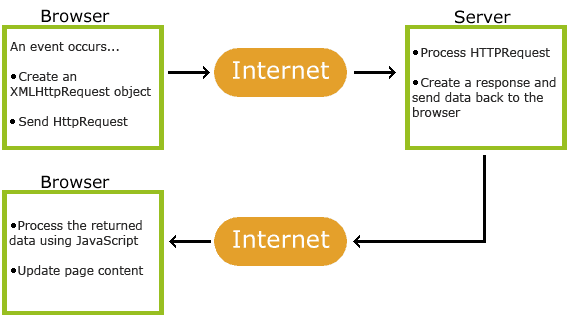
\includegraphics[scale=0.7]{content/images/ajax.png}
		\caption{How AJAX works \cite{howajaxworks}}
		\label{fig:ajaxpng}
	\end{figure}
\end{itemize}

\subsubsection{Web Page Design and Implementation} 
The web page that has been designed for users is shown in the Figure \ref{fig:web}. In the web page, it is seen that a camera stream, control buttons and sliders, and an information graph that shows core utilization in both high-level and low-level module are embedded. For the static design of the web page HTML and CSS are used, while the dynamical behavior of the web page is supported with jQuery, AJAX, and Python. The dynamical behavior of the individual parts of the web page will be explained in the following sections.
\begin{figure}[!ht]
	\centering
	\captionsetup{justification=centering}
	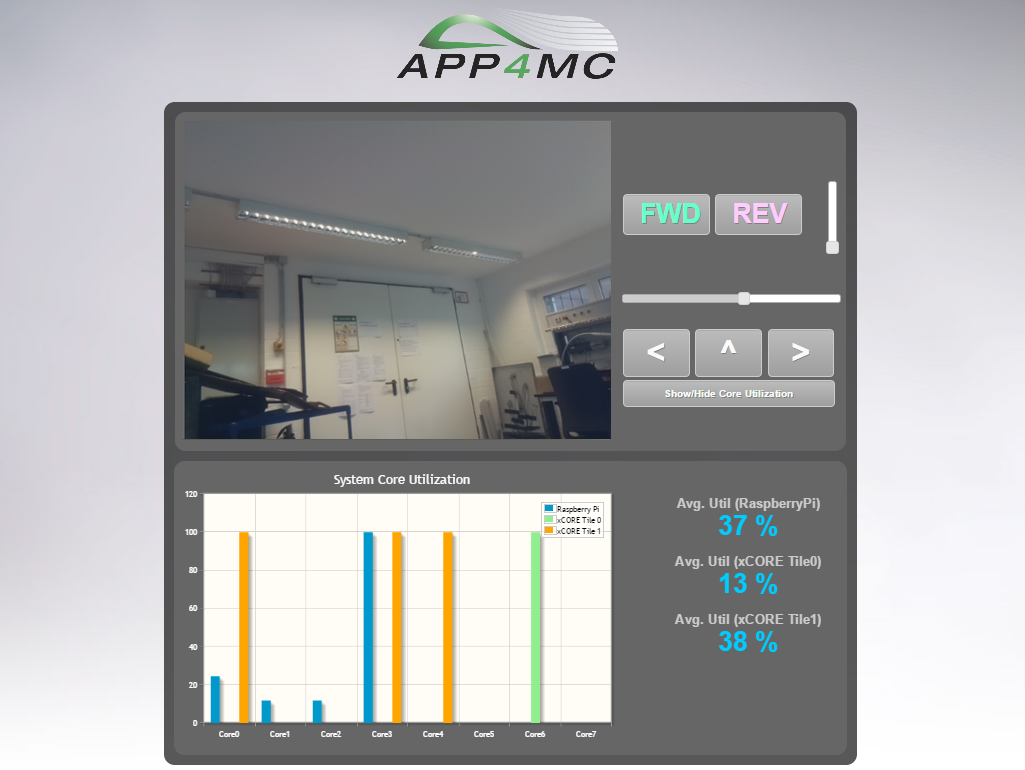
\includegraphics[width=\textwidth]{content/images/web.png}
	\caption{Web interface of A4MCAR}
	\label{fig:web}
\end{figure}

An alternative to this interface have also been created which is used for smoother driving by using arrow buttons. However, the interface that uses buttons can use only constant speeds for actuation which are set to 80 percent of the full speed. The alternative interface can be seen in Figure \ref{fig:web2}

\begin{figure}[!ht]
	\centering
	\captionsetup{justification=centering}
	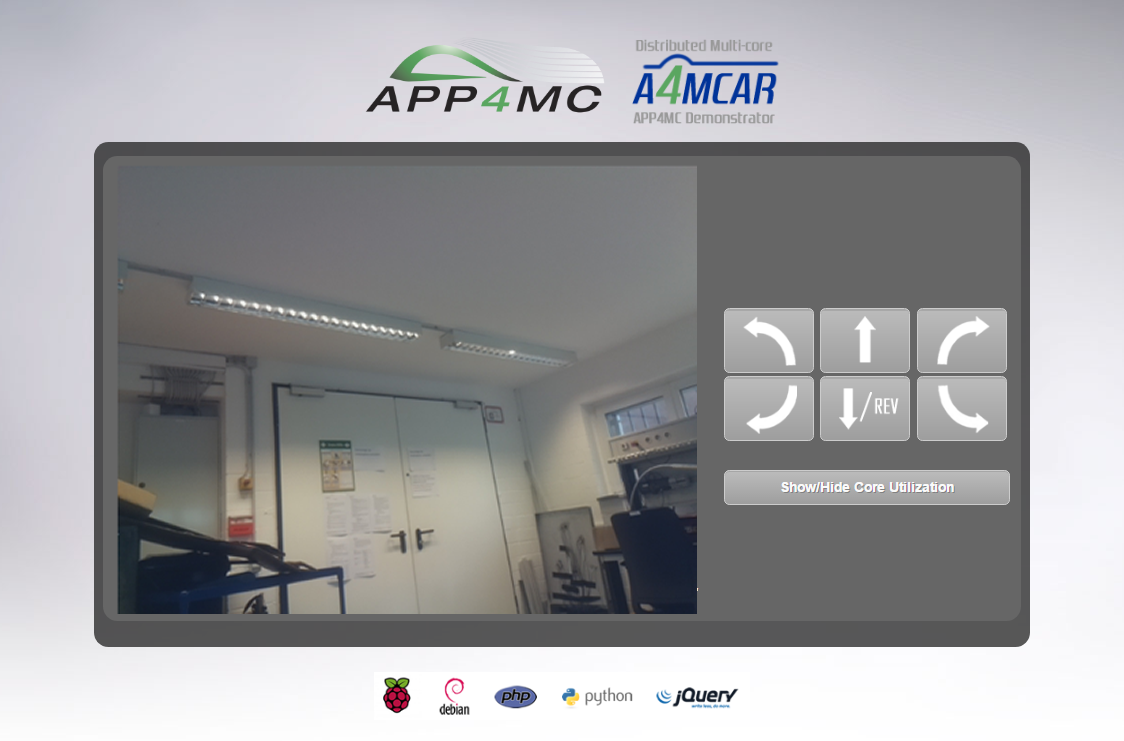
\includegraphics[width=\textwidth]{content/images/web2.png}
	\caption{Alternative web interface of A4MCAR}
	\label{fig:web2}
\end{figure}

The overall dynamical behavior of the web page is illustrated in component diagram that is seen in the Figure \ref{fig:weboverallbehavior}. In the diagram, it should be noticed that the server page jqueryControl.php is the main web interface. It has some server pages and files embedded to it in order to function as a whole to deliver the features of controlling A4MCAR, core utilization display, and camera streaming. In the following subsections, each of these tasks will be explained using the component diagram shown in the Figure \ref{fig:weboverallbehavior}.

\begin{figure}[!ht]
	\centering
	\captionsetup{justification=centering}
	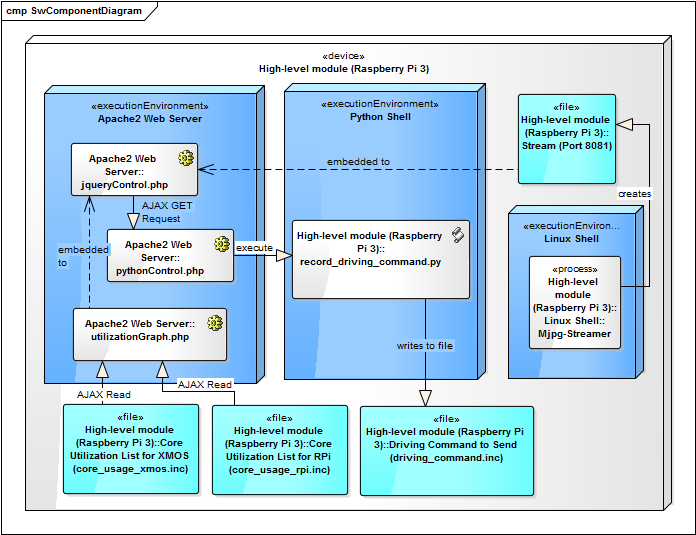
\includegraphics[width=\textwidth]{content/images/weboverallbehavior.png}
	\caption{Component diagram showing how communication inside the created web-interface works}
	\label{fig:weboverallbehavior}
\end{figure}

\subsubsection{Controlling A4MCAR via Web Page}
At the top right of the Figure \ref{fig:web}, the controls to drive the A4MCAR over web interface is shown. It is seen that there are gear selection buttons such as Forward (FWD) and Reverse (REV), along with two sliders. The sliders are created using the third party script library called 'jquery\texttt{\_}ui'. While the vertical slider is for speed adjustment, the horizontal slider is used for angle adjustment. Additionally, to select the very left, straight, and very right angles the arrow buttons could be used. 

With the help of jQuery and AJAX' ability to create event handlers within server pages, on a button press or when slider position is changed, an event handler is run that collects the position and gear information and sends it using an HTTP "GET" request dynamically to another server page called pythonControl.php (shown in Figure \ref{fig:web}). With the idea of demonstrating a basic AJAX request, an example of this is given in the Listing \ref{lst_ajax}.

\lstinputlisting[caption=Sending dynamic HTTP GET requests using jQuery , label=lst_ajax, style=jquery]{content/listings/lst_ajax.txt}

As it is seen from the Listing \ref{lst_ajax} url field, the information that is sent is nothing other than the format defined for the bluetooth communication in the low-level module, which is given in \ref{fig:bluetoothcommand}. In the Figure \ref{fig:web}, it is seen that after the information is received by pythonControl.php, using the ability of PHP to run a shell script, a Python script is run using the Python shell automatically. The python script, whenever executed, writes the received driving command information into the text file that holds the driving command. This operation is done asynchronously. How the driving command is sent afterwards is explained in the Section \ref{llethsection}.
\subsubsection{Camera Streaming}
For the camera streaming, the third party module mjpg-streamer \cite{mjpgstreamergithub} has been used. This module is able to communicate over CSI interface in order to generate a stream on a network port, which then could be embedded to web pages. It is seen on the Figure \ref{fig:weboverallbehavior} how this module works along with the Apache2 Web Server. 

For the stream, Raspberry Pi camera version 2.0 with CSI interface is used which is shown in the Figure \ref{fig:rpicam20}.

\begin{figure}[!ht]
	\centering
	\captionsetup{justification=centering}
	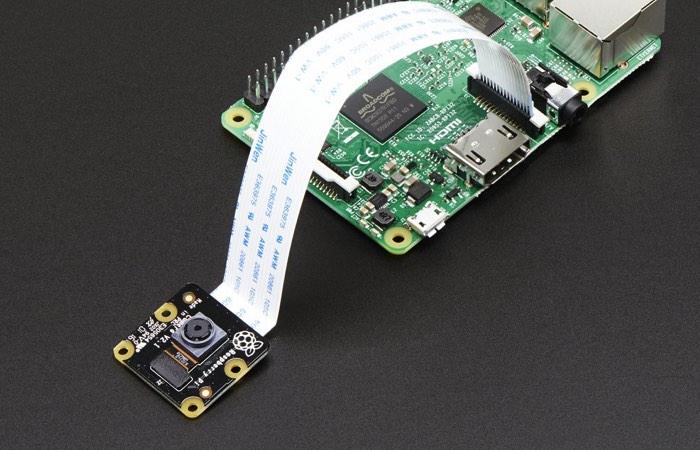
\includegraphics[scale=0.5]{content/images/rpicam20.jpg}
	\caption{Raspberry Pi camera v2.0}
	\label{fig:rpicam20}
\end{figure}

Based on the documentation of the mjpg-streamer, a script using Bash language is created which is used for generating a web stream with the correct parameters. These parameters involve resolution, frames per second, quality value, and port on which the stream will be generated. For the case of A4MCAR, the experimental version of mjpg-streamer has been used which is able to stream using the Raspberry Pi camera besides a webcam. By using the experimental version library, the following setup is found to give robust performance:
\begin{itemize}
	\item Resolution:        640x480
	\item Frames per second: 30
	\item Quality:           default
	\item Port:              8081
\end{itemize}
\subsubsection{Core Utilization Display}
Core utilization display is shown at the bottom of the Figure \ref{fig:web}. It is responsible for gathering all the core usage information from the files, displaying a graph showing percentages, and calculating average core utilizations. These operations are handled within the server page utilizationGraph.php as shown in the Figure \ref{fig:weboverallbehavior}. This server page is embedded into the main web interface which is jqueryControl.php.

For the efforts regarding creating a graph, a third party script library called 'jqPlot' \cite{jqplot} which runs within the jQuery framework is used.  The jqPlot offers various functions in order to create various plots such as bar graphs, line graphs, pie charts and 3D plots. In order to embed the plots into the web page, AJAX has been used.

\subsection{Dummy Loads}
In order to fully utilize the developed parallel software on the high-level module under full load, several processes have been created which do dummy operations to use a certain percentage of the cores. Although the initial distribution does not involve dummy load processes due to increased responsiveness, the dummy loads is used for stressing the software. To create dummy loads, two ideas are investigated:
\begin{itemize}
	\item \textbf{Basic load with very short periods:} While using this methodology achieves certain core percentage loads, having a very short delay is considered to be non model-safe and since periods of the processes are very short, timing logs resulted in deadline misses for further analysis. Therefore, a new method of using bigger load with bigger periods is analyzed.
	
	\item \textbf{Bigger load with bigger periods:} While using a bigger load with bigger period is also viable in achieving certain core percentages, the fluctuation in the core utilization values higher than the previous option. This fluctuation is trivial in our application as most of the processes behave this way.
	
	\lstinputlisting[caption=Dummy load created with Python , label=lst_dummyload, style=python]{content/listings/lst_dummyload.txt}
	
	In order to create the dummy loads in the code, matrix multiplication of random 1000 by 1000 matrices is processed. Python offers libraries to create those matrices as well as to multiply them. The basic load that is written in Python is given with the Listing \ref{lst_dummyload}.
	
	While various loads with the same matrix operation are created, it should be noted that they differ in their iteration periods which helps to achieve different core utilization percentages. The Table \ref{tbl_dummyloads} is a list of all dummy processes that are created in order to help with the utilization research:
	
	\begin{table}[h!]
		\begin{tabular}{|l|l|l|l|}
			\hline
			Process Name & File Name & Period & Core Utilization \\
			\hline
			\hline
			CycleWaster25\texttt{\_}1 & dummy\texttt{\_}load25\texttt{\_}1.py & 1.4 second & 25 percent \\
			\hline
			CycleWaster25\texttt{\_}2 & dummy\texttt{\_}load25\texttt{\_}2.py & 1.4 second &  25 percent \\
			\hline
			CycleWaster25\texttt{\_}3 & dummy\texttt{\_}load25\texttt{\_}3.py & 1.4 second &  25 percent \\
			\hline
			CycleWaster25\texttt{\_}4 & dummy\texttt{\_}load25\texttt{\_}4.py & 1.4 second &  25 percent \\
			\hline
			CycleWaster25\texttt{\_}5 & dummy\texttt{\_}load25\texttt{\_}5.py & 1.4 second &  25 percent \\
			\hline
			CycleWaster100 & dummy\texttt{\_}load100.py & 0.50 second & 100 percent \\
			\hline
		\end{tabular}
		\caption{Dummy load processes running in high-level module}
		\label{tbl_dummyloads}
	\end{table}
	
\end{itemize}

\subsection{Image Processing with OpenCV}
Developing cyber-physical systems with multiple sensors require a good knowledge of computer vision. Automotive applications especially when developing Advanced Driving Asistance Systems (ADAS) make use of this knowledge. Huge computational power need involved in such applications makes such processes a challenge. Therefore, a demonstration of an image processing application is crucial in A4MCAR.

For demonstration of parallelization of an image processing process along with several other processes and threads, an application that can roughly detect a traffic cone has been developed using the C++-based and well established computer vision library OpenCV \cite{opencv}. The developed application makes use of Raspberry Pi camera (using 'raspicam' library) to retrieve images and performs several transforms to the image to detect traffic cones. The developed application outputs an "OBJECT FOUND" message to demonstrate its operation. An example of detections are given in the Figure \ref{fig:traffic_cone_detection}.

\begin{figure}[!ht]
	\centering
	\captionsetup{justification=centering}
	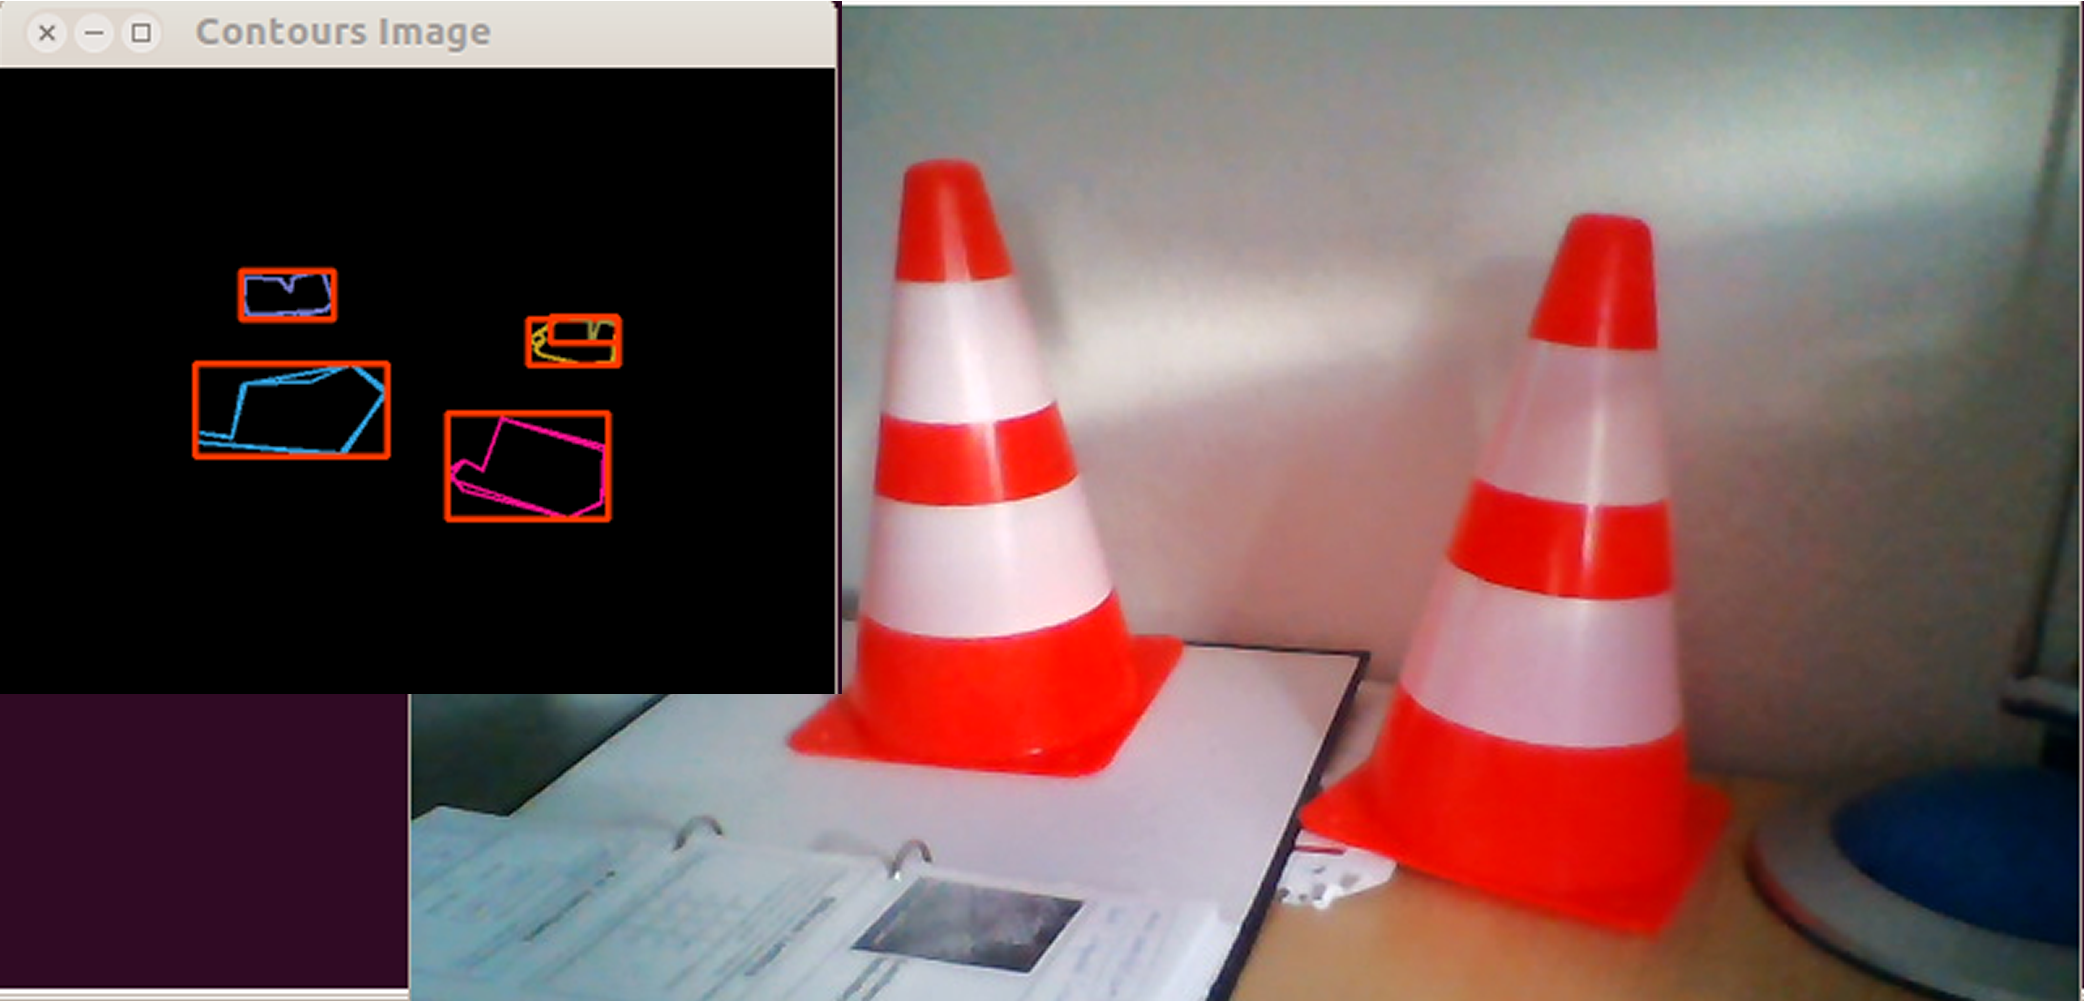
\includegraphics[scale=0.15]{content/images/traffic_cone_detection.png}
	\caption{Developed Image Processing Application}
	\label{fig:traffic_cone_detection}
\end{figure}

The applied transformations and how the traffic cone is detected as demonstration is illustrated with the Figure \ref{fig:imageproc}. The idea that is depicted is to retrieve contours of the possible objects and then determining whether it is a traffic cone or not by filtering those contours by their sizes and aspect ratios. In the figure, it is seen that several transformations are applied for this purpose. Creating the threshold image and then subtracting the background (steps: Background AND, Flood Fill, Image Inversion, Bitwise OR), the image is prepared for the canny edge detection step. Canny Edge Detector, i.e. 'Canny' function is able to find edges of desired objects. By using edges, contours can be found which represent the outlines of objects. By judging the contours on their sizes and aspect ratios the desired objects are detected.

\begin{figure}[!ht]
	\centering
	\captionsetup{justification=centering}
	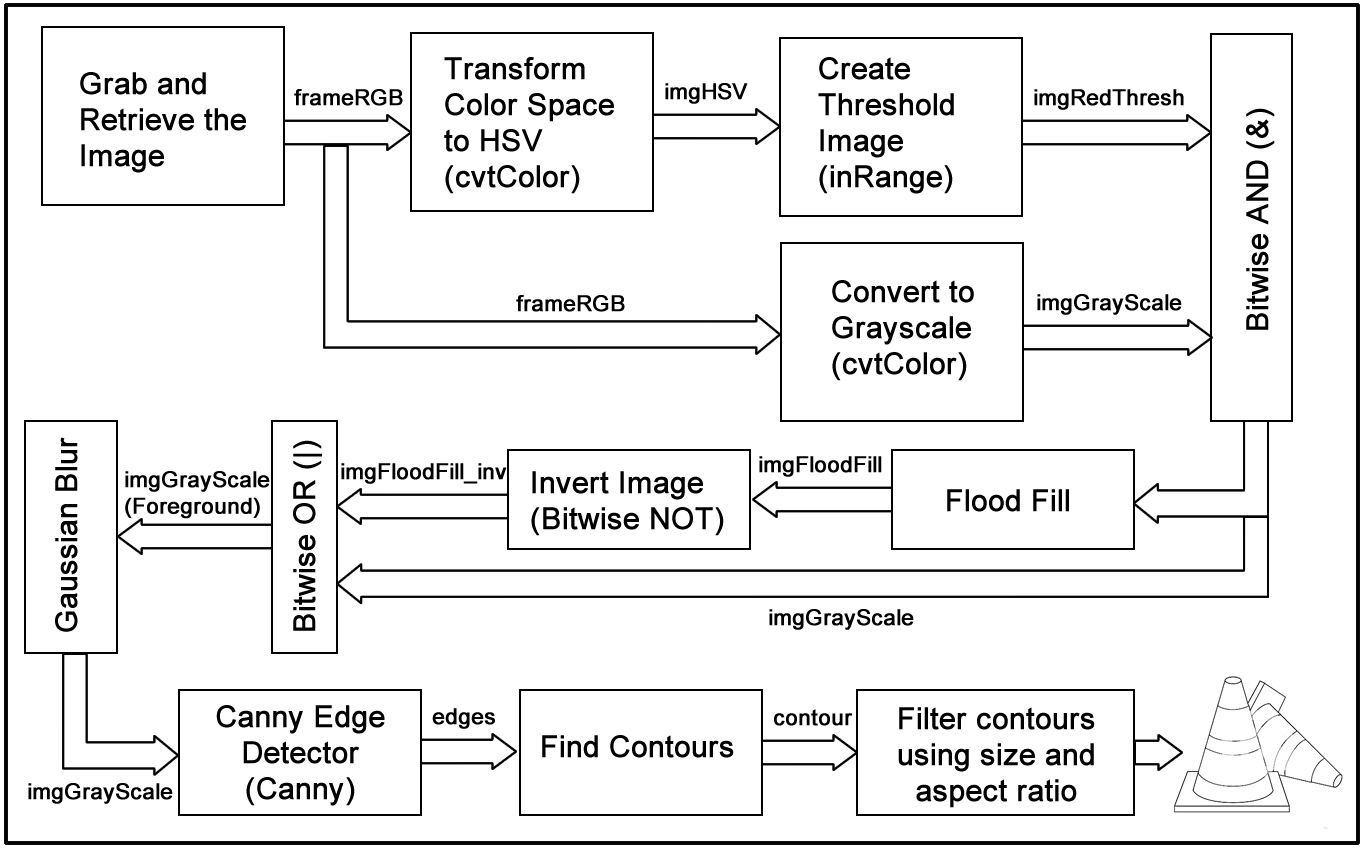
\includegraphics[width=\textwidth]{content/images/imageproc.png}
	\caption{Applied Functions in OpenCV to Detect a Traffic Cone}
	\label{fig:imageproc}
\end{figure}

\subsection{Touchscreen Display}
%Add state machine diagram for display modes
\subsubsection{Touchscreen Display Features}
Touchscreen display that is embedded onto the Raspberry Pi 3 features several functions. It can not only show core utilization graph, average utilization percentages, timing performance, but also can be used to manage and allocate the processes of the high-level module. It also features connectivity settings in order to connect to an access point. Main interface and buttons are shown in the Figure \ref{fig:displaybuttons}. Using those buttons users can switch between display modes that are mentioned, as well as go to the Settings menu, exit the touchscreen application, and shutdown the Raspberry Pi. 
\begin{figure}[!ht]
	\centering
	\captionsetup{justification=centering}
	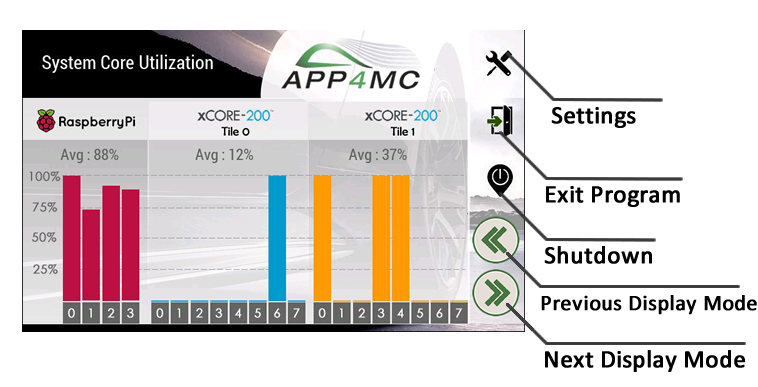
\includegraphics[scale=0.5]{content/images/displaybuttons.png}
	\caption{Button functions of A4MCAR Touchscreen Display}
	\label{fig:displaybuttons}
\end{figure}

\subsubsection{Touchscreen Display Implementation}
 %explain used libraries pygame, psutil and touchscreen interfacing hdmi etc...
%Linux tools and created .sh scripts will be in Section (5)
%Maybe add how graph is made...
As for the hardware, 5 inch HDMI touchscreen module from Waveshare has been used. This module can act as a primary monitor for Raspberry Pi. Addinitionally, the module features touchscreen controls using SPI pins of the Raspberry Pi GPIO. The module driver is installed and calibrated on Raspberry Pi in order to use the module as a primary monitor. 

The touchscreen display process uses a third-party library from Python that is called Pygame \cite{pygame}. This library is exclusively developed for creating Python language based games but it is also useful for creating graphical interfaces. After the images for the interface have been designed, the main interface has been created using the functions from Pygame. As an example, one page is designed to show the system core utilization. In that page, visualization is handled by creating rectangles that scale from 0 percent to 100 percent to show the core utilization in each core that are obtained by reading the files that are responsible for holding the core usage information for both low and high level modules.
\begin{figure}[!ht]
	\centering
	\captionsetup{justification=centering}
	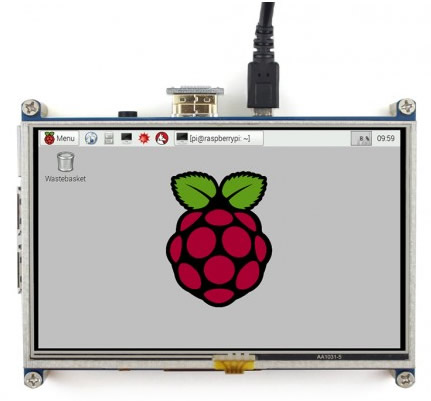
\includegraphics[scale=0.6]{content/images/touschreen5inc.jpg}
	\caption{5 inch Touchscreen module from Waveshare}
	\label{fig:touschreen5inc}
\end{figure}

Pages that are developed for the touchscreen module are shown in the Figure \ref{fig:displays}. In order to understand the behavioral operation of the touchscreen process, the Figure in \ref{fig:TouchscreenProcessSM} should be observed in parallel with the Figure \ref{fig:displays}. 
\begin{figure}[!ht]
	\centering
	\captionsetup{justification=centering}
	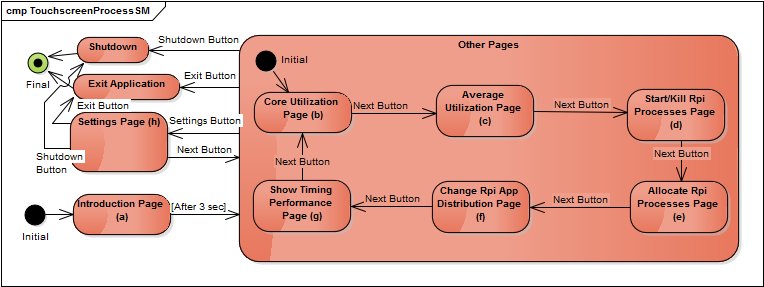
\includegraphics[width=\textwidth]{content/images/TouchscreenProcessSM.png}
	\caption{State machine of touchscreen process for pages as modes}
	\label{fig:TouchscreenProcessSM}
\end{figure}
\begin{figure}[!ht]
	\centering
	\captionsetup{justification=centering}
	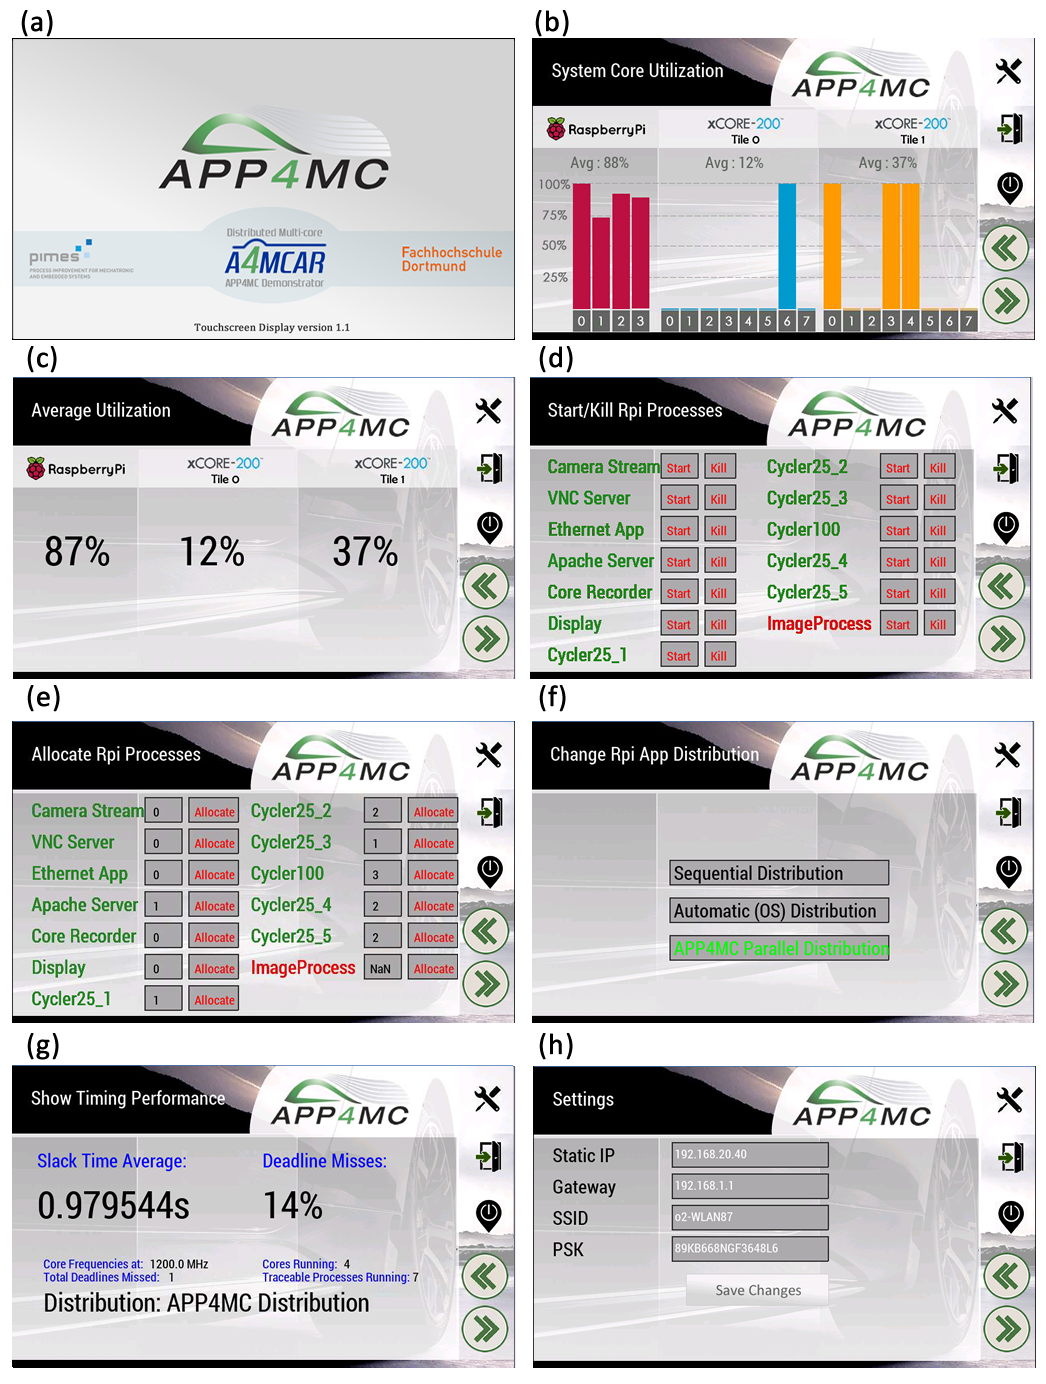
\includegraphics[width=\textwidth]{content/images/displays.png}
	\caption{Display modes from A4MCAR Touchscreen Display}
	\label{fig:displays}
\end{figure}

The introduction page that is shown in Figure \ref{fig:displays} (a) is entered as the process is started. After displaying the logo for 3 seconds, other pages are entered. The pages (b) through (g) (shown in Figure \ref{fig:TouchscreenProcessSM}) is navigated with the help of the Next and Previous button in this state. Users can browse the settings page, shutdown or exit the touchscreen display process by clicking to the respective buttons.

In order to make the the touchscreen display software modular, a class that is called 'aprocess' has been created. By instantiating 'aprocess' objects and appending them to the object list 'aprocess\texttt{\_}list', one can define the processes or threads that will be displayed and traced. The touchscreen display software is designed in the modular fashion that it automatically generates all the pages using the aprocess object list. 'aprocess' class have the following attributes and functions to make process handling easier in Python-based software:

\begin{itemize}
	\item \textbf{Attributes:} Process Name (\texttt{apname}), Process ID (\texttt{apid}), Running flag (\texttt{aprunning}), Core Affinity (\texttt{aaffinity}), Command to start the process (\texttt{apstartcommand}), Traceable flag (\texttt{traceable}), Online tracing log file (\texttt{aplogfilepath}), Displayed flag (\texttt{displayed}), Display name (\texttt{display\_name}), Flag to tell if it is a process or a thread (\texttt{is\_thread})
	\item \textbf{Functions:} \texttt{UpdateProcessIDAndRunning()} function is used to update the object process ID and whether the process is running. \texttt{UpdateProcessCoreAffinity()} function is used to retrieve the process core affinity while the  \texttt{SetCoreAffinity(core\_affinity)} function is used for setting the core affinity. There are also thread-specific methods such as \texttt{SetCoreAffinityOfThread(core\_affinity)} and \texttt{UpdateThreadIDAndRunning()}.
\end{itemize}

Touchscreen display process have a multi-threaded design. In this design Python's threading library \cite{pythonthreading} has been used. With Python's threading library, one can create threads and handle the shared memory communication between threads. The aforementioned process and thread list, 'aprocess{\_}list' is protected by using the mutex implementation 'Lock()' \cite{pythonthreading} of Python's threading library. The following listing shows how locking works with Python's threading library:
\begin{lstlisting}[style=python]
lock.acquire()
# Access to the shared variable
lock.release()
\end{lstlisting}

In the implementation of the touchscreen application, the display resulted in problems due to non-locked access to 'aprocess{\_}list' variable. The concurrent write and reads to this shared variable therefore is prevented using 'Lock()'.

Initial implementation of the touchscreen display did not involve any threads. However, that resulted in several problems. The most crucial problem that occured by not having a multi-threaded design was that in order to make the processes schedulable (explained in the Section \ref{onlinetiming}), the responsiveness of the touchscreen would drop significantly since each display mode has different periods due to embedded calculations. By isolating the calculations, touchscreen events, and utilization updates, this problem is resolved. The four threads that touchscreen display has can be listed as follows:

\begin{itemize}
	\item \textbf{Main Thread:} Responsible of solely displaying the information using shared variables
	\item \textbf{TimingCalculation Thread:} This thread is responsible of reading from all the timing log files that are registered to the application using 'aprocess' class, and calculating the values such as gross execution time, slack time average, deadline misses, traceable processes running.
	\item \textbf{TouchscreenEvents Thread:} Pygame library provides all event handling within a loop. Therefore, it is unwise to handle it without a thread, in case there are many events to be checked. For that purpose, TouchscreenEvents thread is created. The thread is able to emit events in case there is a mouse click or key press.
	\item \textbf{UpdateUtil Thread:} This thread is able to read from core utilization log files and parse the information to update shared variables so that the Main Thread could show the results.
\end{itemize}

For the sake of informational completeness, how the schedulable Python threads are created should be depicted. Therefore, the Listing given in \ref{lst_threadskeleton} should be explained.

\lstinputlisting[caption=Thread skeleton in Python, label=lst_threadskeleton, style=python]{content/listings/lst_threadskeleton.txt}

In the Listing \ref{lst_threadskeleton}, a schedulable dummy thread is skeleton is shown. Between lines 2 through 4, the shared variables are defined. Lines 7 shows instantiating an 'aprocess' object by entering thread name, traceability, log file, displayability, display name, starting command, and whether or not if it is a thread, respectively. In the line 8 and line 9, thread ID is updated and the core affinity of the thread is set. Lines 10 through 12 shows globally updating the 'aprocess{\_}list' with the created thread by making use of mutexes. Between lines 16 and 24, the schedulability and traceability features are implemented which was discussed in the Section \ref{onlinetiming}.

Since the touchscreen display process is responsible from displaying many information, libraries to gather up such information have been used. Furthermore, the data that is gathered in the timing logs and core usage logs have also been used in this application. Information that is gathered involve core usage percentages of both low-level and high-level modules, slack times of high-level processes, core frequency of high-level module, active cores count for the high-level module and core mapping list from the high-level module. There is also ability to change the core frequency (Figure \ref{fig:displays} (g)), and display gross execution time. The detailed information on how the timing information is extracted will be explained in the Section \ref{informationchapter}.

\subsection{VNC Server}
Virtual Network Computing (VNC) is a system that allows creating and managing virtual computers as well as connecting to them remotely \cite{vncmagazine}. While dealing with programming single board computers such as Raspberry Pi, it is used for viewing the single board computer desktop remotely. During the development of A4MCAR, a third-party application called XtightVNC is installed to both the Raspberry Pi and the development computer in order to connect to it without having to use external hardware.  The VNC server that is installed in Raspberry Pi, XtightVNC, is run at boot time and scheduled like any other process on the Raspberry Pi. While the server has not been manipulated during the development, in order to investigate the parallelism efficiency, this third party application should also be considered in order to get more accurate results. Further information regarding parallelism findings will be given in Chapter \ref{informationchapter} and Chapter \ref{evaluationchapter}. 

\section{Android Application Implementation}
To control the A4MCAR remotely via communicating with the RN42 bluetooth module that is connected to the low-level module, A4MCAR control application is developed using Android \cite{androidwebsite} environment. In the Figure \ref{fig:tasksoverall}, one can see how developed A4MCAR control application interacts with the entire software that is developed for A4MCAR. 

As an integrated Android development environment, Android Studio \cite{androidstudio} is used. Using Android Studio, developers can not only design XML-based user interfaces for their applications, but also can describe the behavior of their programs using Java programming language. Additionally, Android Studio can emulate many of the available Android devices to help the developers debug their software. 

The developed Android application interface is given in Figure \ref{fig:androidapp}. In the figure, it is seen that the interface consists of a joystick and gear buttons that helps in constructing the driving command that was given by the Figure in \ref{fig:bluetoothcommand}. Furthermore, using a bluetooth device list, A4MCAR could be paired with and then connected in order to start data communication.

For the joystick controls, a third-party Android library that is called virtual-joystick \cite{virtualjoystick} is used. Using this library, one can import the joystick mechanism into their applications. In order to handle the data created from the joystick, an on move event handler has been created which is a callback function which acts every time the joystick is moved. Using this callback function, the angle and strength information that results from the joystick has been transformed to conform to the driving command (Figure \ref{fig:bluetoothcommand}). With the help of the Figure \ref{fig:joystickpie}, this data transformation can be explained easily.
\begin{figure}[!ht]
	\centering
	\captionsetup{justification=centering}
	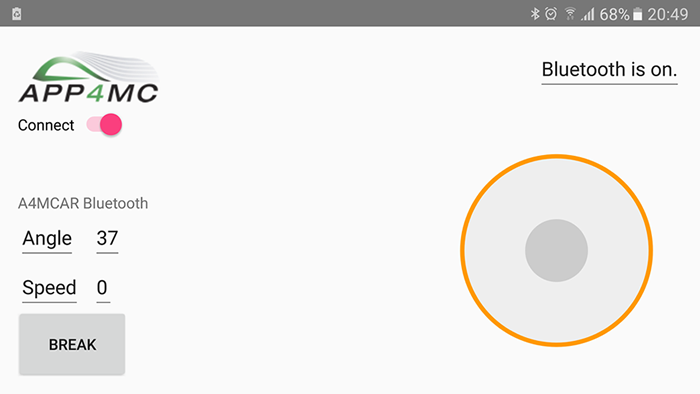
\includegraphics[scale=0.6]{content/images/androidapp.png}
	\caption{Android Application Developed for Driving A4MCAR Remotely}
	\label{fig:androidapp}
\end{figure}
\begin{figure}[!ht]
	\centering
	\captionsetup{justification=centering}
	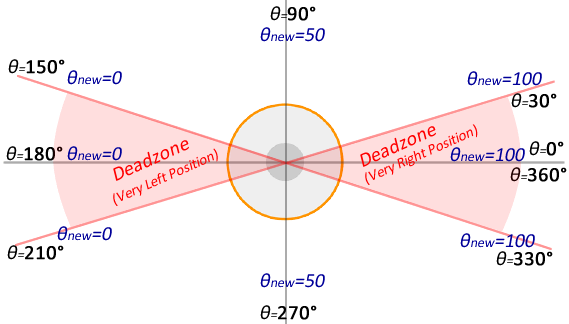
\includegraphics[scale=0.6]{content/images/joystickpie.png}
	\caption{Joystick angle transformation to construct driving command}
	\label{fig:joystickpie}
\end{figure}

Using the joystick illustration given in a Cartesian coordinate system, the angles that are generated by the joystick library itself $\theta$ (0 to 360 degrees) have been converted to the angles for the driving command format $\theta\textsubscript{new}$ (0 to 100). Although the transformations are made to the values from 0 to 100, later on this is reduced to the values from 0 to 99 in order to get rid of the 3-digit format which is not accepted by the command parser written in the low-level module side.

As it is clearly shown in the Figure \ref{fig:joystickpie}, there are certain dead zone regions on the joystick which are not taken into account in the transformation for the sake of the comfort of the users. While the transformed angle $\theta\textsubscript{new}$ is  constant in the dead-zone regions, a few equations have been used in order to handle the mapping of angles in the remaining regions:
\begin{itemize}
	\item If the angle is between 30 degrees and 150 degrees, the transformed new angle is calculated using the following:
	\begin{equation}
	\theta\textsubscript{new}=\left(1 - \frac{\theta - 30}{120}\right) 100
	\end{equation}
	\item If the angle is between 210 degrees and 330 degrees, the transformed new angle is calculated using the following:
	\begin{equation}
	\theta\textsubscript{new}=\left(\frac{\theta - 210}{120}\right) 100
	\end{equation} 
\end{itemize}
After the calculations, with the current gear setup the data is sent to the low-level module using the bluetooth functionality of the Android application.
%%% CHAPTER A4MCAR ------------------------------------end----


%%% CHAPTER Information Tracing and System Management --------begin----
\chapter{Information Tracing and System Management} \label{informationchapter}
\section{Introduction}
After the distributed multi-core system is developed and defined, the evaluations regarding different software distributions are needed in order to parallelize the system efficiently. For that purpose, one should know how to manage the multi-core system. While managing the system is quite important to maintain and properly optimize the system to its full capabilities, one requires information regarding the system itself in order to achieve this optimization. As an example, the textbook methodology of extracting useful information from a software is to analyze online and offline trace of the system. 

In order to obtain information regarding a software such as number of instructions, how tasks are scheduled, timing details regarding tasks, core frequencies, energy consumption rates, the following techniques are mostly used:
\begin{itemize}
	\item \textbf{Static Binary Analysis:} Static binary analysis is a reverse engineering methodology that helps in finding errors in code such as the errors that involve non-determinism \cite{staticanalysisPRE}. It is essentially analyzing the binaries that are created from C and C++ programs to have another approach to traditional error finding methodologies such as testing and code inspection \cite{staticanalysisPRE}. It is important to keep in mind that in the static binary analysis, the program is not executed \cite{dynamicanalysisphd}. Therefore, the information regarding execution and timing are not provided while the instruction information could be extracted. However, it should be noted that some processor or platform specific tools can estimate the timing based on the number of instructions and the processor information. With the static binary analysis, the disassembly information which is the list of all the instructions could be observed. With the help of the binary analyzer tools, detailed information on number of function calls, nesting, and cyclic complexity could be observed \cite{staticvsdynamicanalysis}. %cyclomatic complexity.
	%this is simply observing disassembly
	\item \textbf{Profiling (Dynamic Analysis):}
	Dynamic analysis, also called profiling, is the methodology of analyzing the program by considering its execution in contrast to the static binary analysis \cite{dynamicanalysisphd}. Dynamic analysis is often done by using tools and it is done in order to get information of how a program is executed on a real or virtual processor \cite{staticvsdynamicanalysis}. While dynamic analysis is quite useful for identifying vulnerabilities in a runtime environment and obtaining information such as timing of execution, it can not guarantee the full test coverage of the source code \cite{staticvsdynamicanalysis}. Using dynamic binary instrumentation (DBI) tools for Linux platform this way, one can obtain information such as CPU time, execution times, memory and I/O of a program \cite{dynamicanalysisphd}. 
	\item \textbf{Tracing:} Tracing is a methodology which is often mixed with profiling. According to IPM \cite{IPM}, a trace records the chronological information of the execution of a program or a system via logging the the execution with timestamps, whereas a profile is the collection of performance events and timings for a program's execution as a whole. Therefore, it can be said that the scheduling of an Operating system could be analyzed with the help of tracing. 
	
	The A4MCAR involves tracing features that are not only supplied by Linux tools but are also developed within the project. It can be generalized that online tracing is a type of tracing that is done while the program is being executed using buffered logs while offline tracing is done after the program has executed using the entire logs. Regarding this information, it can be said that the developed tracing features are created for online tracing in A4MCAR while the existing tooling is used for offline tracing. The following sections consist of the information regarding tracing developments as well as the tooling support regarding tracing a Linux system.
	\item \textbf{System Monitoring:} Unlike static binary analysis and profiling, system monitoring \cite{systemmonitoring} is done within the entire system and it is used for obtaining useful information regarding the system performance as a whole. Operating systems (especially Linux platform) usually have system logs which could be observed via system monitoring in order to extract useful information regarding the system performance. Speaking for A4MCAR, the performance values such as core frequency and core utilization information are extracted using system monitoring.
	%We did this with psutil, also proc folder
\end{itemize}

%Here comes our motivations
%What kind of information needed?
%Why?
%In APP4MC
%Why do we do this?
%In both low and hight level modules
%This chapter will involve....
Low-level and high-level modules of A4MCAR requires several information. To start with, in order to model the software system of both modules with A4MCAR, the number of instructions, task iteration periods, and if exists event occurrance types are needed. This could be achieved by using static binary analysis method in the low-level module due to the fact that XTA tool can estimate instructions, timing, and path from the static binary analysis. The information of number of instructions and periods are obtained from the high-level module Linux platform by using tools that perform profiling. Although using a static binary analysis tool is possible, using a profiler tool was selected as the option for easement of the process. Secondly, system monitoring is needed in both of the modules. While the system monitoring is done using registers in the memory for the low-level module, it is achieved by using Linux kernel tools in high-level module. System monitoring in A4MCAR is essentially needed in order to obtain core utilization percentages, live CPU frequency and active core count. Finally, the profiling and tracing of the programs of the high-level module is needed in order to evaluate parallelization performance and visualize how processes are scheduled. The data that are obtained from profiling and tracing involve slack time, execution times, start and end times.

In this chapter, the aforementioned techniques for system analysis will be discussed with the emphasis of their applicability on a real distributed multi-core system that involves elements from a low-level multi-core micro-controller and a high-level single board computer that is running on x86/Linux platform in order to elaborate  modeling, managing, profiling, tracing of systems and evaluation of various software distributions.

\section{Low-Level Module Information Tracing and System Management}
\subsection{Static Binary Analysis via XTA} \label{staticbinary}
XMOS Timing Analyzer (XTA) \cite{xtamanual} is an Eclipse-based tool that comes with xTIMEcomposer platform which is used for analyzing the timing and the execution details of the multi-tasked software that are developed using XMOS boards and processors \cite{xtamanual}. The tool is able to measure shortest and longest time required to execute a section of code by analyzing the binary file. Thus, the code is not executed in order to be analyzed. Furthermore, it is also able to check the minimum and maximum number of instructions required to execute a section of the code.  A screenshot from the XTA tool is given in the Figure \ref{fig:xtass}.

\begin{figure}[!ht]
	\centering
	\captionsetup{justification=centering}
	\includegraphics[width=\textwidth]{content/images/xtass.png}
	\caption{XMOS Timing Analyzer (XTA) screenshot}
	\label{fig:xtass}
\end{figure}

Once the code is written and built in xTIMEcomposer platform, a binary file is generated with the extension .XE. By loading this binary file using XTA, the timing analysis could be performed. In order to load the binary to XTA, "Load Binary" button (shown as 1 in the Figure \ref{fig:xtass}) should be pressed. Once the binary is loaded, the Disassembly window (shown as 4) appears which shows all the runnables that are automatically detected from the binary. Using the disassembly window, the instructions that are used in runnables could be seen. 

XTA tool is also able to work with specific commands by using the XTA console (shown as 5). Using the specific commands taken from XTA manual \cite{xtamanual}, timing analysis could be done easily. In order to start timing analysis, an execution path should be defined. The execution path could be determined analyzed using the following possible ways \cite{xtamanual}:

\begin{itemize}
	\item Via placing end points into the code using compiler directive \texttt{\#}pragma as shown in the Listing \ref{lst_xtaendpoints}.
	\lstinputlisting[caption=Placing end points in xC code to define execution path , label=lst_xtaendpoints, style=xc]{content/listings/lst_xtaendpoints.txt}
	The timing analysis between two endpoints could be started by entering the following command to the XTA console:
	\begin{lstlisting}[style=xc]
	analyze endpoints start_endpoint1 stop_endpoint1
	\end{lstlisting}
	\item A function or a runnable with the name "Function\texttt{\_}Name" could be analyzed from its starting point to its return point by using the following command:
	\begin{lstlisting}[style=xc]
	analyze function Function_Name
	\end{lstlisting}
	\item Finally, loops can be analyzed using XTA. The way a loop is defined is either setting a loop point from the editor or defining an endpoint inside loop. A loop point having and end point "looppoint" can be analyzed using the following command in the XTA console: \\
	\begin{lstlisting}[style=xc]
		analyze loop looppoint
	\end{lstlisting}
\end{itemize}

The entire code could be modified in the aforementioned fashion in order to do a timing analysis to all of the runnables of the software system. One can set up timing constraints to make sure every dead line is matched \cite{xtamanual}. Once the timing analysis starts, the selected route, i.e. a function, a loop, or a route between two endpoints are shown in the Routes window (shown as 2 in the Figure \ref{fig:xtass}). The selected route is shown in blocks in another window which is shown as 3 in the figure. Here, it is seen that the best case execution time and the worst case execution time of each block is estimated. As an example, for the WriteData function, the best case execution time is estimated to be 3.584 microseconds, whereas the worst case execution time is 432 nanoseconds. Further information that is provided by XTA regarding timing analysis is given in the Figure \ref{fig:xtafurther}. As it is seen in the figure, what kind of timing paths could have been taken for the function can be visualized using the Visualizations window. Furthermore, information such as thread cycles, number of instructions, number of Fnops, and number of paths are also shown.

\begin{figure}[!ht]
	\centering
	\captionsetup{justification=centering}
	\includegraphics[width=\textwidth]{content/images/xtafurther.png}
	\caption{XTA Visualizations window with further information}
	\label{fig:xtafurther}
\end{figure}

For the software that is developed for the low-level module of the A4MCAR, for modeling purposes in APP4MC  the number of instructions are obtained for almost every runnable and event by using aforementioned techniques. For the events, the technique of defining endpoints is used, whereas for the runnables the function analysis is used. However, due to the non-determisim in the some of the branch instructions and code sections that are related to hardware communication, some sections in many runnables were not able to be analyzed properly and returned the "Unresolved" error. In order to get rid of this error, following techniques are used:

\begin{itemize}
	\item The "Unresolved" error occurs usually when XTA can not resolve a branch instruction whose branch target is unknown \cite{xtamanual}. In order to get rid of this issue, trace of the system should be printed and branch instruction target should be pointed manually. The details of how this is done is given in the XTA manual \cite{xtamanual}. By using this technique, some of the "Unresolved" errors were resolved and number of instructions of those runnables were found.

	\item When the technique above failed to work because of memory instructions such as memset and infinite loops, the number of instructions are gathered by counting the instructions from Disassembly window. Although this technique is time consuming and error-prone, it is assumed that the gathered information is close to the real number of instructions. Additionally, APP4MC partitioning and mapping accuracy would not change drastically if the gathered information is not exact. 
\end{itemize}

In the Section \ref{evaluationchapter}, gathered information along with its implications will be discussed.

\subsection{Distribution of Tasks to Cores}
In a properly utilized parallel system, gathered information are used in order to find which software distribution is the most efficient. Here, the software distribution refers to the mapping stage, which is the distribution of the tasks that result from partitioning to the cores.

In xTIMEcomposer platform, task mapping is done easily with the capabilities of the xC programming language. Since xCORE provides a multi-core platform, using the cores for different tasks can be achieved by using simple statements. Although this is introduced in Section \ref{designchapter}, some of the information will be summarized for completeness sake. In XMOS, placement of a function into a core is done by using "par" statement. In the main block of a software, "par" statement can be used in order to create several tasks in parallel. Additionally, using global interface variables, one can handle the inter-task communication between two parellel tasks.

As opposed to the Listing \ref{lst_howtasksconnectxc}, a simple example would help one better understand how this works using xC:

\begin{lstlisting}[style=xc]
int main(void)
{
	interface my_interface i1;
	par
	{
		on tile[0].core[2] :  Task1 (i1);
		on tile[1].core[3] :  Task2 (i2);
	}
}
\end{lstlisting}

The given code is a basic example of using xC functionality to do a task mapping. The parallel block in the code could be given as the Lines 4 through 8. It is seen that the "Task1" is pinned to the core 2 of tile 0, whereas the "Task2" is pinned to the core 3 of the tile 1. Furthermore, a global interface of type "my\texttt{\_}interface" having the name i1 is declared in the Line 3. This interface handles the communication between the tasks "Task1" and "Task2". As mentioned, the hardware realizes the interface by using the xCONNECT switches to construct a bridge between tiles and cores. Additionally, it should be noted that unlike Raspberry Pi, the tasks are distributed to cores during the reconfiguration in a xC program, i.e where a Task is located can not be changed during run-time due to the nature of xCORE and due to the fact that hardware availability differs from tile to tile \cite{xmosprogrguide}.

By using the aforementioned technique, all the low-level module tasks are distributed to cores at the build-time. 

\subsection{System Monitoring in xCORE}
How cores of the system is monitored in xCORE is discussed in the Chapter \ref{designchapter}. For the sake of completeness, this subsection is dedicated to reminding what is discussed in the Section \ref{coremonitoringsection}. System monitoring is done by polling a system register and finding out if that core is busy or idle at that moment. Referring back to the Listing  \ref{lst_coremonitoring}, how this is achieved could be better understood.

Besides the implemented core monitoring task, XMOS features several more means to monitor the system. First, system could be monitored at build-time using the XTA tool Binary window, Resource Usage tab. In the Figure given in \ref{fig:binaryresourceusage}, it is seen that the information regarding stack memory, program memory, free memory, cores, timers, and channels could be observed in one window using XTA Binary. Another mean to monitor the system is provided by a function called "debug\texttt{\_}printf". As the name of the function suggests, it is essentially a "printf" function to observe your variables. However, "debug\texttt{\_}printf" is a function that does not interrupt inter-process communication and that does not block cores while printing so that developers can monitor without having to worry about so much overhead \cite{xmosprogrguide}.

\begin{figure}[!ht]
	\centering
	\captionsetup{justification=centering}
	\includegraphics[width=\textwidth]{content/images/binaryresourceusage.png}
	\caption{XTA Binary Resource Usage}
	\label{fig:binaryresourceusage}
\end{figure}

Using the "debug\texttt{\_}printf" function, xC-specific tools, a function has been created that helps to find out which function refers to which core. The reason this information is important is because the core ids that are referred with the "par" statements are not the same ids of the core usage implemention. The same issue holds true for the tile ids, as well. By using the following listing, this information could be monitored at run-time:

\newpage\begin{lstlisting}[style=xc]
	int PrintCoreAndTileInformation(char * Function_Name)
	{
		debug_printf("Starting %s task on core ID %d on tile %x\n", Function_Name, 	get_logical_core_id(), get_local_tile_id());
		return 1;
	}
\end{lstlisting}

Here, the get\texttt{\_}logical\texttt{\_}core\texttt{\_}id() is the function to get the real core id from system registers, whereas the get\texttt{\_}local\texttt{\_}tile\texttt{\_}id() function returns the real tile id. This way, we make sure which task uses how many percentage of the core. Once every task is manipulated so that they use this function while the core monitoring is running, system monitoring could be done easily by observing the Console. An example output of the Console from final version of the low-level module software is given with the Figure \ref{fig:finalmonitoring}. It is seen that the core IDs for every task is given and then the core utilization percentages are listed for cores 0 through 7 for each tile.

\begin{figure}[!ht]
	\centering
	\captionsetup{justification=centering}
	\includegraphics[width=\textwidth]{content/images/finalmonitoring.png}
	\caption{System monitoring implemented on xCORE}
	\label{fig:finalmonitoring}
\end{figure}

%%Onceki sectiona ek olarak
%% core_monitoring.xc den bahset
\subsection{Discovering Energy Consumption Features}
One of the most important optimization goals include reducing the energy consumption. To reduce the energy consumption one should have a properly utilized software which is achieved through balancing the CPU load through all the cores of the system. In order to understand this, Power Consumption Application Manual for XS1-L devices \cite{xs1energymanual} should be studied well. 

There are two types of power consumption described regarding a processing unit. Static power consumption describes a chip's power consumption that is caused by the leakage current as the chip is heating \cite{springerparallel}. Therefore, since the leakage current could not be controlled by a user directly, dynamic power consumption, which is the power consumption that is resulted from actual computations, is the concern of our research. The dynamic power consumption of a chip is described by the following equation \cite{dvfspaper}: 
\begin{equation} \label{dyneq}
P\textsubscript{dynamic} = {\alpha} {C\textsubscript{L}} {V\textsubscript{DD}\textsuperscript{2}} {f\textsubscript{clk}}
\end{equation}

We can see from the equation that the power depends on switching probability ${\alpha}$, chip voltage ${V\textsubscript{DD}}$, clock frequency ${f\textsubscript{clk}}$ and collective switching capacitance ${C\textsubscript{L}}$. It is stated in the \cite{springerparallel} that since ${V\textsubscript{DD}}$ linearly depends on the clock frequency ${f\textsubscript{clk}}$, a cubic relationship between power consumption and clock frequency could be observed. The linear relationship between the current ${I\textsubscript{DD}}$ and the frequency is also depicted in the Figure \ref{fig:xs1energy}, showing the performance values for a XS1-L device of XMOS xCORE-200 eXplorerKIT \cite{xs1energymanual}.

%two techniques that power could be reduced..

\begin{figure}[!ht]
	\centering
	\captionsetup{justification=centering}
	\includegraphics[scale=0.5]{content/images/xs1energy.png}
	\caption{XS-1 Power Graph Related to Base Current for an xCORE Core}
	\label{fig:xs1energy}
\end{figure}

In the figure, we see that the base power consumption of one xCORE running an instruction sequence is given with respect to the clock frequency. By looking at the figure, we can see that the internal base current that is related to the operation of xCORE is directly proportional to the clock frequency of the xCORE core. Since the current is directly proportional to the power, as seen by the equation i.e. $P = {I\textsubscript{DD}}  {V\textsubscript{DD}}$, we can conclude that load balancing is one of the most important things to take care of to get a lower frequency thus current in the core, thus reducing the power consumption. It is important to add at this point that power consumption and energy consumption are directly proportional if system is not fully loaded. In other words, decreasing the clock frequency alone is useful to achieve reduced energy consumption in a system in which the load is balanced and there are no deadline misses \cite{dvfspaper}. Using provided internal registers, xCORE core and tile frequencies can be reduced according to the manual \cite{xs1energymanual}. 

It is important to keep in mind that reducing the clock speed is not the only way to reduce the power consumption. If the dynamic switching power is considered rather than the base power consumption, the factors such as operating frequency, amount of communication, and the data itself are all big causes of the power consumption \cite{xs1energymanual}. Therefore, two techniques with which power and energy can be reduced, can be defined. First technique encapsulates the aforementioned techniques, i.e decreasing the frequency of a chip dynamically by using DFS (Dynamic Frequency Scaling) and decreasing the frequency and operating voltage together dynamically (Dynamic Voltage and Frequency Scaling). The second technique involves shutting down the chip sections which are not used dynamically. In the following sections, these techniques will be referenced.

An important energy related feature that comes with XS-1 devices is the AEC (Active Energy Consumption) mode \cite{xs1energymanual} which can be an example of the mixture of both of the aforementioned techniques. When this mode is turned on and AEC mode clock frequency is set to a desired value, xCORE device lowers the clock frequency of the AEC-enabled cores to the desired AEC mode clock frequency when the core is paused or waiting for an input \cite{xs1energymanual}. This could be slightly related to DVFS (Dynamic Voltage and Frequency Scaling) \cite{dvfsieee} which is a processors ability to dynamically scale its frequency and operating voltage depending on the load. DVFS is common for Linux OS running computers and it will be discussed in the next section.

\section{High-Level Module Information Tracing and System Management}

\subsection{Obtaining Information}
\subsubsection{Binary Analysis of Instructions}
% perf stat, objdump, dis
In order to obtain number of instructions of the created processes on the high-level side for modeling purposes, a couple of options are investigated. Most of the techniques are used in A4MCAR in order to model the system using APP4MC.

As a static binary analysis solution, "objdump" \cite{objdump} module of Linux provides disassembly information of C-based libraries and executables. After the compilation of a C/C++ program, GNU C Compiler (GCC) provides an object file which contains the binary data for the program. Using the "objdump" module, C/C++ programs, functions, libraries could be analyzed easily. Objdump provides not only the disassembled instruction list but also can provide information such as symbol tables and debug information. In order to record the instructions of a C/C++ application, one of the following Linux shell commands are used:
\begin{lstlisting}[style=bash]
	objdump MyObject.o -D > MyObjectDump.txt
	objdump MyObject.o -S > MyObjectDump.txt
\end{lstlisting}
These commands provide disassembled instructions from MyObject.o and records them into a file called MyObjectDump.txt. The command with the -D option provides the complete disassembly information for each function whereas the command with the -S option provides source code along with instructions. 

Although using "objdump" is useful for C/C++ applications, it does not provide any means to investigate Python-based processes. To get the instruction information for Python-based processes Python library "dis" \cite{dis} provides a couple of functions. These functions must be used in the Python program itself in order to print out or record the instruction information. A simple example of using "dis" in a Linux shell is given below:
\begin{lstlisting}[style=bash]
python -m dis PythonApp.py
\end{lstlisting}
This command will give bytecodes of each code line, hence giving instructions for every line of code. One can also disassemble functions by using the following in a Python code:
\begin{lstlisting}[style=bash]
import dis
dis.dis(FunctionName)
\end{lstlisting}
 
Perf \cite{perf1} \cite{perf2} is a well-known lightweight system performance counter and profiler tool for Linux. Using perf, one can obtain event and instruction counts, record events, run benchmarks, and analyze processes \cite{perf1}. In A4MCAR, Perf profiler tool has been used for many purposes that include process instruction analysis, system-wide scheduling trace, and trace data conversion. Perf can perform dynamic analysis (profiling) in order to obtain the number of instructions for processes and runnables using Linux shell command shown in the following listing. It should be noted that the number of instructions are obtained dynamically so the process should either be exited or should have a finite number of iterations for the result to be accurate. It should also be made sure that since the command is used for counting the number of instructions of a running process, the command should be executed right after the process starts. In the listing, command counts the instructions only in user mode to avoid including any system overhead and the <pid> is the Process ID of the process according to the Linux kernel. How process ID of a process is obtained and what it means is discussed in the next section.
\begin{lstlisting}[style=bash]
sudo perf stat -e instructions:u -p <pid>
\end{lstlisting}
For the analysis of high-level applications in A4MCAR, the following variation of the perf stat command is used which is able to determine the instruction count of a running process or thread with a timeout. If the timeout is set to the period of the schedulable process or thread, one can obtain rough idea about the granularity of the process or thread. In the following listing, <timeout> is the period in seconds.
\begin{lstlisting}[style=bash]
sudo perf stat -e instructions:u -p <pid> -- sleep <timeout>
\end{lstlisting}

\subsubsection{Process Management and Monitoring}
Managing and monitoring processes and threads of a Linux system are crucial preliminaries that should be discussed in order to work with A4MCAR's high-level module using Linux platform. One can list the process management and monitoring issues as follows:
\begin{itemize}
	\item \textbf{Listing Processes and Threads:}
	By using the "top" command, processes and threads that are running can be listed. A couple of example commands and their outputs are explained below \cite{topexamples}. By using the following, processes of the entire system could be monitored.
	\begin{lstlisting}[style=bash]
		top
	\end{lstlisting}
	\begin{figure}[!ht]
		\centering
		\captionsetup{justification=centering}
		\includegraphics[width=\textwidth]{content/images/topexample1.png}
		\caption{Top command output}
		\label{fig:topexample1}
	\end{figure}
	It is seen in the Figure \ref{fig:topexample1} that each process are listed in descending order according to their CPU usages. Processes could be identified by looking at their commands. Information such as owned user (USER), process ID (PID), how much virtual memory are accessed (VIRT), physical memory usage (RES and MEM), how much virtual memory is shared (SHR), cpu usage (CPU) could be monitored in this window. By using the following command, one could also see the threads of a process given its process ID:
	\begin{lstlisting}[style=bash]
	top -H -p <pid>
	\end{lstlisting}
	
	Another way to manage processes is done by using "ps" command. This command not only allows to list processes or threads but also is used to kill processes. Similarly to "top" command, "ps" command could be used like the Listing given below in order to list processes and threads:
	\begin{lstlisting}[style=bash]
	ps -aux             #All processes
	ps -T -p <pid>      #Threads of a process
	\end{lstlisting}
	
	\item \textbf{Obtaining Process ID of a Process:} Identifying the process ID or a process is crucial in order to work with processes in Linux. By using the following command, the PID of a process can be obtained by the process name:
	\begin{lstlisting}[style=bash]
		pgrep -f <process_name> -n 
	\end{lstlisting}
	Using this knowledge, a Linux bash script has been created that monitors a process by finding the process ID from the process name and then using perf profiler. The script is given in the Listing \ref{lst_AppMonitor}
	\lstinputlisting[caption=Created Bash script to dynamically profile applications (AppMonitor.sh), label=lst_AppMonitor, style=bash]{content/listings/lst_AppMonitor.txt}
	
	By calling bash AppMonitor.sh <process\texttt{\_}name> from Linux shell, this script could be used to monitor applications using perf. In the script, it should be noted that command argument is retrieved (Line 2 and Line 3), process ID is obtained (Line 4) and then perf stat is used (Line 5). 
	\lstinputlisting[caption=Function to obtain process ID from Python environment, label=lst_CheckIfProcessRunning, style=python]{content/listings/lst_CheckIfProcessRunning.txt}
	
	Since touchscreen display process is responsible of doing all the online timing calculations, a function has been written which returns the PID of a process if the process is running (Listing \ref{lst_CheckIfProcessRunning}). In the following, it is seen that using subprocess module of Python, one can check the output of a Linux shell command from Python environment (Line 4 of Listing \ref{lst_CheckIfProcessRunning}).
	
	\item \textbf{Killing a Process:} Killing a process is handled through a simple Linux shell command that is given below:
	\begin{lstlisting}[style=bash]
		sudo kill -9 <pid>
	\end{lstlisting}
	Using the same manner that is explained by the Listing \ref{lst_AppMonitor}, a Linux shell script that is called KillProcess.sh has been created which is able to kill running process by their names.
	\item \textbf{Monitoring Process Details using Linux kernel folders:} Linux kernel provides a virtual filesystem that are located under /proc directory that contain runtime system information for system, device, connectivity and process monitoring \cite{linuxproc}. Regarding process monitoring, using the process ID as the folder name and simply viewing the files that are located under /proc/<pid>/ many information such as process status (observed in Figure \ref{fig:processlifecycle}), memory maps, libraries and executables, executed cpu, scheduling information can be monitored. A few examples are given in the Listing \ref{lst_procexamples} with their explanations \cite{linuxproc}.
	\lstinputlisting[caption=Kernel virtual filesystem /proc information retrieval examples \cite{linuxproc}, label=lst_procexamples, style=python]{content/listings/lst_procexamples.txt}
	
\end{itemize} 
% top (incl threads), ps,getting pid, getting killing processes using ps, proc folder, psutil
%valgrind etc. profiling
% starting, killing a process, ProcessKill.sh ProcessStart.sh, AppMonitor.sh
\subsubsection{System Monitoring for Linux Platform}
%proc folder, psutil, top, ps
As mentioned, for system monitoring /proc folder is also widely used. The information that are stored in the virtual filesystem involve the following information \cite{linuxproc}:
\begin{itemize}
	\item Advanced power management info
	\item Information about the processor, such as its type, make, model, and performance
 	\item  List of device drivers configured into the currently running kernel
 	\item Filesystems configured/supported into/by the kernel
 	\item Which interrupts are in use, and how many of each there have been
 	\item Memory map
 	\item Masks for irq (interrupt request line) to cpu affinity
 	\item Kernel locks
 	\item Information about memory usage, both physical and swap
 	\item Mounted filesystems
 	\item Status information about network protocols
\end{itemize}

Although with the issues of Linux system administration those information are useful, a more easy way to obtain certain information could be done through using third party modules. In A4MCAR, 'psutil' Python module has been used in order to monitor system information such as number of active cores running, core frequencies and CPU utilization of each core. 
Using the following function, the core frequencies are extracted in MHz:
\begin{lstlisting}[style=python]
	str(psutil.cpu_freq()).split(',')[0].split('=')[1]
\end{lstlisting}
Similarly, psutil.cpu\texttt{\_}count() function can be used to extract the number of active cores and psutil.cpu\texttt{\_}percent() function can be used to extract the core utilization percentages in a given time period \cite{psutil}. 

\subsubsection{Tracing the System to Obtain Scheduling Information}
% perf record, trace-cmd, kernelshark, perf w/babeltrace, CTF, lttng, TraceCompass
To evaluate performance indicators and observe load balance, tracing the high-level module processes is crucial in A4MCAR. By recording a system trace and using scheduling visualization tools in Linux, one can see how processes and threads are distributed amongst the existing cores. For that purpose, tracing and visualization options should be investigated as follows:
\begin{itemize}
	\item \textbf{Tracing via perf and viewing the trace:}
	In order to trace the system using perf profiler, perf's record command is used \cite{perf2}. As an example, the system trace could be obtained for 15 seconds by entering the following command into the Linux shell:
	\begin{lstlisting}[style=bash]
		sudo perf sched record -- sleep 15
	\end{lstlisting}
	Once the tracing is done, system trace is recorded to a file called "perf.data". This trace file uses perf tracing format which is not a common format. Therefore, it is not recognized by many of the trace visualization software. In order to visualize a basic system trace using perf.data file, the following command could be used which saves the full trace in a text file called fulldump.txt:
	\begin{lstlisting}[style=bash]
		sudo perf sched script > fulldump.txt
	\end{lstlisting}
	A few first lines of the fulldump.txt should be analyzed in order to understand what information can be inferred from the trace. Referring to the code given in the Listing \ref{lst_perfschedscriptdump}, each line represents a kernel event. If a task is being started to execute on a core that event is referred to as sched\texttt{\_}switch event, whereas if a task that was in the sleeping state is being executed again this is referred to as the sched\texttt{\_}wakeup event. Another information regarding trace events involve process name (comm), process ID (pid), target core (target\texttt{\_}cpu) and time at which the event occurred. 
	\lstinputlisting[caption=Perf sched script command output \cite{perf2}, label=lst_perfschedscriptdump, style=python]{content/listings/lst_perfschedscriptdump.txt}
	
	\lstinputlisting[caption=Perf sched map command output \cite{perf2}, label=lst_perfschedmapdump, style=python]{content/listings/lst_perfschedmapdump.txt}
	
	Since perf sched script output might be messy for a system trace, one could be more interested in seeing a system trace in a more abstract form. In that regards, obtaining a cpu mapping view of the trace could help. In order to obtain a cpu mapping view, the following command could be used in Linux shell:
	\begin{lstlisting}[style=bash]
		sudo perf sched map
	\end{lstlisting}
	The output of this command can be seen in the Listing \ref{lst_perfschedmapdump}. In the code, it is seen that each column represents a core whereas vertical axis can be thought of the time axis. In other words, each time an event occurs, a new line is added and the task is placed to a column depending on which core it is running. It should be noted that asterisk symbol near a task is used to indicate sched\texttt{\_}switch events. The timing information, the process name and process ID are also given in this view. 
	
	Speaking for the example in Listing \ref{lst_perfschedmapdump}, if the cores were to have names 0 through 3 depending on their column index, it should be seen that the core 0 (first column) is not doing anything whereas most of the load is located on on cores 2 and 3. It should be also seen that the process A0 (hence, perf) had switched from core 2 to core 3 at some point in time.
	
	\item \textbf{Trace-Cmd trace and visualization via kernelshark:}
	Trace-cmd \cite{tracecmd} is yet another tool that records system trace. Trace-cmd trace could be generated into a file trace.dat by using the following command:
	\begin{lstlisting}[style=bash]
		sudo trace-cmd record -e sched
	\end{lstlisting}
	The trace that is generated from trace-cmd tool could be observed via a visualization tool called kernelshark. By simplying calling "kernelshark" from the directory that trace.dat is located, one can launch kernelshark to observe the system trace. An example of kernelshark is shown in the Figure \ref{fig:kernelshark}.
	\begin{figure}[!ht]
		\centering
		\captionsetup{justification=centering}
		\includegraphics[scale=0.55]{content/images/kernelshark.png}
		\caption{Kernelshark running on Linux (Raspbian) OS}
		\label{fig:kernelshark}
	\end{figure}
	Although kernelshark along with trace-cmd are useful tools that show a CPU graph along with processes, the visualization does not provide information regarding CPU utilization details and communication. For that purpose, TraceCompass tool will be used which will explained in the following paragraph. 
	\item \textbf{Perf and Babeltrace CTF tracing and visualization via TraceCompass:} 	Eclipse TraceCompass \cite{tracecompass} is an Eclipse-based open-source platform that is used for providing views, graphs and metrics for many type of logs and traces \cite{tracecompass} The graphical user interface of the Eclipse TraceCompass is shown in Figure \ref{fig:tracecompass}. Since the information that is provided by Eclipse TraceCompass is more user-friendly and more detailed than the other visualization options that are discussed, in A4MCAR Eclipse TraceCompass has been used for watching the high-level module system trace.
	
	LTTng \cite{lttng} is an open-source tracing framework that is provided for Linux platform which is quite often used with Eclipse TraceCompass due to its format compatibility, i.e. both LTTng and TraceCompass can handle the standard tracing format, CTF (Common Trace Format) well. However, since LTTng requires system tracepoints to be designed in the software development stage, in A4MCAR due to its ease of implementation Perf is used for tracing. Although TraceCompass accepts many trace formats, it can not read directly from perf format (perf.data). Therefore, the perf trace format should be converted to CTF in order to be watched using the Eclipse TraceCompass.
	
	In order to convert the perf format, one has to build a new version of perf from a Linux kernel module \cite{jolsa} with tracing options enabled and also with a tracing library that is called LibBabelTrace. The detailed information regarding this building process could be seen in \cite{perfbabeltrace}. Once the perf is built and installed with babeltrace, one can use the following commands to record a trace and then convert it to CTF data format. 
	\begin{lstlisting}[style=bash]
		sudo perf sched record -e 'sched:*,raw_syscalls:*' -- sleep 15
		sudo LD_LIBRARY_PATH=/opt/libbabeltrace/lib perf data convert --to-ctf=./ctf
	\end{lstlisting}
	
	Once the trace which is in CTF format is generated, it can be imported into the Eclipse TraceCompass. An example trace imported into Eclipse TraceCompass platform is given in the Figure \ref{fig:tracecompass}. Using the figure, the main windows in the Eclipse TraceCompass can be discussed. TraceCompass enables users to look at their system using several views such as call graphs, threads, context switches, cpu usage, critical path, I/O, control flow, and resources which can be seen as (1) in the figure. Control flow window (2) shows each process state with respect to time including the transitions along all the processes. System-wide CPU usage and individual processes' CPU usages are shown in the CPU Usage window which is shown as (3) in the figure. Therefore, if the system has 4 cores, the CPU usage of up to 400 percent could be observed. Resources window (shown as (4)) depicts how processes are distributed amongst the existing cores with respect to time. Therefore, the load balancing could be roughly observed from this view by simply looking at each of the cores. Moreover, using the Resources window, one can measure and estimate the timing properties of the schedule of the system. Finally, the trace event list (shown as (5)) can be used to see exact events that occurred in a specific time by selecting a time frame from other windows.
	\begin{figure}[!ht]
		\centering
		\captionsetup{justification=centering}
		\includegraphics[scale=0.45]{content/images/tracecompass.png}
		\caption{Eclipse TraceCompass running on Windows}
		\label{fig:tracecompass}
	\end{figure}

	To ease the process of having to trace using perf, convert the trace, and take a look at the process ID list to interpret the trace, a Linux shell (bash) script has been created in order to get necessary outputs from tracing processes and threads automatically. The Listing \ref{lst_tracebash} shows the content of the script. It is seen in the script that command line arguments are taken (Lines 1 to 4) to make the process more modular. The Lines 11 to 20 is dedicated to executing the commands that are discussed above by making use of the command line arguments. By stating the trace name, tracing period, and perf module installation location, one can use this script to generate traces easier. %explain some lines..
	\lstinputlisting[caption=Script to generate traces automatically, label=lst_tracebash, style=python]{content/listings/lst_tracebash.txt}
	
	%Explain tracecompass windows, add bubbles to the gui figure...	
\end{itemize}

\subsection{Process and Thread Mapping}
% taskset, CorePlacer.sh, coredeflist.a4p isleri touchscreende
After software evaluation, processes and threads should be pinned to cores properly. To place the processes and threads to cores, tasks taskset module of Linux platform is used. Taskset module \cite{taskset} is used to set or retrieve the CPU affinity of a running process given its process ID. CPU affinity is a scheduler property that pins a process to a given set of CPUs on the system. Therefore, the process will not run on any other CPUs after an affinity is set to that process \cite{taskset}. As mentioned in the \cite{taskset}, Linux scheduler also supports natural CPU affinity: the scheduler attempts to keep processes on the same CPU as long as practical for performance reasons \cite{taskset}. Therefore, in A4MCAR, by forcing a specific CPU affinity, we investigate if a better distribution could be accomplished than the one Linux schedules. To place a process to a core given its process ID, following command is used:

\begin{lstlisting}[style=bash]
	#Place the process on a specific core.
	sudo taskset -pc <coreaffinity> <pid>
\end{lstlisting}

As an example, for a 4-core system such as Raspberry Pi 3, core affinity can be values such as 0, 1, 2, 3, 0-1, 0-2, 0-3, 2-3. It can be understood from this example that core affinity not necessarily has to be selected as only one core and it can be selected as a range of cores for a process to be distributed. The Listing \ref{lst_CorePlacer} depicts how a process is pinned to a core using its name.
\lstinputlisting[caption=CorePlacer.sh script to pin a process to a core using its name, label=lst_CorePlacer, style=bash]{content/listings/lst_CorePlacer.txt}

In A4MCAR or any other equally or more complex applications, to manage the distribution process for every process might be time consuming. In order to overcome this issue, a file format has been designed which is then read by the main processing task (Touchscreen display process). Touchscreen process, when the distribution is selected, reads from this file format coredef\texttt{\_}list.a4p and makes core placements accordingly. An example coredef\texttt{\_}list.a4p is shown by the Listing \ref{lst_coredeflista4p}. It can be seen in the listing that task names and cores are listed by each line.
\lstinputlisting[caption=File format that contains overall
 process pinning information, label=lst_coredeflista4p, style=bash]{content/listings/lst_coredeflista4p.txt}

Reading the file and making the changes required is done by using the function given with the Listing \ref{lst_pythondistribute}. In this listing, file is opened (Line 7), each line is parsed (Lines 8 through 14), then the allocation is done by searching for the item in the global 'aprocess{\_}list' (Line 15 through 24) and executing a taskset command with arguments as name of the process and core if the item is found in the process and thread list 'aprocess{\_}list'. Remembering back the Figure \ref{fig:rpicomponents}, one can better understand how this procedure is located amongst other processes in the high-level module. One should also notice that in the line 25, core affinities of processes are updated.
\lstinputlisting[caption=Reading coredef\texttt{\_}list.a4p and pinning tasks with Python, label=lst_pythondistribute, style=python]{content/listings/lst_pythondistribute.txt}
%CorePlacer.sh & Pythnoda napmisiz + coredef.a4p (onun pitonu)

\subsection{Discovering Energy Consumption Features}
%cpufrequtils
One of the biggest advantages of achieving a better core utilization is to invoke energy saving features of processors by running CPU at lower clock speeds and lower voltages. As mentioned before, computers that run on Linux platform provide a feature that is called DVFS (Dynamic Voltage and Freuqency Scaling) \cite{dvfsieee} which is a processor's ability to dynamically scale its frequency and operating voltage depending on the load. DVFS can affect hardware peripheral chips apart from the processor. Here, Figure \ref{fig:dvfsexplanation} \cite{dvfspaper} depicts how using DVFS can improve the energy consumption in a system.

\begin{figure}[!ht]
	\centering
	\captionsetup{justification=centering}
	\includegraphics[scale=0.40]{content/images/dvfsexplanation.png}
	\caption{How DVFS reduces energy consumption explained \cite{dvfspaper}}
	\label{fig:dvfsexplanation}
\end{figure}

Consider the dynamic power consumption equation that was given in \ref{dyneq}. Considering a fixed chip operating voltage ${V\textsubscript{DD}}$, it can be easily seen from the figure that the power is directly proportional to the operation frequency of the CPU. For example, a processor that is running on 500MHz will be drawing less current than the same one that is running on 200MHz. However, using a lesser frequency is not the only way to get a lesser power consumption. One can also reduce the operating voltage ${V\textsubscript{DD}}$ of a chip to reduce power, provided that the ${V\textsubscript{DD}}$ is greater or equal to the minimum working voltage of that particular chip \cite{dvfspaper}. It should be noted that that clock frequency should also be reduced in a system with a reduced operating voltage ${V\textsubscript{DD}}$ for the system to function correctly \cite{dvfspaper2}. The figure depicts that by decreasing frequency and operating voltage at the same time (DVFS), power consumption is reduced a lot more than it is in the frequency scaling.

In Linux, CPUFreq \cite{cpufrequencyscaling} is provided which is a module that is responsible for handling dynamic frequency scaling. CPUFreq governors which are responsible for deciding, what frequency should be used in a system, manipulate the CPUFreq driver to switch the policy of the CPU depending on the system load \cite{cpufrequencyscaling}. In A4MCAR, CPUFreq governor of the high-level module is changed in order to achieve less power consumption. Raspberry Pi 3 supports two frequencies that can be used within CPUFreq governors: 600MHz and 1.2GHz. The available governors and their functions are listed below \cite{gateworks}:

\begin{itemize}
	\item \textbf{performance} - sets the frequency statically to the highest available CPU frequency (in Raspberry Pi 3, this is 1.2GHz)
	\item \textbf{powersave} - sets the frequency statically to the lowest available CPU frequency (in Raspberry Pi 3, this is 600MHz)
	\item \textbf{userspace} - set the frequency from a userspace program. A userspace program can determine customized policies and frequencies to be used. For detailed information on userspace governor, \cite{gateworks} can be read.
	\item \textbf{ondemand} - adjust based on utilization
	\item \textbf{conservative} - adjust based on utilization but be a bit more conservative by adjusting gradually
\end{itemize}

CPUFreq governor of a Linux system can be changed at any given moment by using the cpufreq-utils command. The following Linux shell commands shows installation of cpufreq-utils (Line 1), listing information (Line 2), and current governor selection (Line 3), respectively.
\begin{lstlisting}[style=bash]
	sudo apt-get install cpufrequtils
	cpufreq-info
	cpufreq-set -g <governor>  #<governor> could be either of the governors that are listed.
\end{lstlisting}

% x DSVF feature of Raspberry Pi allows two frequencies 600MHz-1.2GHz

%%%WHATT??
%Lowering only the operating
%frequency fclk can reduce the power consumption but the
%energy consumption remains the same because the
%computation needs more time to finish.  
\subsection{Online Timing Analysis Features in A4MCAR}
%whats implemented before in every app, and whats implemented in the touchscreen display (main process)
%Including formulas for avg.slack time and so on...
As explained in the Section \ref{onlinetiming} in detail, every created application in A4MCAR's high-level module are built on a template that is able to log timing information. The timing logs are read in the Touchscreen display process, which we refer to as the main processing task in the high level module. The role of main processing task in the online timing analysis is depicted in the Figure \ref{fig:a4mcartiming}. As seen, main processing task is responsible to calculate performance indicators such as average slack time ${ST\textsubscript{avg}}$ and overall deadline misses percentage ${DLM}$ using the timing values from other processes in seconds such as execution time ${ET}$, slack time ${ST}$, deadline ${DL}$ and period ${PER}$ (Recall from Section \ref{schedulingsection}). Main processing task can also read from core usage logs and inform users about the low-level module core utilization percentages ${LU\textsubscript{0-15}}$ and high-level module core utilization percentages ${HU\textsubscript{0-3}}$. Furthermore, number of active cores ${N\textsubscript{cores}}$, number of active and traceable processes ${N\textsubscript{process}}$, number of missed deadlines ${N\textsubscript{missed}}$ and clock frequency ${f\textsubscript{CPU}}$ are also shown by reading the respective logs. 
\begin{figure}[!ht]
	\centering
	\captionsetup{justification=centering}
	\includegraphics[scale=0.55]{content/images/a4mcartiming.png}
	\caption{Online Timing Analysis explained in A4MCAR}
	\label{fig:a4mcartiming}
\end{figure}

Subsection \ref{onlinetiming} explains the calculation of ${ET}$, ${ST}$, and determination of ${DL}$ and ${PER}$. Users are able to observe ${ST\textsubscript{avg}}$ and ${DLM}$ on the touchscreen display as seen in the Figure \ref{fig:displays} (g). Calculation of the information that are presented to the user ${ST\textsubscript{avg}}$ and ${DLM}$ are carried out as follows:

\begin{itemize}
	\item ${ST\textsubscript{avg}}$ in seconds is calculated simply by using the following equation:
	\begin{equation}
	ST\textsubscript{avg} =  {\frac{1}{N\textsubscript{process}}} {\sum_{n=0}^{N\textsubscript{process}} ST\textsubscript{n}} 
	\end{equation}
	\item To find ${DLM}$, first, ${ET}$ and ${DL}$ of each process are compared. If ${ET}$ is larger than ${DL}$, that process is said to have missed its deadline. A deadline flag ${DF}$ is defined which is 1 if the deadline is missed for a process, and 0 if the deadline is not missed. By using the sum of every deadline flag ${DF}$, the ${DLM}$ is calculated as follows:
	\begin{equation}
	DLM =  {\frac{100}{N\textsubscript{process}}} {\sum_{n=0}^{N\textsubscript{process}} DF\textsubscript{n}} 
	\end{equation}
\end{itemize}
In Chapter \ref{evaluationchapter}, the evaluation of distributions and results will be given and explained.

%%% CHAPTER Information Tracing and System Modeling --------end----
%%% CHAPTER Effective Parallelism Evaluation --------begin----
\chapter{Evaluation and Results}\label{evaluationchapter}
\section{System Limitations and Factors that Affect the Results} %hw-sw limitations, xmos hw & xta tracing limitations, overall tracing limitations, perf limitations, granularity limitations due to process-based distribution, image processing has significantly more load,
In this chapter, system modeling with APP4MC and evaluations of mapping outcomes are discussed. A4MCAR, like every embedded system does, has its limitations that are related to both hardware and software. The following list explains the limitations that affect the results of the software distribution:
\begin{itemize}
	\item \textbf{Model limitations and overheads in the system}: Although the created AMALTHEA model contains most of the information related to runnables, it does not contain information such as OS scheduling, reading/writing to/from files, kernel overheads, and tracing overheads. Furthermore, due to easement, some trivial shared resources and runnables are not modeled. Therefore, created AMALTHEA model is not 100\% precise. This situation will create non-deterministic error in the outcomes that should be noted. 
	\item \textbf{Sporadic activations}: Since some tasks especially in the low-level module are activated randomly rather than periodically, the system and the model has non-deterministic behavior to some degree. That is one of the limitations which constrain the output from APP4MC. %non-determinism & randomness
	\item \textbf{Limitations of perf profiler}: Perf profiler uses dynamic analysis to get the granularity of the tasks \cite{perf2}. Due to the profiler overhead, the resulting granularities that are observed with the help of the perf profiler might contain errors. However, it is assumed in this work that granularities of tasks being relative would not produce errors in the partitioning.
	\item \textbf{Limitations of process-based distribution}: Since in this work not very fine-grained processes are distributed, the load balancing by 100\% would not be possible. As an example, image processing process contains significantly higher instruction size than of any other process. Therefore, the goal is to achieve the best possible load balancing with the obtained granularity data. %reverse engineering, high granularity, image processing app
	\item \textbf{Limitations of XTA}: XTA tool, as mentioned in the section \ref{staticbinary}, generates hardware related unresolvable errors when analyzing the granularities for runnables. In this work, for the tasks that the timing analysis resulted in unresolvable errors, the disassembly instructions are counted. This approach disregards loops and might lead to non-accurate granularities.
	\item \textbf{Hardware limitations}: Hardware limitations affect the outcomes when the energy consumption is a concern. Since the default DVFS option for Raspberry Pi 3 only allows underclocking to 600MHz clock frequency and other frequencies are not supported, the default underclocking is investigated to obtain reduced energy consumption.%Rpi clock can take only 600mhz and 1.2GHz
\end{itemize}
\section{Modeling the A4MCAR using APP4MC}
In the Section \ref{app4mcchapter}, motivations and design techniques of using APP4MC has been introduced. Recall from the aforementioned section that user has to start designing the parallel application by making use of the modeling functionality of APP4MC. In order to evaluate how APP4MC performs using A4MCAR, the design starts by identifying several attributes that are related to software and hardware. With the help of the modeling functionality of the APP4MC, A4MCAR's hardware details, software details, constraints, and common elements (such as tags) are described. It is important to mention that APP4MC can be used to describe several types of models such as Components Model, OS Model, Mapping Model, Stimuli Model, and Event Model. However, depicted model in this work explains the minimalistic model that can be used to make use of APP4MC's partitioning and mapping features. The models contain XML-based hierarchy with elements having their childs and attributes. With this hierarchy, containment of the elements are described easily. The following list briefly explains the initially created model, which is also shown in the AMALTHEA Contents tree window given by the Figure \ref{fig:overallmodel}:
\begin{figure}[!ht]
	\centering
	\captionsetup{justification=centering}
	\includegraphics[scale=0.8]{content/images/overallmodel.png}
	\caption{AMALTHEA Contents tree window for the created model for A4MCAR}
	\label{fig:overallmodel}
\end{figure}
\begin{itemize}
	\item \textbf{Hardware Model:} Hardware model consists of two processor types: \textit{xCORE-200} for low-level module (XMOS board), and \textit{ARM Cortex-A53} for high-level module (RPI3 board). The \textit{HW System} element contains ECUs (\textit{XMOS} and \textit{RPI3}) with each of ECUs having their respective microcontrollers defined under them. In A4MCAR, \textit{XMOS} ECU has two tiles defined as microcontrollers (\textit{Tile0} and \textit{Tile1}) , whereas \textit{RPI3} ECU has only one microcontroller element which is \textit{CortexA53}. Each microcontroller element has their respective clocks and individual cores defined under them. That is, \textit{Tile0} has 8 cores, \textit{Tile1} has 8 cores, and \textit{CortexA53} has 4 cores. Furthermore, default clock setup (when energy consumption is not a concern) requires \textit{Tile0} and \textit{Tile1} to have 500MHz system frequency in the model whereas \textit{CortexA53} is defined as 1.2GHz. The defined hardware model is used in APP4MC when mapping of software processes to the hardware cores are performed.
	\item \textbf{Software Model:} Software model defines the pairwise relationship between runnables, activation conditions of runnables, labels (memory read and write accesses), events and interrupts. A minimalistic software model in APP4MC should have runnables, labels and activations defined which are shown in the Figure \ref{fig:overallmodel}. 
	
	Recall that in the chapter \ref{informationchapter}, the information tracing of multi-tasked systems are discussed. By making use of the aforementioned techniques, runnables, labels, and activations should be defined. Even in a distributed architecture such as A4MCAR, all the runnables from each ECU are listed under the \textit{Runnables} element. Runnables usually are the independent smallest functional parts of a task. However, in A4MCAR some processes, events, and tasks are modeled as runnables due to the ease of modeling. In A4MCAR, an initial analysis led up to a model with 41 runnables. Each runnable listed under \textit{Runnables} element has their granularity (i.e number of instructions) defined. Furthermore, labels are used to define shared variables and inter-process communication. After labels are defined (either by defining bit size or memory size), each runnable are configured depending on their read and write accesses to labels. One should take a look at the Figures \ref{fig:sysmlxmostasksbrief} and \ref{fig:rpicomponents} in order to better understand label accesses that are modeled in A4MCAR's low-level module and high-level module. Finally, activations of each runnable are listed under \textit{Activations} element. Activation can either be periodic or sporadic (random).
	
	After the minimalistic software model is ready, performing partitioning and tracing features will improve the existing model. As an example, \textit{Process Prototypes} will be automatically generated after the partitioning.
	\item \textbf{Constraints Model:} Contraints model define target core dependencies and pairings in the generated partitions. In A4MCAR's model, runnables that functionally belong together are paired using constraints model. As an example, in the Figure \ref{fig:overallmodel} it is seen that tasks related to e.g. \textit{Bluetooth}, \textit{Ethernet} and \textit{Steering} are bound together. Thus, the created partitions and tasks would consider this runnable binding. Furthermore, target core requirements for \textit{Monitor\texttt{\_}Tile0} task and \textit{Monitor\texttt{\_}Tile1} task are defined using constraints model, since \textit{Monitor\texttt{\_}Tile0} task should be on one of the \textit{Tile0} cores and \textit{Monitor\texttt{\_}Tile1} task should be on one of the \textit{Tile1} cores. Finally, generic core specifications are defined (\textit{GenericRPIBinder} and \textit{GenericXMOSBinder}) . Since A4MCAR has a distributed architecture, it is important to make sure that low-level module tasks are mapped to low-level module cores and high-level module tasks are mapped to high-level cores by specifying those binders.
	As a general note, the information that is specified in the constraints model is used in the pre-partitioning, partitioning, and mapping phases.
	\item \textbf{Common Elements:} In A4MCAR, tags are used from common elements model. Tags define binders for runnables that are considered in the pre-partitioning phase. Thus, pre-partitioning phase would generate partitions that have the same tags. In A4MCAR, by making use of two tags which are \textit{LLM\texttt{\_}Task} and \textit{HLM\texttt{\_}Task}, it is made sure that generated partitions and tasks will not have runnables that run on the other module. That is, low-level module runnables and high-level module runnables are isolated.   
\end{itemize}
Although the previously explained model includes both low-level module and high-level module components, to generate partitioning and mapping outputs, the model is seperated to two AMALTHEA models, each of which containing the elements for respective modules (high-level and low-level). The reason to use this approach was the lack of the implementation of tag-based (in our case with respect to modules) partition grouping in the version of APP4MC (0.8.1) that was used. 

After the modeling, partitioning (pre-partitioning is performed automatically before partitioning), task generation, and mapping is performed by using APP4MC to obtain the distribution results. Obtained results will be shown in the following sections.
%then what happens? partitioning mapping etc.
%maybe add window from Partitioning console window and Mapping console window
% basit model interfaceler + rpi dekiler..
\section{Power Measurements}


\section{Evaluation of Different Distributions}
Some text \\
%maybe add window from Partitioning console window and Mapping console window
%Give Everything in a table, which core mapped, period, execution time rougly, cpu core usage roughly.
%Also use data from TraceCompass
\subsection{Evaluation of High Level Module Distributions}
\subsubsection{HLM-Distribution-A}
\hlmdistrA

\subsubsection{Comparison of High-level Module Distributions}
\hlcomparison

\subsection{Evaluation of Low Level Module Distributions}
\subsubsection{LLM-Distribution-A}
\llmdistrA

\subsubsection{Comparison of Low-level Module Distributions}
\llcomparison

\section{Results}
Some text \\
%Distributed system and embedded systems characteristics.... scalability etc.. real-time system.
%Also description of our systems characteristics.

%x APPSTACLE emphasis
%Quote:
%The main benefit for having release, start, (preemption), end, and deadline values is deriving efficiency. For each task instance, you can calculate e.g. the slack time, that indicates how much time is left before its next execution. The higher the slack time is, the better was its execution. Different scenarios and different tasks have different profiling results (slack time is just one of them) and their investigation leads to a precise assessment of software distribution!
%(Maybe also involve deadline misses..)

%the period usually is the deadline. as soon as execution time exceeds this, you must indicate a “deadline miss” it can lead to system failure or even cause (in the automotive domain) person harm. Think of a break application that must react within e.g. 1ms to ensure accurate braking.
%To answer your question: it is ok, but you must indicate the deadline miss
%you should ‘design’ (since you do not have any timing requirements) the periods in a way that they should meet deadlines
%f you want to show that unser a certain period definition, deadline misses definitely occure (e.g. sequential execution) than you can, for sure, design the periods in that way
% you can measure different scenarios (periods) though (i recommend that)

%Design of rpi apps and timing for real-time scheduling...
%Formulas and how the display timing designed.
%How deadlines designed with periods conforming to parallel distribution

%Linux OS overheads + App Timing additions overhead..


%Give scheduling image.. and explain..

%Real-time Scheduling in Linux?????
%time.time (real time) vs time.clock (processor time) (does not count cpu sleeps)

%Overall mean slack time -> longer means distribution is better.
% Core execution times should be same but Response times  (= GETs ) will slightly differ.
%Why dont we have IPT? which causes Response times = GETs

%Different measurements -> scenerios -> results evaluation using kernelshark, lttng AND TraceCompass!!! and other tools. (also include image processing app in some scenerios)

%Online efficiency calculation using rpi and offline distribution analysis.

% Real-time EMPHASIS REALLY IMPORTANT. MAKE A CHAPTER ON THAT

%Why real-time computing not supported in ARM architecture, especially Raspberry Pi ? (search this!!)

% Thread analizini de yapalim
%top -H -p <pid> or ps -T -p <pid>
%Clock speed > Power

%Problems measuring efficiency using slack time with Rpi:
%There needs to be a dynamic sleep time(period-exectime)
%time.timeshould be used instead of time.clock()

%x DVFS Dynamic Voltage and Frequency Scaling
%About APPSTACLE Project

%prepartitioning asamasi icin feedbackler sayesinde app4mc gelistirildi. tag'lere dayali gruplama getirildi.

%give APPSTACLE intorudction, figures, and improvements as appendix.

%%% CHAPTER Conclusion ----------------------------begin----
\chapter{Conclusion} \label{conclusionchapter}
%Contributions overall
%one contribution -> prepartitioning asamasi icin feedbackler sayesinde app4mc gelistirildi. tag'lere dayali gruplama getirildi.

%Conclusions and results
%Future improvements

%%% CHAPTER Conclusion ------------------------------end----